% ==========================================================================
%  Whole-sequence weak convergence of fixed-physical-volume lattice free
%  fields on a periodic H^{-3} carrier.
%
%  Two parts: (I) the mathematics, (II) the machine verification.
%  Amsart + Tectonic.  Body files live in sections/, generated numbers in
%  generated/, figures in figures/.  This file holds the preamble and the
%  assembly order only; it must stay free of prose.
%
%  Build:  python build_all.py      (preferred: regenerates numbers first)
%          tectonic -C main.tex     (bare compile)
% ==========================================================================
\documentclass[11pt]{amsart}

\usepackage[margin=1in]{geometry}
\usepackage{amsmath,amssymb,amsthm}
\usepackage{mathtools}
\usepackage{booktabs}
\usepackage{graphicx}
\usepackage{microtype}
\usepackage{xcolor}
\usepackage[colorlinks=true,linkcolor=black,citecolor=blue!60!black,
            urlcolor=blue!60!black,
            pdftitle={Fixed-volume lattice free fields and their H^{-3} weak limit},
            pdfauthor={The AImath Project}]{hyperref}
\usepackage[capitalize]{cleveref}

\theoremstyle{plain}
\newtheorem{theorem}{Theorem}[section]
\newtheorem{lemma}[theorem]{Lemma}
\newtheorem{proposition}[theorem]{Proposition}
\newtheorem{corollary}[theorem]{Corollary}
\theoremstyle{definition}
\newtheorem{definition}[theorem]{Definition}
\newtheorem{hypothesis}[theorem]{Hypothesis}
\newtheorem{external}[theorem]{External theorem}
\theoremstyle{remark}
\newtheorem{remark}[theorem]{Remark}

\crefname{external}{external theorem}{external theorems}
\Crefname{external}{External theorem}{External theorems}

% The build runs offline from a seeded Tectonic cache, and that cache carries the
% Latin Modern families only at the sizes the other papers happened to need.  Two
% variants are absent and each aborts the compile rather than warning:
%   * sans at 9pt (OT1/cmss/m/n/9), and bold at 8pt (TU/lmr/bx/n/8).
% Map the sans family onto roman -- this paper uses no sans-serif typography --
% and the first class cannot arise anywhere, including from a stray \mathsf in a
% table set at \footnotesize or a \textsf inside a caption.
\renewcommand{\sfdefault}{\rmdefault}

% amsart renders top-level enumerate items as (1), (2), ... ; the body refers to
% steps as (i), (ii), ..., and one proposition's clauses are cited as (i)-(iii).
% Rendering them in roman makes the two agree, so neither has to be rewritten.
\renewcommand{\labelenumi}{(\roman{enumi})}

% ---- notation ------------------------------------------------------------
\newcommand{\R}{\mathbb{R}}
\newcommand{\C}{\mathbb{C}}
\newcommand{\N}{\mathbb{N}}
\newcommand{\Z}{\mathbb{Z}}
\newcommand{\T}{\mathbb{T}}
\newcommand{\E}{\mathbb{E}}
\newcommand{\dd}{\mathrm{d}}
\newcommand{\ip}[2]{\left\langle #1, #2 \right\rangle}
\newcommand{\norm}[1]{\left\| #1 \right\|}
\newcommand{\abs}[1]{\left| #1 \right|}
\newcommand{\sS}{\mathcal{S}}
\newcommand{\sSp}{\mathcal{S}'}
\newcommand{\supp}{\operatorname{supp}}
\newcommand{\ie}{\emph{i.e.}\ }
\newcommand{\eg}{\emph{e.g.}\ }
\newcommand{\HL}[1]{H^{-#1}}
\newcommand{\Torus}{T_L^2}
\DeclareMathOperator{\Real}{Re}
\DeclareMathOperator*{\esssup}{ess\,sup}

% ---- machine-checked artefacts ------------------------------------------
% \lean{<fully qualified Lean name>} typesets a name verbatim (underscores
% are safe).  Use it in body text only -- never inside \caption or \section.
%
% These identifiers are long: an unbroken 41-character word is wider than a
% table column and, in prose, runs through the page edge and is clipped (the
% 2026-11-03 audit found eight such boxes, one of them 249pt over).  The names
% have no natural break points, so each character is walked and a zero-width
% penalty is emitted after an underscore or a slash and before every capital.
% The change is in the macro only: the source argument stays verbatim, so the
% gate that reads \lean{...} still sees exactly the name.
% \lmod{...} does the same for module, contract and path names, which are not
% declarations and must not be validated as such.
\ExplSyntaxOn
\NewDocumentCommand \IdentityTypeset { m }
  {
    \tl_clear:N \l_tmpa_tl
    \tl_map_inline:nn {#1}
      {
        \str_case:nnF {##1}
          {
            {_} { \tl_put_right:Nn \l_tmpa_tl { \_\allowbreak{} } }
            {/} { \tl_put_right:Nn \l_tmpa_tl { /\allowbreak{} } }
            {A} { \tl_put_right:Nn \l_tmpa_tl { \allowbreak{}A } }
            {B} { \tl_put_right:Nn \l_tmpa_tl { \allowbreak{}B } }
            {C} { \tl_put_right:Nn \l_tmpa_tl { \allowbreak{}C } }
            {D} { \tl_put_right:Nn \l_tmpa_tl { \allowbreak{}D } }
            {E} { \tl_put_right:Nn \l_tmpa_tl { \allowbreak{}E } }
            {F} { \tl_put_right:Nn \l_tmpa_tl { \allowbreak{}F } }
            {G} { \tl_put_right:Nn \l_tmpa_tl { \allowbreak{}G } }
            {H} { \tl_put_right:Nn \l_tmpa_tl { \allowbreak{}H } }
            {I} { \tl_put_right:Nn \l_tmpa_tl { \allowbreak{}I } }
            {J} { \tl_put_right:Nn \l_tmpa_tl { \allowbreak{}J } }
            {K} { \tl_put_right:Nn \l_tmpa_tl { \allowbreak{}K } }
            {L} { \tl_put_right:Nn \l_tmpa_tl { \allowbreak{}L } }
            {M} { \tl_put_right:Nn \l_tmpa_tl { \allowbreak{}M } }
            {N} { \tl_put_right:Nn \l_tmpa_tl { \allowbreak{}N } }
            {O} { \tl_put_right:Nn \l_tmpa_tl { \allowbreak{}O } }
            {P} { \tl_put_right:Nn \l_tmpa_tl { \allowbreak{}P } }
            {Q} { \tl_put_right:Nn \l_tmpa_tl { \allowbreak{}Q } }
            {R} { \tl_put_right:Nn \l_tmpa_tl { \allowbreak{}R } }
            {S} { \tl_put_right:Nn \l_tmpa_tl { \allowbreak{}S } }
            {T} { \tl_put_right:Nn \l_tmpa_tl { \allowbreak{}T } }
            {U} { \tl_put_right:Nn \l_tmpa_tl { \allowbreak{}U } }
            {V} { \tl_put_right:Nn \l_tmpa_tl { \allowbreak{}V } }
            {W} { \tl_put_right:Nn \l_tmpa_tl { \allowbreak{}W } }
            {X} { \tl_put_right:Nn \l_tmpa_tl { \allowbreak{}X } }
            {Y} { \tl_put_right:Nn \l_tmpa_tl { \allowbreak{}Y } }
            {Z} { \tl_put_right:Nn \l_tmpa_tl { \allowbreak{}Z } }
          }
          { \tl_put_right:Nn \l_tmpa_tl {##1} }
      }
    \texttt{ \tl_use:N \l_tmpa_tl }
  }
\NewDocumentCommand \lean { m } { \IdentityTypeset {#1} }
\NewDocumentCommand \lmod { m } { \IdentityTypeset {#1} }
\ExplSyntaxOff

% ---- numbers -------------------------------------------------------------
% All structural counts are macros defined in generated/metrics.tex, which is
% rewritten on every build by audit/count_lean.py.  Never type a count.
% ==========================================================================
%  generated/metrics.tex  --  DERIVED FILE, DO NOT EDIT BY HAND.
%  Regenerated by audit/count_lean.py on every build (python build_all.py).
%  Every structural count quoted in the body must be one of these macros.
% ==========================================================================

% --- Lean sources, package AImathPPhi2Clean (formal/lean/s6/pphi2_clean) ---
\newcommand{\NumCleanModules}{89}
\newcommand{\NumCleanLines}{13505}
\newcommand{\NumAuditProbes}{132}
\newcommand{\NumCleanSorry}{0}
\newcommand{\NumCleanProjectAxioms}{0}

% --- root S6Isserlis development (formal/lean/s6) ---
\newcommand{\NumRootFiles}{43}
\newcommand{\NumRootLines}{10730}

% --- contracts and axiom discipline ---
\newcommand{\NumContracts}{14}
\newcommand{\NumPermittedAxioms}{3}
\newcommand{\NumChainTheorems}{10}
\newcommand{\NumMeasureContractTheorems}{7}
\newcommand{\NumNegativeControlLines}{3}

% --- reachability of the package root (Part II, boundary section) ---
\newcommand{\NumUnreachableModules}{8}
\newcommand{\NumUnreachableChainTheorems}{6}

% --- bibliography ---
\newcommand{\NumCitedWorks}{16}

% --- governance surfaces (documentation of the two Parts) ---
\newcommand{\NumProofDocs}{0}
\newcommand{\NumProbes}{0}
\newcommand{\NumFailureCards}{0}

% --- environment ---
\newcommand{\LeanToolchain}{v4.34.0-rc2}
\newcommand{\TectonicVersion}{0.17.0}


\title[Fixed-volume lattice free fields and their H$^{-3}$ weak limit]
       {Whole-Sequence Weak Convergence of Fixed-Physical-Volume\\ Lattice Free
        Fields on a Periodic $H^{-3}$ Carrier}
\author{The AImath Project}
\date{\today}

\begin{document}

\begin{abstract}
Constructive Euclidean field theory builds a theory from a sequence of
regularised measures and must pass to a limit of those measures.

At fixed physical volume the regularisation is constrained, because a lattice of
$N$ sites at spacing $a$ covers the torus only when $aN = L$.  The limit is
therefore genuinely infinite-dimensional, and the classical route to it runs
through nuclearity of a test space and the Minlos theorem \cite{minlos1959},
which together deliver a measure on a space of distributions.

This paper takes that limit without either device.  The carrier is built as an
explicit weighted sequence space over the Fourier modes of the torus; a uniform
moment bound yields tightness in the weaker of two negative Sobolev topologies;
the finite Fourier marginals are identified in the limit; and cylinder sets
generate the Borel sigma-algebra, so Borel probability measures that agree on
marginals agree.

In two dimensions, for every period $L > 0$ and mass $m > 0$, the finite-source
Fourier pushforwards of the lattice Gaussian laws are tight with a uniform
$\HL{2}$ moment, and their finite Fourier marginals converge to paired cosine and
sine Gaussian laws.  The whole sequence, not merely a subsequence, then converges
weakly to a Borel probability measure determined by those marginals, and the
lattice covariance integrals converge to the pairing with an independently
constructed periodic massive resolvent.

The theory constructed is the free (Gaussian) layer; no rate is claimed.
Part~II reports a Lean~4 development of the same conclusions ---
\NumCleanModules{} modules, \NumCleanSorry{} sorry and \NumCleanProjectAxioms{}
project axioms --- and states which layer is machine-checked and which is not
(\cref{sec:lean-boundary}).

\end{abstract}

\maketitle

% Plain page style, deliberately.  amsart's default `headings' style typesets the
% running head for a \part in 9pt sans (OT1/cmss/m/n/9), which the seeded offline
% Tectonic cache does not carry; the compile then aborts at the first page of
% Part II rather than warning, so the failure surfaces far from its cause.
% Numbered pages without running heads are the cost, and no content is lost.
\pagestyle{plain}

\tableofcontents

\bigskip

\noindent\textbf{How to read this paper.}  Part~\ref{part:math} is mathematics:
it fixes the lattice model, constructs the carrier, and proves that the
finite-source Fourier pushforwards of the fixed-volume lattice laws converge
weakly, as a \emph{whole sequence}, to a Borel probability measure determined by
their finite Fourier marginals, with every estimate proved in full.
Part~\ref{part:lean} reports the Lean~4/\texttt{Mathlib} development of the
same conclusions and states precisely which layer is machine-checked and which
is not.  A reader interested only in the mathematics may stop at
\cref{sec:scope}; a reader interested only in the machine verification may read
\cref{sec:lean-overview} first.  Structural counts quoted in the text are
macros regenerated from the sources at build time, not typed values.

\part{The Mathematics}\label{part:math}

\section{Introduction}\label{sec:intro}

Constructing a Euclidean field theory asks for four things at once: a
regularisation of the field, finite-volume laws that remain consistent as the
regularisation is removed, convergence of those laws to a measure on an
infinite-dimensional space, and a verification of the Osterwalder--Schrader
axioms for the limit.  The axioms are a fixed list
\cite{ossier1973,ossier1975}: analyticity, reflection positivity, Euclidean
invariance, clustering and regularity.  Reconstruction then produces a
relativistic quantum field theory from any measure that satisfies them.  The
classical treatments of the programme \cite{gj1987,simon1974,grs1975,nelson1973}
order the four steps differently, but each of them has to pass through all four,
and each of them is careful about which step is proved and which is imported.
Reconstruction is the reason the fourth step matters: the measure is a Euclidean
object, and the quantum field theory is recovered from it, so a theorem that
stops at the measure has proved a Euclidean statement and not yet a quantum
field theory.

The free (Gaussian) layer is the one place where the programme should be
elementary, because the finite-volume law is Gaussian with an explicit
covariance, so the limit question is a question about Gaussian laws rather than
about a general family of measures.  This paper settles the third step there, at
fixed physical volume and in two dimensions.  The torus is flat and periodic,
the covariance is a function of the resolvent, and every quantity that has to
converge is a sum over modes.
The citations above are for position only: no step of the proof is taken from
\cite{ossier1973,ossier1975,minlos1959,gj1987,simon1974,nelson1973,grs1975}.
In particular the classical route to a measure on a space of distributions runs
through the nuclearity of a test space and the Minlos theorem
\cite{minlos1959}; neither is used below, and \cref{sec:carrier} exhibits the
concrete structure that replaces them.

The setting is fixed volume, and that is what gives the problem its shape.  A
lattice with $N$ sites per direction and spacing $a$ samples the torus of
period $L$ exactly when $aN = L$, so the two parameters move together and the
sites crowd into a fixed box rather than filling a growing one.  The index of
the sequence is therefore the number of sites, not the volume, and the limit is
not an infinite-volume limit: the family of laws has one parameter, and the
continuum it approaches is still a fixed-period torus.  What is at issue is
whether the sequence of Borel laws on a completed infinite-dimensional space
converges, and to what.

Two statements are routinely conflated at this point.  The first is convergence
of the finite Fourier marginals: for each finite family of test functions the
law of the resulting finite-dimensional linear image converges.  This is a
statement about finite-dimensional laws, it is what a lattice measurement can
see, and it is a computation in the symbol domain.  The second is convergence of
the laws themselves, as Borel probability measures, on a completed
infinite-dimensional space.  The second does not follow from the first.
Finite-dimensional laws can converge while no limiting Borel probability measure
exists on the completed space, and a family of laws can converge on one
completion and fail to converge on a weaker or stronger one.  The first
statement is therefore evidence for the second and not a substitute for it, and
a proof that establishes only the first has not constructed a measure on the
carrier at all.

Closing that gap needs three things.  One needs a carrier with a Borel structure
and a topology in which the assertions are made; one needs a tightness
argument, since Prokhorov's theorem converts tightness into the existence of
limit points and nothing else does; and one needs a proof that two Borel
probability measures that agree on every cylinder coincide, which is a statement
about the sigma-algebra that the cylinders generate.  This paper supplies all
three concretely, in the symbol and Fourier domain, with no nuclearity theorem
and no Minlos theorem anywhere in the chain.  The carrier is an explicit
weighted sequence space, not a nuclear test space; tightness is a single uniform
moment and a compactness comparison of two weights; cylinder determination is
proved from separability of that space.

The argument has five moves, in this order.

\begin{enumerate}
\item Fix the model and the covariance limit (\cref{sec:lattice},
  \cref{sec:covariance}).  The lattice symbol is computed from the discrete
  Laplacian, the physical-volume Gaussian law is defined, and the covariance
  integrals are proved to converge against a periodic massive resolvent that is
  constructed independently of the Fourier series which is then shown to equal
  it.  The lattice covariance itself is an input object
  (\cref{rem:lattice-input}); what is proved is the limit of its pairings, for
  bounded continuous periodic tests.
\item Build the carrier (\cref{sec:carrier}).  The completion is realised as an
  explicit weighted $\ell^2$ space over the mode lattice, so separability and
  the equality of the cylinder sigma-algebra with the Borel sigma-algebra are
  theorems about a concrete space rather than hypotheses attached to an abstract
  one, and the coordinate maps are continuous and injective
  (\cref{lem:coordinate-embedding}).
\item Prove one moment bound and deduce tightness (\cref{sec:tightness}).  A
  uniform $\HL{2}$ moment with an explicit constant makes the Markov tail
  small, and sublevel sets of the $\HL{2}$ energy are relatively compact in the
  weaker $\HL{3}$ topology, which is exactly what Prokhorov's theorem needs.
\item Identify the finite Fourier marginals (\cref{sec:marginals}).  For each
  finite family of modes the law of the corresponding finite collection of
  coordinates converges to the paired cosine/sine Gaussian law whose covariance
  is the resolvent pairing of step~1.
\item Identify the limit and pass to the whole sequence
  (\cref{sec:identification}, \cref{sec:main}).  Every subsequential limit
  inherits those marginals by continuity of the cylinder maps; cylinder
  uniqueness gives one limit for all of them; and the subsequence criterion
  upgrades subsequential convergence to convergence of the sequence.
\end{enumerate}

\begin{figure}[t]
\centering
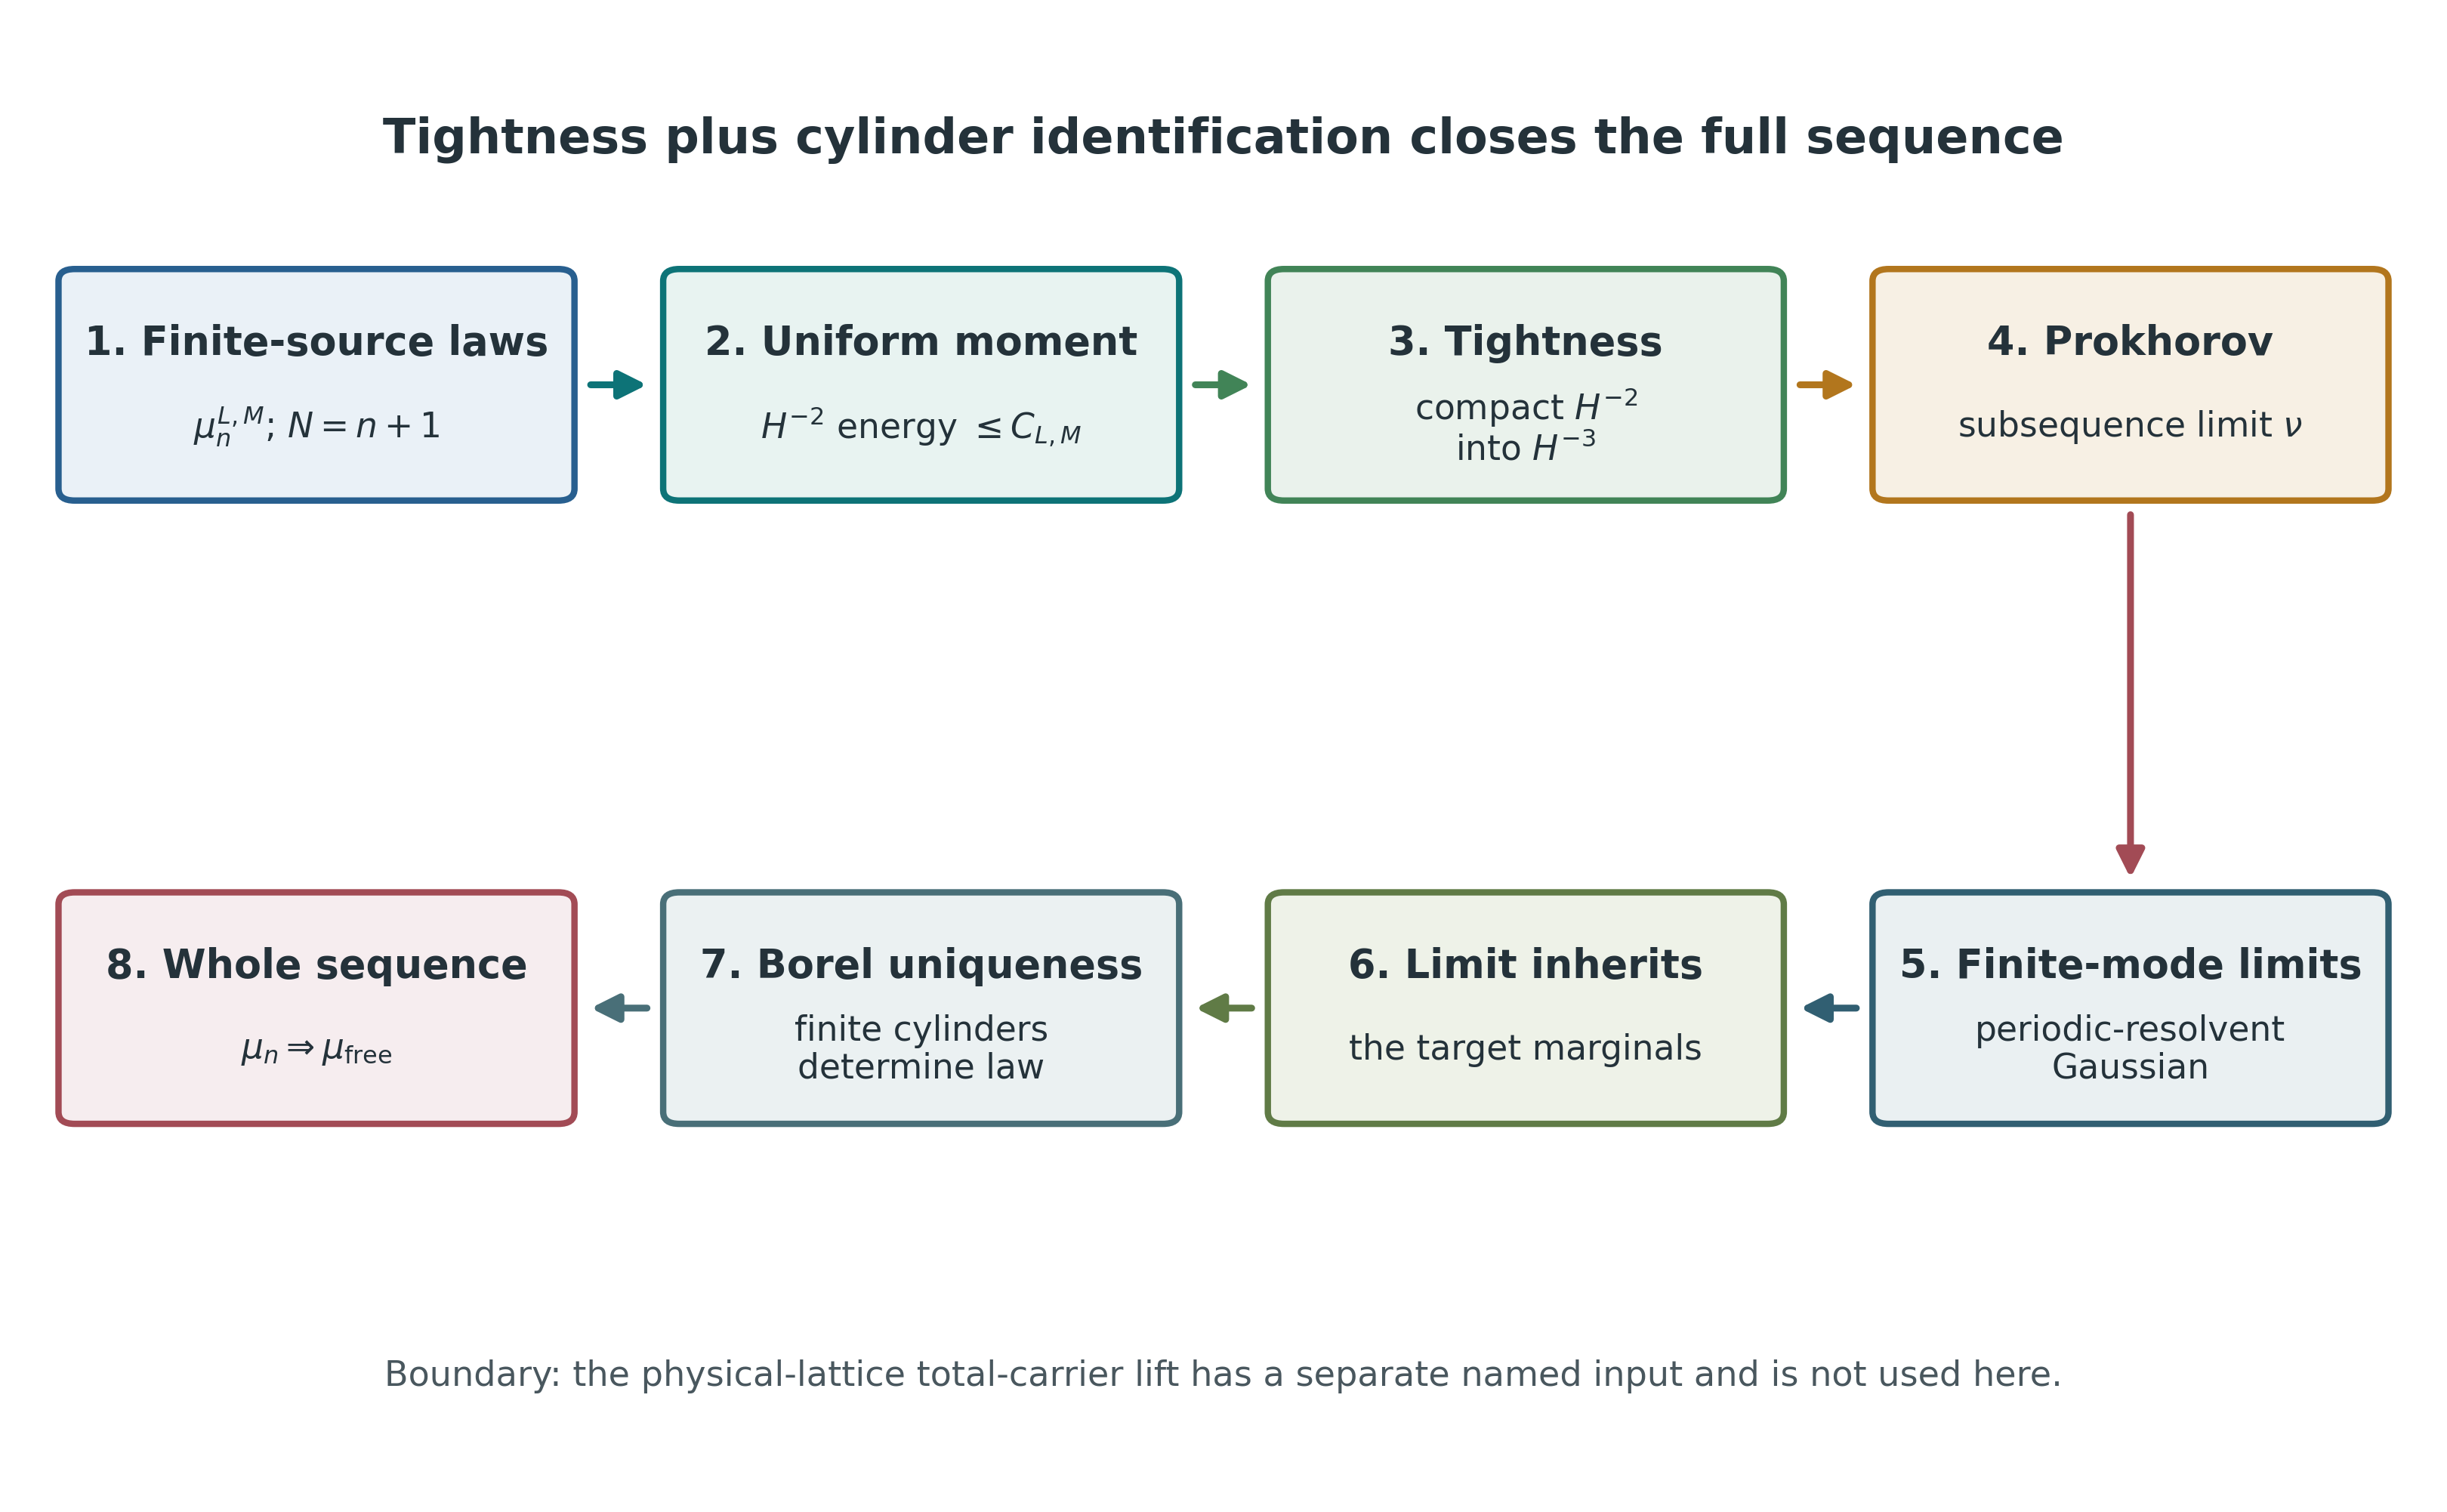
\includegraphics[width=\linewidth]{figures/weak_limit_spine.png}
\caption{The spine of the limit argument. The first box is the point of departure, the finite-source lattice laws; the seven after it carry the argument: the uniform $H^{-2}$ moment; tightness on the carrier; Prokhorov extraction of a subsequential limit; the finite-mode limits from the marginal computations; the limit inherits the target marginals; cylinder-to-Borel uniqueness identifies that limit; and whole-sequence convergence closes it. The last step is the whole-sequence conclusion, not merely a subsequential one. Two inputs are not drawn, because they are settled before this half begins: the carrier construction (move~2 of \cref{sec:intro}) and the covariance limit (part of move~1), which is where the target covariance comes from. Two reading notes. The figure's own footer annotation calls the total-carrier lift a separate input that is not used here; that annotation records the development's implementation choice and is superseded by \cref{lem:lift-representative} and \cref{rem:lift-development}, which prove the paper's lift total and Borel outright. And the figure labels the mass $M$ where the text writes $m$; the index $n$ is the text's own mesh index, not the text's $N$.}
\label{fig:spine}
\end{figure}


The figure shows the spine of the argument, from the lattice laws through the
moment bound and tightness to the whole-sequence conclusion, in the order in
which the steps are proved.

What makes the argument checkable rather than merely correct is the following.

\begin{itemize}
\item The covariance limit (\cref{thm:covariance-limit}) is proved against the
  resolvent of \cref{lem:resolvent}, which is built from an energy identity and
  a Riesz adjoint and is therefore available before any Fourier series is
  written.  The symbol is an output of that construction, not a postulate that
  the lattice limit is then matched to.  The limit of the sampled covariance is
  therefore settled independently of what the series says it is.
\item The carrier is the explicit weighted $\ell^2$ space of
  \cref{def:carrier-hminus3}.  Separability (\cref{thm:separable}) and the
  equality of cylinder and Borel sigma-algebras (\cref{thm:cylinder-borel}) are
  proved for that space, so the two structural facts that a measure-theoretic
  limit normally assumes are theorems here.
\item The conclusion (\cref{thm:main}) is about the whole sequence, and
  \cref{cor:uniqueness} shows that no subsequence can produce a different limit.
  The two quantitative inputs are the uniform moment (\cref{thm:uniform-moment})
  and the marginal limits (\cref{thm:finite-family}); the identification step
  rests on \cref{thm:cylinder-uniqueness}.
\item The target law of each finite family is computed and not selected.  Its
  characteristic function is derived from the resolvent pairing of step~1
  (\cref{thm:char-function}) and its covariance entries are matched to that
  pairing, so the marginal limits are a consequence of the covariance limit
  rather than a second, independent assumption about what the limit should be.
\end{itemize}

Two items are stated in the underlying documents without a paper-level
derivation, and are derived in full here: the uniform trace constant behind the
moment bound (\cref{lem:trace-constant}) and the entrywise identification of the
paired cosine/sine covariance matrix (\cref{lem:hC-identification}).  Both are
elementary once the normalisation of the lattice covariance is fixed, and both
are needed before the tightness and marginal steps can be completed.

The scope of the result is deliberately narrow.  What converges is the
finite-source Fourier pushforward $\mu_N$ of the lattice Gaussian law, which
\cref{lem:lift-representative} identifies as the law of a Borel carrier-valued
map of the lattice field, so ``the lattice field laws converge'' is asserted in
exactly that sense and no other: the statement is about the law of the Fourier
coefficient sequence, not about a particular total lift of the development
(\cref{rem:lift-development}).  No rate of convergence,
no exponential tail and no quantitative modulus is claimed: the tightness
argument is Markov's inequality applied to a second moment of the norm, and nothing else.  No
interacting ultraviolet limit and no Osterwalder--Schrader reconstruction is
proved; the theory constructed here is the free one.  The carrier, its weights
and every object in the measure limit are two-dimensional, and no dimensional
generalisation of them is claimed.  \Cref{sec:scope} states the boundary in full
and \cref{sec:lean-boundary} states which layer of the argument is
machine-checked.

% ==========================================================================
%  Section 2 -- Setting.  Owner: W02.  Frozen label: sec:setting.
%
%  This file fixes, and proves nothing: the torus and its test space
%  (def:torus), the pairing normalisation (rem:v-normalisation), the index
%  sets and the three weights (def:modes), the norm the weights are built
%  from (def:weight-supnorm), the negative-Sobolev carriers (def:carrier-hs),
%  the fixed-volume regime and the N/n dictionary (hyp:volume), the lattice
%  configuration space and the two symbols (eq:lattice-symbol,
%  eq:continuum-symbol), the two borrowed facts (ext:fourier-basis,
%  ext:summability), the dimensional caveat (rem:dimension) and the four
%  conventions a reader can get wrong (rem:conventions).
% ==========================================================================
\section{Setting}\label{sec:setting}

This section fixes the objects and the conventions that the rest of the paper
uses, and it proves nothing substantive. \Cref{def:torus} fixes the torus, its
test space and the Fourier coefficient; \cref{rem:v-normalisation} the
normalisation of the pairings; \cref{def:modes,def:weight-supnorm} the index
sets and the three weights; \cref{def:carrier-hs} the negative-Sobolev sequence
spaces that carry the measures and the energy. \Cref{hyp:volume} fixes the
fixed-volume regime and the dictionary between the two ways of indexing it. Two
background facts are stated: one is borrowed, as an external
theorem (\cref{ext:fourier-basis}), and the other is proved outright below
(\cref{ext:summability}). No probabilistic object is
introduced here: the lattice laws belong to \cref{sec:lattice}.

\subsection{The torus, its test space, and the Fourier coefficient}

\begin{definition}[The periodic torus and its test space]\label{def:torus}
Let $L>0$. The \emph{periodic torus} is $\Torus:=\R^2/(L\Z)^2$, identified
throughout with the half-open cell $[0,L)^2$; its volume is $V:=L^2$. A
\emph{test function} is a bounded continuous $f:\R^2\to\R$ that is
$L$-periodic in each coordinate,
\[
  f(x+Le_i)=f(x)\qquad\text{for } i=1,2 \text{ and all } x\in\R^2 ,
\]
where $e_1,e_2$ are the standard unit vectors, so a test function is a bounded
continuous real function on $\Torus$. The
trigonometric polynomials are uniformly dense in the set of test functions ---
a standard fact, recorded here for orientation; no step below spends it, because
every approximation in this paper is a finite-mode truncation of a series whose
terms are already explicit. The \emph{Fourier coefficient} of
a test function $f$ at the mode $k\in\Z^2$ is
\begin{equation}\label{eq:fourier-coefficient}
  F(k):=\int_{[0,L]^2} f(x)\,e^{-2\pi i\,k\cdot x/L}\,\dd x ,
\end{equation}
the integral being taken over the physical cell of Lebesgue measure $V$, so that
$F(k)$ carries the dimension of $f$ times volume. There is deliberately no
factor $V^{-1}$ in \eqref{eq:fourier-coefficient}.
\end{definition}

\begin{remark}[The pairings carry $V^{-1}$]\label{rem:v-normalisation}
The coefficient \eqref{eq:fourier-coefficient} is the \emph{integral-normalised}
one. Every Fourier pairing written later has the shape
$V^{-1}\sum_k\overline{F(k)}\,G(k)\,\rho(k)$ with a symbol $\rho$: the factor
$V^{-1}$ belongs to the pairing, never to the coefficient. The competing
convention is the orthonormal one attached to the basis of
\cref{ext:fourier-basis}, whose coefficient at $k$ is $V^{-1}F(k)$; the change of
variables between the two is \cref{lem:haar-lebesgue}. Both conventions occur
below, and interchanging them loses exactly one factor of $V=L^2$.
\end{remark}

\subsection{Modes, weights, and which norm enters them}

\begin{definition}[Fourier index set and weights]\label{def:modes}
The \emph{continuum index set} is $\Z^2$; the \emph{lattice index set} is
$I_N:=(\Z/N\Z)^2$, with $N\in\N$ as in \cref{hyp:volume}. For $k\in\Z^2$ put
$\norm{k}_\infty:=\max\{\abs{k_1},\abs{k_2}\}$. The weights of this paper are
functions of this sup norm and of nothing else; the Euclidean norm enters only
the symbols \eqref{eq:lattice-symbol}--\eqref{eq:continuum-symbol}. The weights
are
\begin{equation}\label{eq:weights}
  w_3(k)=
  \begin{cases}
    1, & k=0,\\[2pt]
    \norm{k}_\infty^{-6}, & k\neq0,
  \end{cases}
  \qquad
  w_2(k)=
  \begin{cases}
    0, & k=0,\\[2pt]
    \norm{k}_\infty^{-4}, & k\neq0,
  \end{cases}
\end{equation}
together with the \emph{full} weight $\widetilde w_2$, which agrees with $w_2$
at every $k\neq0$ and takes the value $\widetilde w_2(0)=1$. Thus $w_3$ and
$\widetilde w_2$ are positive at every mode, the origin included, whereas $w_2$
is not.
\end{definition}

The three weights are not interchangeable, and everything below depends on
keeping them apart. The seminorm weight $w_2$ annihilates the zero mode and
enters only where that mode is restored by a separate additive term --- the split
that makes the weighted trace finite
(\cref{thm:uniform-moment,lem:trace-constant}). The full
weight $\widetilde w_2$ is positive everywhere, so the weighted sum it defines
is an honest norm and its sublevel sets are the compact sets of the argument
(\cref{thm:compact-tail}). The weight $w_3$ is positive everywhere for the same
reason as $\widetilde w_2$, and its weighted space carries the measures
(\cref{def:carrier-hs}).

\begin{definition}[The sup norm on the mode lattice]\label{def:weight-supnorm}
For $k\in\Z^2$ the symbol $\norm{k}_\infty$ denotes the sup norm
$\max_i\abs{k_i}$ of \eqref{eq:weights}, and $\abs{k}$ the Euclidean norm
$(\sum_ik_i^2)^{1/2}$. Every weight of this paper is a function of
$\norm{k}_\infty$ alone, every symbol of
\cref{eq:lattice-symbol,eq:continuum-symbol} a function of $\abs{k}$. The two
are equivalent, $\norm{k}_\infty\le\abs{k}\le 2^{1/2}\norm{k}_\infty$ in two
dimensions, and they give the same summability threshold
(\cref{ext:summability}); they are not interchangeable inside an estimate,
because for $k$ with $\abs{k_1}\neq\abs{k_2}$ the two differ and
$\norm{k}_\infty^{-4}\neq\abs{k}^{-4}$.
\end{definition}

\subsection{Negative-Sobolev carriers}

\begin{definition}[Negative-Sobolev sequence spaces]\label{def:carrier-hs}
Let $\mathcal W=(\mathcal W(k))_{k\in\Z^2}$ be a weight with $\mathcal W(k)>0$
for every $k$, and put
\begin{equation}\label{eq:ell2s}
  \ell^2(\Z^2;\mathcal W):=
  \Bigl\{c=(c_k)_{k\in\Z^2}\in\C^{\Z^2}:
  \sum_{k\in\Z^2}\mathcal W(k)\abs{c_k}^2<\infty\Bigr\},
\end{equation}
a Hilbert space for the inner product
$\ip{c}{d}_{\mathcal W}=\sum_k\mathcal W(k)\overline{c_k}d_k$. For $s>0$ let
\begin{equation}\label{eq:full-weight-family}
  \widetilde w_s(k)=
  \begin{cases}
    1, & k=0,\\[2pt]
    \norm{k}_\infty^{-2s}, & k\neq0,
  \end{cases}
  \qquad\text{and set}\qquad
  \HL{s}:=\ell^2(\Z^2;\widetilde w_s).
\end{equation}
The two exponents of \eqref{eq:weights} are the cases $\widetilde w_2$ and
$\widetilde w_3=w_3$ of this family. This is a definition and not a theorem: no
separately defined distribution space is identified here, in keeping with
\cref{sec:scope}. The letter $s$ is the Sobolev order, so the weight of
$\HL{s}$ decays like $\norm{k}_\infty^{-2s}$; where the \emph{decay exponent}
itself is meant below, it is written out rather than denoted by $s$, because the
two differ by a factor of two and the summability threshold is stated in the
decay exponent.
\end{definition}

Two of these spaces occur, with two different jobs, and neither exponent may be
relabelled. The \emph{carrier} is $\HL{3}$: the lattice laws of
\cref{sec:lattice} are Borel probability measures on its completion, and the weak
convergence asserted in \cref{sec:main} is weak convergence there. The
\emph{energy} is $\HL{2}$: the uniform moment of \cref{thm:uniform-moment} is an
$\HL{2}$ quantity. The inclusion $\HL{2}\subseteq\HL{3}$ is
\cref{prop:completion}, and it is the ratio $w_3/\widetilde w_2=\norm{k}_\infty^{-2}$
that tends to zero --- the $\HL{3}$ weight decays \emph{faster}, not the $\HL{2}$ one ---
which is what makes an $\HL{2}$-sublevel set have small $\HL{3}$-tails, hence
relatively compact closure (\cref{thm:compact-tail}).

A point of $\HL{3}$ may be written as its family of Fourier coefficients, with
the weighted norm \eqref{eq:full-weight-family}, or as the family of
\emph{stored coordinates} obtained by applying $\sqrt{\widetilde w_3(k)}$ to
each coefficient; the two differ by the diagonal isometry of
\cref{def:carrier-hminus3}, and \cref{rem:two-families} says which one each
formula below is written in. The deweighting is defined on all of $\HL{3}$
precisely because $\widetilde w_3(k)>0$ at every $k$, the zero mode included
(\cref{eq:weights}) --- which is why the zero mode of the $\HL{3}$ weight is $1$
and not $0$. Computing an $\HL{2}$ norm in coordinates that already carry the
$\HL{3}$ weight multiplies it by a mode-dependent factor, which is the trap
\cref{rem:conventions} warns about.

\subsection{Fixed volume, the two symbols, and a borrowed fact}

\begin{hypothesis}[Fixed physical volume]\label{hyp:volume}
Throughout, $L>0$ and the mass $m>0$ are fixed. The lattice spacing $a>0$ and
the lattice size $N\in\N$ satisfy
\begin{equation}\label{eq:fixed-volume}
  aN=L,
\end{equation}
and the sequence of lattices is indexed by $n\in\N$ through
\begin{equation}\label{eq:index-dictionary}
  N=n+1,\qquad a=a_n=\frac{L}{n+1}\ .
\end{equation}
\end{hypothesis}

\Cref{hyp:volume} also fixes the bookkeeping that the two halves of the paper
index differently. The mathematics below writes $N$ for the lattice size and
passes to $N\to\infty$; the machine development of \cref{sec:lean-overview}
indexes its statements by $n$ and derives $N=n+1$, $a=L/(n+1)$.
\Cref{eq:index-dictionary} is the whole dictionary, with one consequence: the
mesh is never a free parameter, so only $L$, $m$ and $n$ are free below.

Fixed volume buys one thing, and the argument rests on it: a symbol limit.
Because \eqref{eq:fixed-volume} forces $a=L/N\to0$ at fixed $L$, the lattice
symbol below approaches the continuum symbol mode by mode at each fixed $k$, and
it is exactly because the spacing vanishes while $L$ is held fixed that the limit
is not a rescaling of the field. Fixed volume buys no modulus: no rate, no
exponential tail and no quantitative convergence statement is proved here
(\cref{sec:scope}), and the limit is not asserted to be an $L^2$ function.

Two symbols are used from here on, and neither identity is proved here: the
first is the symbol of the operator of
\cref{def:lattice-laplacian,prop:operator}, the second that of the resolvent of
\cref{lem:resolvent}. The lattice configuration space is
$\R^{I_N}$: a configuration assigns a real number to each site $x\in I_N$, and
the site $x$ has the physical representative $ax\in[0,L)^2$. The lattice symbol
and the continuum symbol are
\begin{equation}\label{eq:lattice-symbol}
  \lambda_N(p):=m^2+4a^{-2}\sum_{i=1}^{2}\sin^2\Bigl(\frac{\pi p_i}{N}\Bigr),
  \qquad p\in I_N ,
\end{equation}
\begin{equation}\label{eq:continuum-symbol}
  \lambda(k):=m^2+\Bigl(\frac{2\pi}{L}\Bigr)^{2}\abs{k}^2 ,
  \qquad k\in\Z^2 .
\end{equation}
The expression \eqref{eq:lattice-symbol} is well defined on the residue class
$p_i\in\Z/N\Z$ because $\sin^2(\pi t)$ is $1$-periodic in $t$. Both symbols are
real and at least $m^2>0$, so no denominator formed from them vanishes.

\begin{external}[Torus Fourier basis]\label{ext:fourier-basis}
Let $z=x/L\in[0,1)^2$ and let $\dd z$ be Lebesgue measure on the unit cell, whose
total mass is $1$. The family $z\mapsto e^{2\pi i\,k\cdot z}$, $k\in\Z^2$, is a
complete orthonormal basis of $L^2([0,1)^2,\dd z;\C)$.
\end{external}

\Cref{ext:fourier-basis} is used as a black box, and no other completeness
statement is needed below. It is quoted in this orthonormal form because that is
the form in which tests are paired with the resolvent in \cref{sec:covariance};
the factor that reconciles it with \eqref{eq:fourier-coefficient} is the
$V^{-1}$ of \cref{rem:v-normalisation}, whose proof is \cref{lem:haar-lebesgue}.

\begin{lemma}[Summability of the weights]\label{ext:summability}
In two dimensions both of the following series converge:
\begin{equation}\label{eq:summability}
  \sum_{k\ne0}\norm{k}_\infty^{-4}<\infty,
  \qquad
  \sum_{k\ne0}\norm{k}_\infty^{-6}<\infty .
\end{equation}\end{lemma}

\begin{proof}
The two sums are explicit. The shell $\norm{k}_\infty=q$, $q\ge1$, carries
$(2q+1)^2-(2q-1)^2=8q$ modes, and on that shell $\norm{k}_\infty^{-r}=q^{-r}$, so
each sum is $8\sum_{q\ge1}q^{1-r}$ with $r=4$ respectively $r=6$; such a series
converges exactly when $r>2$. The inequality that matters is therefore $2<4$ and
$2<6$: \emph{the decay exponent of the weight must exceed the dimension}.
\end{proof}

The two values are worth naming, because the constants below carry them:
\[
  \sum_{k\ne0}\norm{k}_\infty^{-4}=8\zeta(3),
  \qquad
  \sum_{k\ne0}\norm{k}_\infty^{-6}=8\zeta(5).
\]

\begin{remark}[The exponents are the two-dimensional ones]\label{rem:dimension}
The threshold just computed is that the decay exponent exceeds $d$, and here
$d=2$. In $d=4$ the decay exponent $4$ of $\widetilde w_2$ would be critical
rather than summable, so the pair $w_2,w_3$ of \eqref{eq:weights} is a
two-dimensional pair; the paper claims nothing about dimension four and offers
no general one. The source of
\cref{sec:covariance} is registered for a general dimension $d$, but this paper
writes it in two dimensions, like everything else here: the test functions are
functions on $\R^2$, and the shell count in the last step of its proof uses
$d=2$. The measure chain therefore uses $d=2$ throughout, with no statement and
no object of this paper claimed in another dimension (\cref{sec:scope}).
\end{remark}

\begin{remark}[Four conventions a reader can get wrong]\label{rem:conventions}
Each of the following is settled above, and each is easy to reverse by accident.
\emph{(i) Integral versus orthonormal normalisation:} \eqref{eq:fourier-coefficient}
carries no $V^{-1}$, the pairing carries it, and the probability-torus form
appears only where a test is paired with the resolvent in \cref{sec:covariance}
(\cref{rem:v-normalisation,lem:haar-lebesgue}). \emph{(ii) Sup norm versus
Euclidean norm:} the weights are stated for $\norm{k}_\infty$ and the symbols
for $\abs{k}$, and the two must not be exchanged inside an estimate
(\cref{def:weight-supnorm}). \emph{(iii) Seminorm versus full weight:} $w_2$
vanishes at the zero mode and is usable only where that mode is supplied
separately, while $\widetilde w_2$ and $w_3$ are positive everywhere and are
what the norm and the compactness argument use
(\cref{def:modes,def:carrier-hs}). \emph{(iv) Carrier versus energy exponent:}
$\HL{3}$ is the carrier of the laws and the topology of weak convergence,
$\HL{2}$ the exponent of the energy and of the uniform moment, and neither may
stand in for the other
(\cref{def:carrier-hs,thm:uniform-moment,sec:tightness}).
\end{remark}

% ==========================================================================
%  Section 3 -- The lattice free field and its physical-volume law.  Owner: W03.
%  Frozen labels (CONTRACT section 4): sec:lattice, def:lattice-laplacian,
%  prop:operator, def:gj-measure, def:finite-source-lift, rem:lattice-input,
%  lem:haar-lebesgue; added here: lem:finite-parseval and the eq: labels.
%
%  Proved in this file: the eigenfunction identity and the positivity bound
%  (prop:operator), finite Parseval (lem:finite-parseval), the Haar normalisation
%  (lem:haar-lebesgue).  Defined: the Gaussian operator and its symbol, the
%  physical lattice Gaussian law, the finite-source Fourier lift and its law.
%  The lattice covariance is an input (rem:lattice-input).  Nothing here states
%  a limit; the two limits are named in the closing paragraph.
% ==========================================================================
\section{The lattice free field and its physical-volume law}\label{sec:lattice}

This section fixes the two objects that Part~I consumes. \Cref{def:lattice-laplacian} introduces the
discrete Laplacian and the Gaussian operator; \cref{prop:operator} proves the eigenfunction identity and
the positivity bound that every later estimate uses. \Cref{lem:finite-parseval} is the one estimate of the
paper that spends boundedness, \cref{def:gj-measure} is the physical lattice Gaussian law, and
\cref{def:finite-source-lift} carries that law to the weighted Fourier side. \Cref{lem:haar-lebesgue}
reconciles the two Fourier normalisations of \cref{rem:v-normalisation}. Two points made in passing matter
later: the lattice covariance is an input and not derived here (\cref{rem:lattice-input}), and the spacing
enters more than once, in different powers (\cref{def:gj-measure}).

\subsection{The discrete Laplacian and the Gaussian operator}

\begin{definition}[The discrete Laplacian and the Gaussian operator]\label{def:lattice-laplacian}
Let $N\ge1$ and $a=L/N$ as in \cref{hyp:volume}. A \emph{configuration} is a real function $\omega$ on the
lattice $I_N=(\Z/N\Z)^2$ of \cref{def:modes}; the lattice configuration space is $\R^{I_N}$, and we also
admit complex $u:I_N\to\C$. With $e_1,e_2$ the unit residues, the \emph{discrete Laplacian} is
\begin{equation}\label{eq:laplacian}
  (\Delta_au)(x):=a^{-2}\sum_{i=1}^{2}\bigl(u(x+e_i)+u(x-e_i)-2u(x)\bigr),
\end{equation}
the two oriented neighbours being subtracted and added exactly once, so that \eqref{eq:laplacian} keeps
its form even when $N\le2$. The \emph{Gaussian operator} is
\begin{equation}\label{eq:gaussian-operator}
  Q:=m^2-\Delta_a ,
\end{equation}
and we write $A_N:=Q$ when $Q$ acts on configurations against the \emph{counting} inner product, the one
attached to the vector space $\R^{I_N}$:
\begin{equation}\label{eq:counting-inner-product}
  \ip{u}{v}_{\mathrm{counting}}:=\sum_{x\in I_N}u(x)v(x),
\end{equation}
so that $A_N^{-1}$ is the inverse of $Q$. For $p\in I_N$ the \emph{character} at $p$ is the function
\[
  \chi_p(x):=\exp\bigl(2\pi i\,p\cdot x/N\bigr),\qquad x\in I_N ,
\]
the product $p\cdot x$ being read modulo $N$.
\end{definition}

\begin{proposition}[Operator facts]\label{prop:operator}
$\Delta_a$ is a symmetric real matrix, hence self-adjoint, and $Q$ is positive definite with spectrum
contained in $[m^2,\infty)$. Consequently $Q$ is invertible and has a positive square root $Q^{1/2}$, and
$\C^{I_N}$ has an orthonormal basis of eigenvectors of $Q$. The eigenfunctions are the characters, with
eigenvalues the symbol $\lambda_N$ of \eqref{eq:lattice-symbol}:
\begin{equation}\label{eq:eigen-identity}
  \Delta_a\chi_p=-4a^{-2}\Bigl(\sum_{i=1}^{2}\sin^2\frac{\pi p_i}{N}\Bigr)\chi_p ,
  \qquad
  Q\chi_p=\lambda_N(p)\,\chi_p ,
\end{equation}
and $\lambda_N(p)\ge m^2>0$ for every $p\in I_N$.
\end{proposition}

\begin{proof}
\emph{The eigenfunction identity.} Translating the argument of a character multiplies it by a scalar: for
$i=1,2$ and every $x$,
\[
  \chi_p(x+e_i)=\zeta_i\chi_p(x),\qquad \chi_p(x-e_i)=\zeta_i^{-1}\chi_p(x),
  \qquad \zeta_i:=e^{2\pi ip_i/N},
\]
because $p_i(x_i+1)\equiv p_ix_i+p_i$ modulo $N$. Inserting this into \eqref{eq:laplacian} gives
$(\Delta_a\chi_p)(x)=a^{-2}\sum_i(\zeta_i+\zeta_i^{-1}-2)\chi_p(x)$, and Euler's formula gives
$\zeta_i+\zeta_i^{-1}-2=2\cos(2\pi p_i/N)-2=-4\sin^2(\pi p_i/N)$. Hence the eigenfunction identity of
\eqref{eq:eigen-identity}; the relation $Q\chi_p=\lambda_N(p)\chi_p$ then follows from the definition
\eqref{eq:lattice-symbol} of the symbol together with $Q=m^2-\Delta_a$.

\emph{Positivity.} Each summand $4a^{-2}\sin^2(\pi p_i/N)$ of \eqref{eq:lattice-symbol} is a nonnegative
real number, so $\lambda_N(p)\ge m^2$; and $m>0$ by \cref{hyp:volume}.

\emph{An explicit orthonormal eigenbasis.} Summing the one-coordinate geometric series and using
$\zeta^N=1$ for $\zeta=e^{2\pi i/N}$,
\[
  \sum_{x\in I_N}\chi_{-p}(x)\chi_q(x)
  =\prod_{i=1}^{2}\sum_{x_i\in\Z/N\Z}e^{2\pi i(q_i-p_i)x_i/N}=N^2\mathbf 1_{p=q} ,
\]
so the $N^2$ characters are pairwise orthogonal and nonzero, hence a basis of $\C^{I_N}$; scaled by
$N^{-1}$ they are orthonormal, and \eqref{eq:eigen-identity} makes each of them an eigenvector.

\emph{Self-adjointness and the spectrum.} The coefficient of $u(y)$ in $(\Delta_au)(x)$ is $-2a^{-2}$ when
$y=x$, $a^{-2}$ when $y-x=\pm e_i$ for one $i$, and $0$ otherwise; this is symmetric in $x$ and $y$, so
$\Delta_a$ is a symmetric real matrix, hence self-adjoint, and $Q$ is too. On the basis just exhibited $Q$
acts diagonally with the real entries $\lambda_N(p)$, so its spectrum is exactly
$\{\lambda_N(p):p\in I_N\}\subseteq[m^2,\infty)$: the operator is positive definite, hence invertible. A
positive definite symmetric matrix has a positive definite symmetric square root, and that is the
finite-dimensional spectral theorem, the only fact named in this proof; the eigenbasis itself is
exhibited above rather than postulated. Write $Q^{1/2}$ for that root.
\end{proof}

\begin{lemma}[Finite Parseval]\label{lem:finite-parseval}
Let $f,g:\R^2\to\R$ be bounded, and for $p\in I_N$ let
\begin{equation}\label{eq:sampled-coefficient}
  F_N(p):=a^2\sum_{x\in I_N}f(ax)\,\chi_{-p}(x),\qquad
  G_N(p):=a^2\sum_{x\in I_N}g(ax)\,\chi_{-p}(x)
\end{equation}
be the sampled coefficients at the physical points $ax$ of \cref{hyp:volume}, the factor $a^2$ being the
area of one cell. Then
\begin{equation}\label{eq:parseval}
  \sum_{p\in I_N}\overline{F_N(p)}\,G_N(p)=Va^2\sum_{x\in I_N}f(ax)g(ax),
  \qquad
  \sum_{p\in I_N}\abs{F_N(p)}^2=Va^2\sum_{x\in I_N}\abs{f(ax)}^2\le V^2\norm{f}_\infty^2 .
\end{equation}
\end{lemma}

\begin{proof}
Summing the one-coordinate geometric series over modes instead of over sites gives the dual orthogonality
relation $\sum_{p\in I_N}\chi_p(x)\chi_{-p}(y)=N^2$ when $x=y$ and $0$ otherwise. Since $f$ is real,
$\overline{\chi_{-p}(x)}=\chi_p(x)$; inserting \eqref{eq:sampled-coefficient} and interchanging the finite
sums therefore collapses the cross terms onto the diagonal:
\[
  \sum_{p\in I_N}\overline{F_N(p)}\,G_N(p)
  =a^4\!\!\sum_{x,y\in I_N}\!\!f(ax)g(ay)\sum_{p\in I_N}\chi_p(x)\chi_{-p}(y)
  =a^4N^2\sum_{x\in I_N}f(ax)g(ax).
\]
The bilinear identity of \eqref{eq:parseval} follows from $a^2N^2=a^2\cdot L^2/a^2=V$; the diagonal one is
the case $g=f$, and $a^2\sum_x\abs{f(ax)}^2\le a^2N^2\norm{f}_\infty^2=V\norm{f}_\infty^2$.
\end{proof}

This is the only place in Part~I where a test is spent through boundedness rather than through smoothness:
the bound is $\norm{f}_\infty$ alone, and that is what lets \cref{sec:covariance} work with bounded
continuous periodic tests and ask for no derivative.

\subsection{The physical lattice Gaussian law}

\begin{definition}[The physical lattice Gaussian law]\label{def:gj-measure}
With $A_N=Q$ of \eqref{eq:gaussian-operator}, put
\begin{equation}\label{eq:gj-covariance}
  C_N:=a^{-1}A_N^{-1/2},\qquad\text{so that}\qquad C_N^2=a^{-2}A_N^{-1};
\end{equation}
the squared object $C_N^2$ is the covariance operator. The \emph{physical lattice Gaussian law}
$\mu^{\mathrm{GJ}}_N$ is the centred Gaussian Borel probability measure on $\R^{I_N}$ that is the law of
$C_N\xi$ for a standard Gaussian vector $\xi$ on $\R^{I_N}$, so that $C_N^2$ is its covariance operator. Its
test averages are
$\omega\mapsto\omega(f):=\sum_{x\in I_N}a^2f(ax)\,\omega(x)$, so that
$\omega(f)=\ip{b}{\omega}_{\mathrm{counting}}$ with the sampled vector $b_x:=a^2f(ax)$, $x\in I_N$. For
$b,c\in\R^{I_N}$ the covariance pairing is therefore
\begin{equation}\label{eq:gj-pairing}
  \ip{C_Nb}{C_Nc}=a^{-2}\ip{b}{A_N^{-1}c}_{\mathrm{counting}} .
\end{equation}
It is the factor $C_N$, not the operator $C_N^2$, that the rest of Part~I calls the lattice covariance.
\end{definition}

Only two properties of $\mu^{\mathrm{GJ}}_N$ are used later, and they are its operative content here. The
mean is exactly zero: $\int\omega(f)\,\mu^{\mathrm{GJ}}_N(\dd\omega)=0$ for every bounded $f$, because
$\omega(f)$ is linear in $\omega$ and the law is centred. The covariance is the inverse-mass identity
\eqref{eq:gj-pairing} in sampled form: with $b_x=a^2f(ax)$ and $c_x=a^2g(ax)$,
\begin{equation}\label{eq:sampled-covariance}
  \operatorname{Cov}\bigl(\omega(f),\omega(g)\bigr)
  =\ip{C_Nb}{C_Nc}
  =a^{-2}\ip{b}{A_N^{-1}c}_{\mathrm{counting}}
  =a^2\ip{f}{A_N^{-1}g}_{\mathrm{counting}} ,
\end{equation}
the last equality because the counting sum picks up one factor $a^2$ per sampled vector. No other
property of $\mu^{\mathrm{GJ}}_N$ enters any estimate below.

Where the powers of $a$ sit is worth stating once, explicitly, because the factors pull in opposite
directions and a reader who cancels them gets a constant wrong. There are three occurrences and they have
three different jobs. \emph{(i)} The cell area $a^2$ sits on the \emph{test evaluation}: it is the
quadrature weight of the sum $\omega(f)=\sum_xa^2f(ax)\omega(x)$, hence part of the sampled vector
$b_x=a^2f(ax)$ in \eqref{eq:sampled-covariance}. \emph{(ii)} The covariance factor carries
$(a^2)^{-1/2}=a^{-1}$, and the pairing \eqref{eq:gj-pairing} squares it, so $a^{-2}$ sits on the bilinear
form. \emph{(iii)} The
same $a^2$ reappears inside the per-site vector of the lift \eqref{eq:lift}, where it is again the cell
area and is again a quadrature weight, this time a Fourier one. The cancellation between \emph{(i)} and
\emph{(ii)} is exact and leaves the single factor $a^2$ of \eqref{eq:sampled-covariance}, since
$a^{-2}(a^2)^2=a^2$. The $a^2$ of \emph{(iii)} is not the inverse of the $a^{-2}$ of \emph{(ii)}: the two
belong to different functionals, and neither may be cancelled against the other.

\begin{remark}[The lattice covariance is an input]\label{rem:lattice-input}
$C_N$ is data: \eqref{eq:gj-covariance} fixes it, and \cref{prop:operator} is what makes that
specification consistent, since $Q$ is then invertible with a positive square root. It is not derived here
from any field-theoretic construction, and no property of $C_N$ beyond exact zero mean and
\eqref{eq:gj-pairing} is used anywhere below. The name GJ attached to this normalisation records which
power of the spacing is meant --- namely $a^{-1}$ per factor in \eqref{eq:gj-covariance} --- and it is a
name and not a citation: no step of the proof is taken from a reference.
\end{remark}

\subsection{The finite-source Fourier lift and its induced law}

\begin{definition}[The finite-source Fourier lift]\label{def:finite-source-lift}
For a configuration $\omega\in\R^{I_N}$ and a mode $p\in\Z^2$ put
\begin{equation}\label{eq:lift}
  (L_N\omega)(p):=\sqrt{w_3(p)}\;a^2\sum_{x\in I_N}\omega(x)\,e^{-2\pi i\,p\cdot(ax)/L},
\end{equation}
with $w_3$ the weight of \cref{def:modes}, and let
\begin{equation}\label{eq:finite-source-law}
  \mu_N:=(L_N)_*\,\mu^{\mathrm{GJ}}_N
\end{equation}
be the image of the law of \cref{def:gj-measure} under $L_N$.
\end{definition}

The phase in \eqref{eq:lift} is the physical one, $e^{-2\pi i\,p\cdot(ax)/L}$, and since $a/L=1/N$ it
equals $\chi_{-p}(x)$: the lift is the discrete Fourier transform of the sampled field, not of the residue
index, and that is what makes $a^2$ the cell area rather than a bookkeeping symbol. Because the phase has
period $N$ in each component of $p$, the family \eqref{eq:lift} is the $N^2$-periodic repetition over
$\Z^2$ of its values on $I_N$. Each entry is a finite real-linear combination of the coordinate
evaluations $\omega\mapsto\omega(x)$, so $L_N$ is Borel as a map into $\C^{\Z^2}$; and $L_N$ lands in the
carrier of \cref{def:carrier-hs}, not merely in some larger space, because with
$\norm{\omega}_1:=\sum_x\abs{\omega(x)}$,
\[
  \sum_{p\in\Z^2}\abs{(L_N\omega)(p)}^2
  \le a^4\norm{\omega}_1^2\sum_{p\in\Z^2}w_3(p)
  =a^4\norm{\omega}_1^2\Bigl(1+\sum_{p\neq0}\norm{p}_\infty^{-6}\Bigr)<\infty
\]
by \cref{ext:summability}, and $w_3\le1$ makes every weighted sum of \cref{def:carrier-hs} no larger than
this one. So \eqref{eq:finite-source-law} is the genuine pushforward of a Borel probability measure by a
Borel map into the carrier: $\mu_N(A)=\mu^{\mathrm{GJ}}_N(L_N^{-1}A)$ for Borel $A$, and $\mu_N$ is a
Borel probability measure there for every $N$.

What \eqref{eq:finite-source-law} \emph{is} is a carrier-valued representative of the lattice measure
itself, and \cref{lem:lift-representative} records this as a lemma: $L_N$ is total on the
configuration space, Borel, and lands in the carrier. What is \emph{not} claimed anywhere is a
statement about a total lift specified independently of $L_N$ --- in particular the series-defined
total lift of the machine development, where the measurability of that chosen function is an input
of the data structure rather than a construction (\cref{rem:lift-development}). The object of the
law limit is $L_N$ and the measure $\mu_N$ of \eqref{eq:finite-source-law}.

\subsection{Haar versus physical Lebesgue normalisation}

\begin{lemma}[Haar-to-physical-Lebesgue normalisation]\label{lem:haar-lebesgue}
Let $f$ be a bounded continuous $L$-periodic test, put $f_L(z):=f(Lz)$ for $z\in[0,1)^2$, and let $\dd z$
be Lebesgue measure on the unit cell, of total mass $1$. The orthonormal coefficient of $f_L$ at
$k\in\Z^2$ is
\begin{equation}\label{eq:haar-coefficient}
  (Bf_L)(k):=\int_{[0,1)^2}f(Lz)\,e^{-2\pi i\,k\cdot z}\,\dd z=V^{-1}F(k),
\end{equation}
with $F$ the integral-normalised coefficient \eqref{eq:fourier-coefficient} of \cref{def:torus}.
\end{lemma}

\begin{proof}
Substituting $x=Lz$, so that $\dd x=L^2\dd z$ and $k\cdot z=k\cdot x/L$, three steps give the claim:
\begin{align*}
  (Bf_L)(k)
  &=\int_{(0,1]^2}f(Lz)\,e^{-2\pi i\,k\cdot z}\,\dd z ,\\
  &=\int_{[0,L]^2}f(x)\,e^{-2\pi i\,k\cdot x/L}\,L^{-2}\,\dd x ,\\
  &=V^{-1}\int_{[0,L]^2}f(x)\,e^{-2\pi i\,k\cdot x/L}\,\dd x=V^{-1}F(k) .
\end{align*}
The half-open cell may be replaced by the closed one because the two differ by a Lebesgue-null set; the
phase identity $k\cdot(Lz)=L\,(k\cdot z)$ holds for negative $k$ as written, with no conjugation; and
$L^2=V$.
\end{proof}

This is the single easiest place in the paper to lose a factor of $L^d$, which in two dimensions is the
volume $V$: a change of variables pays exactly one Jacobian, and substituting the orthonormal coefficient
where the integral-normalised one is meant, inside a pairing that already carries its own $V^{-1}$
(\cref{rem:v-normalisation}), loses that factor if it is done once and injects a spurious one if it is done
twice.

\subsection{The two limits taken later}

Two limits are taken in what follows, and they are of different kinds. One is the covariance limit of
\cref{sec:covariance}: the lattice covariance pairings \eqref{eq:sampled-covariance} of bounded continuous
periodic tests are shown to converge as $N\to\infty$ at fixed $L$ and $m$, against an independently
constructed resolvent. The other is the law limit of \cref{sec:tightness}--\cref{sec:main}: the object is
the sequence $(\mu_N)$ of pushforwards \eqref{eq:finite-source-law}, each a Borel probability measure on
the carrier, and the question is what a limit of that sequence on that carrier is. Which topology carries
it, and what a limit there means, is fixed in \cref{sec:carrier}; the definitions above are what that
section and the ones after it take as given.

% ==========================================================================
%  Section 4 -- The physical-volume covariance limit.  Owner: W04.
%  Frozen label: sec:covariance.  Target 1200 words.
%
%  Contents: the two pairings (eq:pairings); the periodic massive resolvent
%  built from an energy form and a Riesz adjoint (lem:resolvent); the
%  physical-cell Riemann-sum theorem (ext:boxintegral); the lattice
%  covariance as a counting pairing with the inverse of the Gaussian operator
%  (lem:resolvent-pairing); the fixed-volume limit in five labelled steps
%  (thm:covariance-limit); and the absence of a Bessel kernel (rem:no-bessel).
%
%  Naming: the pairings are written Qcal_N, Qcal, because the letter Q is the
%  Gaussian operator m^2 - Delta_a of def:lattice-laplacian (section 3).
% ==========================================================================
\section{The physical-volume covariance limit}\label{sec:covariance}

This section proves the one analytic limit of Part~I that is not measure theory:
the covariance integrals of the physical lattice laws converge, and their limit
is a pairing with a resolvent constructed before any Fourier series is written.
\Cref{lem:resolvent} builds that resolvent from an energy form and a Riesz
representation \cite{yosida1980}, \cref{lem:resolvent-pairing} rewrites the
lattice covariance of
\cref{def:gj-measure} as a counting pairing with the inverse of the Gaussian
operator $A_N=m^2-\Delta_a$, and \cref{thm:covariance-limit} combines the two.
The objects are the pairings
\begin{equation}\label{eq:pairings}
  \mathcal Q_N(f,g):=\frac1V\sum_{p\in I_N}
    \frac{\overline{F_N(p)}\,G_N(p)}{\lambda_N(p)},
  \qquad
  \mathcal Q(f,g):=\frac1V\sum_{k\in\Z^2}
    \frac{\overline{F(k)}\,G(k)}{\lambda(k)},
\end{equation}
where $F$ is \eqref{eq:fourier-coefficient}, $F_N$ the sampled coefficient
\eqref{eq:sampled-coefficient}, and $\lambda_N,\lambda$ the symbols
\eqref{eq:lattice-symbol}--\eqref{eq:continuum-symbol}. The calligraphic letter
keeps $Q$ for the Gaussian operator of \cref{def:lattice-laplacian}, and no
other letter is free. Since
$\overline{F_N(p)}=F_N(-p)$ and both symbols are even, the sums are real for
real $f,g$; the computation is dimension-blind except in one shell count,
flagged in Step~5 below, and we write the two-dimensional case that
\cref{sec:setting} fixes.

\begin{lemma}[The periodic massive resolvent]\label{lem:resolvent}
Let $\nu$ be Lebesgue measure on $[0,1)^2$, of total mass $1$, and
$E:=L^2([0,1)^2,\nu;\C)$ with $\ip{u}{v}_E=\int\overline{u}\,v\,\dd\nu$,
conjugate-linear in the first argument. Write $b_k(z)=e^{2\pi i\,k\cdot z}$ for
the basis of \cref{ext:fourier-basis} and $B:E\to H$ for the induced isometry
onto $H:=\ell^2(\Z^2;\C)$. Put $\lambda(k)=m^2+\sum_i(2\pi k_i/L)^2$ and
$w(k):=\lambda(k)^{-1/2}$, and let $J$ and the gradient multipliers $D_i$ act
diagonally by $(Jh)(k)=w(k)h(k)$ and
$(D_ih)(k)=i\,(2\pi k_i/L)\,w(k)h(k)$; the value and gradient maps are
$jh:=B^{-1}Jh$ and $B^{-1}D_ih$. Then:
\begin{enumerate}
\item[(i)] the sesquilinear form
  \begin{equation}\label{eq:energy-form}
    \mathcal E(h,v):=m^2\ip{jh}{jv}_E+\sum_{i=1}^2\ip{D_ih}{D_iv}_E
  \end{equation}
  is the energy form of $H^1(\Torus)$ and satisfies
  $\mathcal E(h,v)=\ip{h}{v}_H$ for all $h,v\in H$, and the physical-volume
  inner product on the torus of period $L$ is $V\ip{\cdot}{\cdot}_E$;
\item[(ii)] $\{(jh,(D_ih)_i):h\in H\}$ is the closure in $E\times E^2$ of the
  pairs formed by finite trigonometric polynomials on $\Torus$ and their
  classical physical-coordinate derivatives; this is the periodic
  $H^1(\Torus)$ graph completion of the energy form in (i);
\item[(iii)] for $g\in E$ the vector $h_g:=J^*Bg$, $Rg:=jh_g$, is the unique
  element of $E$ satisfying
  \begin{equation}\label{eq:weak-equation}
    m^2\ip{Rg}{jv}_E+\sum_{i=1}^2\ip{D_ih_g}{D_iv}_E=\ip{g}{jv}_E
  \end{equation}
  for every $v\in H$, and $\norm{Rg}_E\le m^{-2}\norm{g}_E$;
\item[(iv)] $B(Rg)(k)=\lambda(k)^{-1}Bg(k)$, and
  $\ip{f}{Rg}_E=\sum_k\overline{Bf(k)}\,Bg(k)/\lambda(k)$, the series being
  absolutely convergent.
\end{enumerate}
The construction is carried out on the unit-mass $L^2$ of the torus. No
distribution-defined Sobolev space is invoked: the completion in (ii) is an
explicit graph closure of polynomials.
\end{lemma}

\begin{proof}
(i) The multipliers are diagonal in the basis $b_k$, and
\[
  m^2w(k)^2+\sum_i(2\pi k_i/L)^2w(k)^2=\lambda(k)w(k)^2=1
\]
gives
\eqref{eq:energy-form}. The identity concerns the mixed sesquilinear form, not
only its diagonal; physical volume enters only through $\dd x=V\dd\nu$.
(ii) $J$ is bounded and injective because $0<w(k)\le m^{-1}$, and
finite-support vectors are dense in $H$. A finite-support $h$ gives the
polynomial $\sum_ka(k)b_k$ with $a(k)=w(k)h(k)$, whose coordinate derivative is
$\sum_ki\,(2\pi k_i/L)\,a(k)b_k$; conversely every finite-support polynomial
arises this way, as $w(k)\ne0$. If value-gradient pairs are Cauchy in
$E\times E^2$, \eqref{eq:energy-form} makes the energy vectors Cauchy,
completeness of $H$ supplies their limit, and continuity of $j$ and $D_i$
identifies the graph limit; the range is closed.
(iii) Since $\norm{jv}_E\le m^{-1}\norm{v}_H$, the functional
$v\mapsto\ip{g}{jv}_E$ is bounded on $H$ and represented by $h_g=J^*Bg$, and
$\ip{h_g}{v}_H=\ip{g}{jv}_E$ with \eqref{eq:energy-form} gives
\eqref{eq:weak-equation}. Two solutions differ by $u$ with
$\mathcal E(u,v)=0$ for every $v$; testing $v=u$ gives $u=0$, and injectivity of
$j$ fixes the $E$-value. Testing \eqref{eq:weak-equation} with $v=h_g$ and
taking real parts gives
$m^2\norm{Rg}_E^2\le\Real\ip{g}{Rg}_E\le\norm{g}_E\norm{Rg}_E$, and we divide
when $\norm{Rg}_E\ne0$.
(iv) The adjoint identity on a single basis vector gives $(J^*c)(k)=w(k)c(k)$
because $w$ is real, so $B(Rg)(k)=w(k)^2Bg(k)=\lambda(k)^{-1}Bg(k)$;
Cauchy--Schwarz and $\lambda\ge m^2$ make the coefficient series absolutely
convergent.
\end{proof}

\begin{external}[Physical-cell Riemann sums converge]\label{ext:boxintegral}
Let $g:[0,L]^2\to\C$ be continuous, with sup-norm modulus of continuity
$\omega_g$, and partition $[0,L]^2$ into the $N^2$ cubes of side $a=L/N$. The
sum of the lower-corner sample times $a^2$ over all cubes differs from
$\int_{[0,L]^2}g\,\dd x$ by at most $V\omega_g(a)$, so these Riemann sums
converge; half-open cells give the same value, the shared boundaries being
Lebesgue null. This is the Henstock--Kurzweil box-integral theory of the
standard library, quoted and not re-proved.
\end{external}

\begin{lemma}[Lattice covariance versus resolvent pairing]\label{lem:resolvent-pairing}
Let $b,c\in\R^{I_N}$ and let $f,g$ be real $L$-periodic. Then
\begin{equation}\label{eq:counting-pairing}
  \ip{C_Nb}{C_Nc}=a^{-2}\ip{b}{A_N^{-1}c}_{\mathrm{counting}},
  \qquad
  a^2\ip{f}{A_N^{-1}g}_{\mathrm{counting}}=\mathcal Q_N(f,g).
\end{equation}
\end{lemma}

\begin{proof}
The first identity is \eqref{eq:gj-pairing} of \cref{def:gj-measure}, the
inverse-mass form in which the lattice covariance is used: $C_N$ is an input
object (\cref{rem:lattice-input}), and the power $a^{-2}$ sits in the pairing,
not in a rescaling of the field. For the second identity, use the
character eigenbasis of \cref{prop:operator}: a real lattice function $u$ has
$u(x)=V^{-1}\sum_pF_N(p)\chi_p(x)$ because $N^2a^2=L^2=V$, and
$Q\chi_p=\lambda_N(p)\chi_p$ is \eqref{eq:eigen-identity}, with $A_N=Q$ acting
in the counting inner product. Substituting both expansions into the
bilinear counting pairing and using the orthogonality
$\sum_{x\in I_N}\chi_p(x)\chi_q(x)=N^2\mathbf 1_{p+q\equiv0}$ together with
$G_N(-p)=\overline{G_N(p)}$ for real $g$ gives
\[
  a^2\ip{f}{A_N^{-1}g}_{\mathrm{counting}}
  =a^2V^{-2}N^2\sum_pF_N(p)\,\overline{G_N(p)}\,\lambda_N(p)^{-1}
  =\overline{\mathcal Q_N(f,g)}=\mathcal Q_N(f,g),
\]
the last equality because $\mathcal Q_N$ is real for real $f,g$. The powers of
$a$ are not cancelled by hand: each sampled vector carries $a^2$ against the
$a^{-2}$ of the pairing, and $N^2a^2=V$ turns the counting sum into the
normalised pairing. Together with \eqref{eq:sampled-covariance}, this writes the
covariance pairing in the symbol form the limit needs.
\end{proof}

The measure below is the physical lattice law $\mu^{\mathrm{GJ}}_N$ of
\cref{def:gj-measure}, not the finite-source pushforward $\mu_N$ whose laws
converge in \cref{sec:tightness}--\cref{sec:main}: what is proved here is a
statement about pairings, and it enters \cref{sec:marginals} as the pairwise
covariance input, since every finite cylinder coordinate of the lift is a finite
linear combination of lattice source coordinates (\cref{def:finite-source-lift});
the entrywise identification is separate (\cref{lem:hC-identification}).

\begin{theorem}[Fixed-volume covariance limit]\label{thm:covariance-limit}
Let $L>0$ and $m>0$, and let $f,g:\R^2\to\R$ be bounded continuous and
$L$-periodic. Let $a=L/N$, let $\mu^{\mathrm{GJ}}_N$ be the physical lattice law
of \cref{def:gj-measure}, write $f_L\in E$ for $z\mapsto f(Lz)$ as in
\cref{lem:haar-lebesgue}, and let $b,c\in\R^{I_N}$ be the sampled vectors
$b_x=a^2f(ax)$, $c_x=a^2g(ax)$. Then, as $N\to\infty$ with $L$ and $m$ fixed,
\begin{equation}\label{eq:three-limits}
  \begin{aligned}
    \ip{C_Nb}{C_Nc}&\longrightarrow\Real V\ip{f_L}{Rg_L}_E,\\
    \int\omega(f)\,\omega(g)\,\mu^{\mathrm{GJ}}_N(\dd\omega)
      &\longrightarrow\Real V\ip{f_L}{Rg_L}_E,\\
    \int\bigl(\omega(f)-\E\omega(f)\bigr)
         \bigl(\omega(g)-\E\omega(g)\bigr)\,\mu^{\mathrm{GJ}}_N(\dd\omega)
      &\longrightarrow\Real V\ip{f_L}{Rg_L}_E,
  \end{aligned}
\end{equation}
where $\omega(f)$ is the test average of \cref{def:gj-measure} and $\E$ is the
expectation under $\mu^{\mathrm{GJ}}_N$. Both means vanish identically in $N$, so
the second and third limits coincide.
\end{theorem}

\begin{proof}
By \cref{lem:resolvent-pairing} the first line of \eqref{eq:three-limits} is
$\mathcal Q_N(f,g)$, and the other two are the mixed second moment and the
centred covariance of the same Gaussian family. It suffices to prove
$\mathcal Q_N(f,g)\to\mathcal Q(f,g)$ and to identify $\mathcal Q$ with the
resolvent pairing, in five labelled steps.

\textbf{Step 1 (fixed-mode Riemann sums).} Let $k\in\Z^2$ and let
$p_N(k)\in I_N$ be its residue class. At the sampled physical point $t=a x$ the
phase is exactly $e^{-2\pi i\,k\cdot t/L}=e^{-2\pi i\,k\cdot x/N}$, for either
representative of the residue class, and
$t\mapsto f(t)e^{-2\pi i\,k\cdot t/L}$ is uniformly continuous on the compact
cell with sup-norm modulus of continuity $\omega_k$. \Cref{ext:boxintegral}
applied to that function gives
\begin{equation}\label{eq:fixed-mode}
  \abs{F_N(p_N(k))-F(k)}\le V\omega_k(a),
  \qquad \omega_k(a)\longrightarrow0.
\end{equation}
Continuity on the compact cell is what produces $\omega_k(a)\to0$; boundedness
alone would not, since a bounded function may oscillate across every cube of
every mesh.

\textbf{Step 2 (dispersion).} The limit $\sin t/t\to1$ gives
$4(N/L)^2\sin^2(\pi k_i/N)\to(2\pi k_i/L)^2$, hence
$\lambda_N(p_N(k))\to\lambda(k)$. Both symbols are at least $m^2>0$, so their
products and quotients converge; and the residue map is injective on
$\{k:\norm{k}_\infty\le K\}$ once $N>2K$, so for fixed $K$ the sum over the
cutoff converges term by term, real parts included.

\textbf{Step 3 (uniform denominators and tails).} Choose for each residue its
centered representative in
$\{-\lfloor N/2\rfloor,\dots,\lceil N/2\rceil-1\}^2$, which represents the
even-$N$ Nyquist frequency once. The chord bound $\sin t\ge2t/\pi$ on
$[0,\pi/2]$ gives, for centered $k$,
\begin{equation}\label{eq:uniform-denominator}
  \lambda_N(k)\ge m^2+\frac{16\norm{k}_\infty^2}{L^2},
  \qquad\text{so that}\qquad
  R_K:=m^2+\frac{16K^2}{L^2}
\end{equation}
bounds $\lambda_N$ once $\norm{k}_\infty>K$. Write $\mathcal Q_{N,K}$ and
$\mathcal Q_K$ for the sums \eqref{eq:pairings} restricted to
$\norm{k}_\infty\le K$. Cauchy--Schwarz with the finite Parseval identity
(\cref{lem:finite-parseval}) --- where boundedness of $f$ enters, and the only
place where it does --- gives
\begin{equation}\label{eq:discrete-tail}
  \abs{\mathcal Q_N-\mathcal Q_{N,K}}\le\frac{1}{VR_K}
    \Bigl(\sum_p\abs{F_N(p)}^2\Bigr)^{1/2}
    \Bigl(\sum_p\abs{G_N(p)}^2\Bigr)^{1/2}
  \le\frac{V\norm{f}_\infty\norm{g}_\infty}{R_K}
\end{equation}
uniformly in $N$ and $K\ge0$; when no modes remain outside the cutoff the left
side is zero. On the continuum side $\norm{k}_\infty\ge K+1$ gives
$\lambda(k)\ge D_K:=m^2+(2\pi/L)^2(K+1)^2$, and the same Cauchy--Schwarz
estimate on the annuli between symmetric boxes gives
\begin{equation}\label{eq:continuum-tail}
  \abs{\mathcal Q-\mathcal Q_K}
  \le\frac{V\norm{f}_\infty\norm{g}_\infty}{D_K}\longrightarrow0 .
\end{equation}
Because $4\pi^2>16$ the constant $D_K$ is at least $R_K$, so
\eqref{eq:continuum-tail} yields the tail with the constant of the discrete
estimate; that inequality is what lets one cutoff serve both sides.

\textbf{Step 4 (eventual Bessel bound).} Fix the box
$S_K=\{k:\norm{k}_\infty\le K\}$. For $N>2K$ reduction modulo $N$ is injective
on $S_K$ and identifies $S_K$ with the discrete cutoff, so nonnegativity and
\cref{lem:finite-parseval} give
\begin{equation}\label{eq:bessel-eventual}
  \sum_{k\in S_K}\abs{F_N(p_N(k))}^2\le V^2\norm{f}_\infty^2
  \qquad (N>2K).
\end{equation}
The restriction $N>2K$ is not a convenience. The bound is \emph{false} as a
statement about all $N$: a small grid aliases distinct integer modes onto one
residue, so the left side counts one coefficient several times and can exceed
the right side without bound. Since every finite $S\subseteq\Z^2$ lies in some
$S_K$, the fixed-mode limits \eqref{eq:fixed-mode} in
\eqref{eq:bessel-eventual} give
$\sum_{k\in S}\abs{F(k)}^2\le V^2\norm{f}_\infty^2$ for every finite $S$, and
bounded finite sums of a nonnegative series give square summability of
$k\mapsto F(k)$. No continuous Bessel theorem and no Fourier completeness is
assumed: this is the Bessel \emph{inequality}, and it is finite-dimensional.

\textbf{Step 5 (closed form, summability, envelope, assembly).} By (iii)--(iv)
of \cref{lem:resolvent} and the Haar-to-Lebesgue normalisation
$Bf_L(k)=V^{-1}F(k)$ of \cref{lem:haar-lebesgue},
\begin{equation}\label{eq:closed-form}
  V\ip{f_L}{Rg_L}_E
  =V\sum_k\overline{V^{-1}F(k)}\;\frac{V^{-1}G(k)}{\lambda(k)}
  =V^{-1}\sum_k\frac{\overline{F(k)}\,G(k)}{\lambda(k)}
  =\mathcal Q(f,g).
\end{equation}
So the Fourier Green pairing already carries the physical factor $L^{-2}$, and
the identification of $\mathcal Q$ with the resolvent pairing is a computation,
not a definition of $\mathcal Q$ as an operator. Absolute summability follows
from Young's inequality and $\lambda\ge m^2$,
\begin{equation}\label{eq:young}
  \abs{\frac{\overline{F(k)}\,G(k)}{\lambda(k)}}
  \le\frac{\abs{F(k)}^2+\abs{G(k)}^2}{m^2},
\end{equation}
so the series in \eqref{eq:pairings} converges, and exhaustion by symmetric
boxes gives $\mathcal Q_K\to\mathcal Q$.

A modewise majorant independent of $N$ needs more than continuity. Fix $r=d+1$,
which is $r=3$ for the case $d=2$ treated here, and
$D_r(f):=\max_i\norm{\partial_i^r f}_\infty$. The $r$-fold forward difference at
spacing $a$ is bounded by $a^rD_r(f)$ and multiplies the sampled sum by
$(\chi-1)^r$; on a nonzero centered frequency with $\norm{k}_\infty=q$ the chord
bound gives $\abs{e^{2\pi i k_i/N}-1}\ge4q/N$, and
$1/\lambda_N,1/\lambda\le L^2/(16q^2)$ yields the common envelope
\begin{equation}\label{eq:envelope}
  \abs{F_N(k)}\le V\Bigl(\frac L4\Bigr)^{r}D_r(f)\,q^{-r},
  \qquad
  \frac1V\abs{\frac{\overline{F_N(k)}\,G_N(k)}{\lambda_N(k)}}
  \le\frac{VL^2}{16}\Bigl(\frac L4\Bigr)^{2r}D_r(f)D_r(g)\,q^{-2r-2}.
\end{equation}
The sup-norm shell $\norm{k}_\infty=q$ carries $(2q+1)^d-(2q-1)^d$ modes, at
most $2d(2q+1)^{d-1}$; in $d=2$ the count is $8q$ (\cref{ext:summability}).
Since $2r+2>d$, the shell majorant is summable, and the zero mode is bounded by
$m^{-2}$ and $V\norm{f}_\infty\norm{g}_\infty$. The envelope \eqref{eq:envelope}
is a statement about $C^{r}$ periodic tests. It is \emph{not} available for all
continuous tests, and no such statement is claimed: the limit below uses no
envelope, which is why \cref{thm:covariance-limit} concerns bounded continuous
periodic tests and is not a modewise convergence theorem.

Choose $K$ so that both tails \eqref{eq:discrete-tail} and
\eqref{eq:continuum-tail} are below $\epsilon/3$; Step~2 then bounds the
fixed-cutoff error by $\epsilon/3$ for all large $N$. The triangle inequality
gives
\begin{equation}\label{eq:epsilon-three}
  \abs{\Real\mathcal Q_N(f,g)-\Real\mathcal Q(f,g)}
  \le\abs{\Real\mathcal Q_N-\Real\mathcal Q_{N,K}}
   +\abs{\Real\mathcal Q_{N,K}-\Real\mathcal Q_K}
   +\abs{\Real\mathcal Q_K-\Real\mathcal Q}
  <\epsilon,
\end{equation}
with one $K$ serving all $N$, and with no caller supplying summability, a tail
estimate or a convergence hypothesis. Transferring \eqref{eq:epsilon-three} to
the measures uses only that $\mu^{\mathrm{GJ}}_N$ is Gaussian with covariance
$C_N$ (\cref{def:gj-measure}) and has mean zero exactly at every mesh: then the
mixed second moment and the centred covariance integral both equal
$\Real\mathcal Q_N$ and hence converge to $\Real V\ip{f_L}{Rg_L}_E$ by
\eqref{eq:closed-form}. This proves \eqref{eq:three-limits}.
\end{proof}

\begin{remark}[Why no Bessel kernel appears]\label{rem:no-bessel}
The proof of \cref{thm:covariance-limit} introduces no lattice Green function
$G_a(x-y)$, no Bessel function, no modified Bessel function $K_0$, no constant
$1/(2\pi)$ or $1/(4\pi)$, and no logarithmic divergence. Every estimate is an
estimate on symbols: $\lambda_N^{-1}$ on $I_N$ and $\lambda^{-1}$ on $\Z^2$,
compared in \eqref{eq:uniform-denominator}--\eqref{eq:continuum-tail} and
controlled by \eqref{eq:bessel-eventual} and \eqref{eq:young}. Nothing is lost
by staying in the symbol domain: what is proved is a convergence statement
about pairings of bounded continuous periodic tests with the resolvent, and such
a pairing is determined by the spectral data of the resolvent on the Fourier
basis, which is exactly $\lambda^{-1}$; a positional kernel is that same data
written in another coordinate system, and producing it in closed form is a
special-function computation the argument neither performs nor needs. A text
that wrote the two-dimensional kernel $C_m(x)=K_0(m\abs{x})/(2\pi)$ here would be
naming the $x$-space representative of the \emph{same} operator on the same torus ---
the two are equal by the classical Green-function identity, and evaluating
\eqref{eq:pairings} against that kernel reproduces $\Real Q$ --- but that
identity is neither used above nor proved above, and this paper does not prove
it; what is proved is the limit of the pairings, in the symbol domain, with the
constants of this section.
Nor is a logarithmic divergence at issue: at fixed volume
$\lambda_N(0)=\lambda(0)=m^2$, and the high-frequency behaviour is absorbed by
\eqref{eq:young} through the test coefficients rather than by a kernel.
\end{remark}

With \cref{thm:covariance-limit} the analysis of the lattice symbol is finished.
Every later step of Part~I is measure theory on the carrier of
\cref{sec:carrier}: the uniform moment and compact tail of
\cref{sec:tightness}, the finite marginals of \cref{sec:marginals}, and the
assembly in \cref{sec:main}. No further symbol estimate occurs, and none is
needed.

% ==========================================================================
%  Section 5 -- The carrier and its Borel structure.  Owner: W05.
%  Frozen labels: sec:carrier, def:carrier-hminus3, prop:completion,
%  lem:coordinate-embedding, thm:separable, thm:cylinder-borel,
%  lem:lift-representative, rem:lift-development, rem:topology.
%
%  Nothing probabilistic is proved in this file: no moment estimate, no
%  tightness, no Prokhorov argument (those are sec:tightness).  What is proved
%  is that the carrier is a complete separable metric space, that the
%  coordinate maps are continuous and separate points, and that the sigma
%  algebra they generate is the Borel sigma algebra.  The open physical-lattice
%  input is stated as a hypothesis (H) and marked as used nowhere in the chain.
% ==========================================================================
\section{The carrier and its Borel structure}\label{sec:carrier}

This section builds the space on which the lattice laws of \cref{sec:lattice}
are Borel probability measures, so that convergence below is asserted against
bounded continuous functions on a concrete space. That space is an explicit
weighted sequence space over the mode lattice, and the properties a limit
theorem normally assumes of its ambient space are proved for it here:
completeness and separability (\cref{def:carrier-hminus3,thm:separable}),
continuity and point separation of the coordinate maps
(\cref{lem:coordinate-embedding}), and the equality of the sigma algebra
generated by finitely many coordinates with the Borel sigma algebra
(\cref{thm:cylinder-borel}). \Cref{prop:completion} records the comparison of
the two weights that makes the compactness argument of \cref{sec:tightness}
possible.

No moment is estimated and no tightness is proved here; that is
\cref{sec:tightness}. Nor is \cref{lem:lift-representative} proved here: it is
stated below and proved from facts of \cref{sec:lattice} and of this section.

\subsection{The carrier}

\begin{definition}[The carrier]\label{def:carrier-hminus3}
The \emph{carrier} is the weighted sequence space
\begin{equation}\label{eq:carrier}
  \mathcal C:=\HL{3}
  =\Bigl\{c=(c_k)_{k\in\Z^2}\in\C^{\Z^2}:
  \sum_{k\in\Z^2}w_3(k)\abs{c_k}^2<\infty\Bigr\},
  \qquad
  \norm{c}_{\mathcal C}^2:=\sum_{k\in\Z^2}w_3(k)\abs{c_k}^2 ,
\end{equation}
with $w_3$ the weight \eqref{eq:weights} of \cref{def:modes}, that is
$w_3(0)=1$ and $w_3(k)=\norm{k}_\infty^{-6}$ for $k\neq0$. The space $\HL{3}$
of \cref{def:carrier-hs} is spelled $\mathcal C$ from here on; it is the space
the measures below live on, and $\norm{\cdot}_{\mathcal C}$ is the norm in which
they are tight. Writing $\widehat c:=(\sqrt{w_3(k)}\,c_k)_{k\in\Z^2}$ for the
\emph{weighted family} of $c$, the map
$\Theta:\mathcal C\to\ell^2(\Z^2)$, $\Theta c=\widehat c$, is a linear isometry
of $\mathcal C$ onto the unweighted space of complex square-summable families on
the mode lattice: the carrier is $\ell^2$ of the mode lattice in weighted
coordinates. The weighted family is what the carrier stores --- the completion
of \cref{def:carrier-hs} is realised as an $\ell^2$ space whose coordinate at
$k$ is $\sqrt{w_3(k)}\,c_k$ --- so below the \emph{coordinates} of a carrier
point are the entries of $\widehat c$, while $c$ is the family of Fourier
coefficients. Its index set is $\Z^2$ throughout: the carrier, its weight and
(\cref{rem:dimension}) the measure chain are two-dimensional, and no
general-dimensional carrier is defined here.
\end{definition}

\begin{remark}[Which family a formula is written in]\label{rem:two-families}
Two families denote the same carrier point and the paper uses both, so the rule
is stated once. The \emph{coefficient} family $c$ is what the symbols and
pairings of \cref{sec:covariance} are written for, and its norm is
\eqref{eq:carrier}. The \emph{stored} family $\widehat c=\Theta c$ is what a
formula written in coordinates uses --- the Fourier lift of
\cref{def:finite-source-lift}, the moment of \cref{sec:tightness}, and the
cylinder maps of \cref{sec:marginals} --- and every weight those formulae carry is
the one transported along $\Theta$, so their coordinates already include it.
Because $\Theta$ is an isometry, a computation may be done in either family; the
only error available is to apply the weight twice, and no formula below does:
a factor $\sqrt{w_3(k)}$ appears in a coordinate formula exactly when the
coefficient at $k$ is being turned into a coordinate, and nowhere else.
\end{remark}

\begin{remark}[One spelling for three source notations]\label{rem:carrier-notations}
The sources write this one space in three ways: as
$\lmod{lp}\ ((\texttt{Fin 2}\to\Z)\to\C)\ 2$, in its curried form
$\lmod{lp}\ (\texttt{Fin 2}\to\Z\to\C)\ 2$, and as the same $\lmod{lp}$
space over a constant family of fibres, the fibres being indexed by the type that
the sources call \lmod{PeriodicFourierIndex}. The second is the curried form of
the first, the third differs only in presenting the family of fibres as a
function of the index, and all three denote the same weighted $\ell^2$ space; the
machine development names it \lmod{PeriodicHMinusThreeCompletion}. This paper
writes $\mathcal C$ and nothing else.
\end{remark}

\begin{proposition}[Completion and embedding]\label{prop:completion}
\mbox{}
\begin{enumerate}
\item $\mathcal C$ is complete. Equivalently, the completion of the finitely
  supported families for the norm $\norm{\cdot}_{\mathcal C}$ is $\mathcal C$
  itself, and $\Theta$ identifies it isometrically with $\ell^2(\Z^2)$.
\item The weights are pointwise ordered, $w_3(k)\le\widetilde w_2(k)$ for every
  $k\in\Z^2$, and consequently
  \begin{equation}\label{eq:embedding}
    \norm{c}_{\mathcal C}\le\norm{c}_{\HL{2}}
    \qquad\text{for every } c\in\HL{2},
  \end{equation}
  so $\HL{2}\subseteq\mathcal C$ and the inclusion is continuous with operator
  norm one, attained at every mode with $\norm{k}_\infty=1$. Moreover
  $w_3(k)/\widetilde w_2(k)=\norm{k}_\infty^{-2}$ tends to $0$ along the mode
  lattice.
\item Let $S\subseteq\HL{2}$ with $\sup_{c\in S}\norm{c}_{\HL{2}}\le B<\infty$.
  Then for every integer $R\ge0$ the members of $S$ have uniformly small tails
  in the carrier norm:
  \begin{equation}\label{eq:tail-estimate}
    \sup_{c\in S}\ \sum_{\norm{k}_\infty>R}w_3(k)\abs{c_k}^2
    \;\le\;\frac{B^2}{(R+1)^2}\ .
  \end{equation}
\end{enumerate}
The compactness statement corresponding to \eqref{eq:tail-estimate}, that the
closure of such a set is compact in $\mathcal C$, is \cref{thm:compact-tail}.
\end{proposition}

\begin{proof}
(i) $\Theta$ is a linear isometry of $\mathcal C$ onto the complete space
$\ell^2(\Z^2)$, and a linear isometry onto a complete space has complete domain,
since Cauchy sequences and limits transport along an isometry.

(ii) For $k\neq0$ we have $\norm{k}_\infty\ge1$, hence
$\norm{k}_\infty^{-6}\le\norm{k}_\infty^{-4}$; at $k=0$ both weights equal $1$.
Summing against $\abs{c_k}^2$ gives \eqref{eq:embedding}. Since
$\norm{e_k}_{\mathcal C}=\norm{e_k}_{\HL{2}}=1$ at every mode of
$\ell^\infty$-norm one, the operator norm is exactly one.

(iii) For integer $R$ and $\norm{k}_\infty>R$ we have $\norm{k}_\infty\ge R+1$,
so $w_3(k)\le(R+1)^{-2}\widetilde w_2(k)$ there. Hence
\[
  \sum_{\norm{k}_\infty>R}w_3(k)\abs{c_k}^2
  \le\frac{1}{(R+1)^2}\sum_{k\in\Z^2}\widetilde w_2(k)\abs{c_k}^2
  =\frac{\norm{c}_{\HL{2}}^2}{(R+1)^2}
  \le\frac{B^2}{(R+1)^2},
\]
the middle identity being the definition of the $\HL{2}$ norm, which uses the
full weight and so includes the zero mode.
\end{proof}

The pair $(2,3)$ is fixed by two different requirements in dimension two.
Gaussian second-moment summability in $\HL{s}$ needs $s>(d-2)/2$, which in $d=2$
asks only for $s>0$, whereas relative compactness of the corresponding sublevel
sets needs a strictly weaker ambient exponent $r>s$; the pair $(s,r)=(2,3)$
satisfies both with room to spare. Only this two-dimensional instance is used
below.

\subsection{Coordinates, separability, and cylinders}

\begin{lemma}[Coordinate embeddings]\label{lem:coordinate-embedding}
\mbox{}
\begin{enumerate}
\item For every $k\in\Z^2$ the coordinate functional
  $\pi_k:\mathcal C\to\C$, $\pi_k(c)=c_k$, is continuous, with
  $\abs{\pi_k(c)}\le w_3(k)^{-1/2}\norm{c}_{\mathcal C}$.
\item For every $m\ge1$, every $m$-tuple of modes and every choice of a real or
  an imaginary part at each slot, the map $\mathcal C\to\R^m$ whose components
  are those parts of $c_{k_1},\dots,c_{k_m}$ is continuous, and so is the
  complex version $\mathcal C\to\C^m$, $c\mapsto(c_{k_1},\dots,c_{k_m})$.
\item The coordinates separate points: if $c\neq c'$ in $\mathcal C$ then
  $c_k\neq c'_k$ for some $k\in\Z^2$.
\end{enumerate}
\end{lemma}

\begin{proof}
(i) $w_3(k)\abs{c_k}^2$ is a single term of the sum \eqref{eq:carrier}, and
$w_3(k)>0$ at every mode. (ii) Each component composes the continuous
functional $\pi_{k_i}$ with one of the continuous maps $z\mapsto\Real z$,
$z\mapsto\Im z$, and a map into a finite product is continuous exactly when its
components are. (iii) If $c_k=c'_k$ for every $k$ the two families coincide.
\end{proof}

Point separation is weaker than determination of the Borel structure, and the
difference matters. Continuity of the coordinates makes the sigma algebra they
generate a sub-sigma-algebra of the Borel sigma algebra, and separation of points
makes the coordinate map injective, but neither says that this
sub-sigma-algebra is the whole Borel sigma algebra: for a metric space that is
not separable the conclusion can fail. The next two results supply separability
first and the sigma algebra equality second.

\begin{theorem}[Separability]\label{thm:separable}
The carrier contains a countable dense subset. Consequently it is a complete
separable metric space, hence Polish, so Prokhorov's theorem applies to families
of Borel probability measures on it (\cref{ext:prokhorov}).
\end{theorem}

\begin{proof}
Fix an enumeration $k_1,k_2,\dots$ of $\Z^2$, and for $m\ge1$ let
$T_mc:=\sum_{j\le m}c_{k_j}e_{k_j}$ keep the first $m$ coordinates in that
enumeration and set the rest to zero. Let $D$ be the set of families
$\sum_{j\le m}q_je_{k_j}$ with $m\ge1$ and $q_j\in\mathbb{Q}+i\mathbb{Q}$; as a
countable union of countable sets, $D$ is countable.

\emph{The truncations converge in the carrier norm.} Let $c\in\mathcal C$. By
\eqref{eq:carrier} the series $\sum_{j\ge1}w_3(k_j)\abs{c_{k_j}}^2$ is
summable, hence converges as a series of non-negative terms, and therefore
\begin{equation}\label{eq:truncation-tail}
  \norm{c-T_mc}_{\mathcal C}^2
  =\sum_{j>m}w_3(k_j)\abs{c_{k_j}}^2\;\longrightarrow\;0
  \qquad(m\to\infty).
\end{equation}
This is where summability enters, and it is the only place: $c-T_mc$ is the tail
of that same series, its squared carrier norm is exactly that tail, and the tail
of a convergent series of non-negative terms tends to zero. What is summed is
therefore the weight against one square-summable family, and
\eqref{eq:truncation-tail} is convergence in the carrier norm.

\emph{Rational approximation at fixed truncation.} Fix $m$ and $\varepsilon>0$.
Since the sum in \eqref{eq:truncation-tail} is over the finite set
$k_1,\dots,k_m$, choose $q_1,\dots,q_m\in\mathbb{Q}+i\mathbb{Q}$ with
$w_3(k_j)\abs{c_{k_j}-q_j}^2\le\varepsilon^2/m$ for $j\le m$; then
$d:=\sum_{j\le m}q_je_{k_j}\in D$ satisfies
$\norm{T_mc-d}_{\mathcal C}\le\varepsilon$.

Given $c$ and $\varepsilon>0$, choose $m$ with
$\norm{c-T_mc}_{\mathcal C}<\varepsilon$ and then $d\in D$ with
$\norm{T_mc-d}_{\mathcal C}<\varepsilon$, so $\norm{c-d}_{\mathcal C}<2\varepsilon$.
Hence $D$ is dense and $\mathcal C$ is separable. Completeness is
\cref{prop:completion}(i), and a complete separable metric space is Polish. The
machine development proves this statement as
\lean{periodicHMinusThreeCompletion_separable}, one of the results listed in
\cref{app:ledger}.
\end{proof}

\begin{theorem}[Cylinder sigma algebra equals Borel]\label{thm:cylinder-borel}
Let $\Sigma_{\mathrm{cyl}}$ be the sigma algebra on $\mathcal C$ generated by the
coordinate functionals $\pi_k$, $k\in\Z^2$: the smallest sigma algebra
containing $\Pi^{-1}(B)$ for every finite coordinate map $\Pi$ of
\cref{lem:coordinate-embedding} and every Borel $B\subseteq\C^m$. Then
$\Sigma_{\mathrm{cyl}}=\mathcal B(\mathcal C)$.
\end{theorem}

\begin{proof}
Write $E:\mathcal C\to\C^{\Z^2}$, $E(c)=(c_k)_{k\in\Z^2}$, for the coordinate
map, and let $\mathcal B_\Pi$ be the product sigma algebra on $\C^{\Z^2}$. Since
$\Z^2$ is countable, $\mathcal B_\Pi$ is generated by the coordinate projections,
so
\begin{equation}\label{eq:cylinder-comap}
  \Sigma_{\mathrm{cyl}}=E^{-1}(\mathcal B_\Pi)
\end{equation}
by definition.

\emph{The cylinders are Borel.} Each $\pi_k$ is continuous by
\cref{lem:coordinate-embedding}(i), hence Borel, so $\pi_k^{-1}(B)$ is Borel for
Borel $B$; the sets with Borel preimage under $E$ form a sigma algebra, and
$\Sigma_{\mathrm{cyl}}\subseteq\mathcal B(\mathcal C)$ follows from
\eqref{eq:cylinder-comap}.

\emph{The Borel sets are cylindrical.} By \cref{thm:separable} the carrier is
separable, so its topology has a countable base: with a countable dense set
$D_0$ fixed, the balls $B(q,r)$, $q\in D_0$, $r\in\mathbb{Q}$, $r>0$, form one.
A sigma algebra containing every base element contains every open set, hence
every Borel set. So it suffices to place every ball in $\Sigma_{\mathrm{cyl}}$.
Fix $c_0\in\mathcal C$, $r>0$ and put
$s_m(c):=\sum_{j\le m}w_3(k_j)\abs{c_{k_j}-c_{0,k_j}}^2$. Each $s_m$ is a finite
sum of functions of one coordinate, hence is
$\Sigma_{\mathrm{cyl}}$-measurable, and $s_m(c)\uparrow\norm{c-c_0}_{\mathcal
C}^2$ because the series \eqref{eq:carrier} converges. Therefore
\[
  \overline{B(c_0,r)}
  =\bigcap_{n\ge1}\bigcup_{M\ge1}\bigcap_{m\ge M}
  \bigl\{c\in\mathcal C:\ s_m(c)\le(r+1/n)^2\bigr\}
\]
is a countable Boolean combination of $\Sigma_{\mathrm{cyl}}$-measurable sets,
and the equality of sets follows from that monotone convergence: a point of the
closed ball satisfies every bound, while a point outside it violates the bound at
any $n$ with $r+1/n<\norm{c-c_0}_{\mathcal C}$, once $m$ is large. Finally
$B(c_0,r)=\bigcup_{n}\overline{B(c_0,r-1/n)}$ over those $n$ with $r-1/n>0$, so
every open ball, hence every open set, lies in $\Sigma_{\mathrm{cyl}}$.
\end{proof}

The cylinders themselves form a $\pi$-system, the intersection of two of them
being the cylinder over the combined tuple, and because $\Z^2$ is countable that
family generates $\Sigma_{\mathrm{cyl}}$; \cref{thm:cylinder-borel} therefore
exhibits a $\pi$-system generating the Borel sigma algebra, which is what the
determination theorem of \cref{sec:identification} consumes through the extension
argument of Dynkin.

\subsection{The lift, and the topology of convergence}

\Cref{sec:lattice} already exhibits a total carrier-valued representative of the
physical lattice law; this section states it once as a lemma, so that no later
section has to hedge about it.

\begin{lemma}[The finite-source lift is a carrier-valued representative]
\label{lem:lift-representative}
Let $N\ge1$ and let $\mu^{\mathrm{GJ}}_N$ be the physical lattice Gaussian law of
\cref{def:gj-measure}. Then the finite-source Fourier lift
$\mathcal L_N:\R^{I_N}\to\C^{\Z^2}$ of \cref{def:finite-source-lift} takes
values in $\mathcal C$ for \emph{every} configuration, it is Borel as a map into
$\mathcal C$, and its entries are
\begin{equation}\label{eq:lift-coordinate-identity}
  \bigl(\mathcal L_N(\omega)\bigr)_k
  =\sqrt{w_3(k)}\;a^{2}\sum_{x\in I_N}\omega(x)\,e^{-2\pi i\,k\cdot(ax)/L}
  \qquad(\omega\in\R^{I_N},\ k\in\Z^2).
\end{equation}
Consequently $\mu_N=(\mathcal L_N)_*\mu^{\mathrm{GJ}}_N$ is a Borel probability
measure on $\mathcal C$ that carries the law of the lattice field, and no
exceptional set is involved.
\end{lemma}

\begin{proof}
Three facts, each established before this point. \emph{Range and finiteness:} by
\eqref{eq:lift}, $\mathcal L_N\omega$ is a finite real-linear combination of the
coordinate evaluations $\omega\mapsto\omega(x)$, and
$\norm{\mathcal L_N\omega}_{\mathcal C}^{2}$ is finite for every $\omega$ by the
weight sum computed in \cref{sec:lattice}, where it is bounded by
$a^4\norm{\omega}_1^2\bigl(1+\sum_{p\ne0}\norm{p}_\infty^{-6}\bigr)$.
\emph{Measurability:} each coordinate $c\mapsto c_k$ is continuous
(\cref{lem:coordinate-embedding}), hence Borel, and those coordinates generate
$\mathcal B(\mathcal C)$ (\cref{thm:cylinder-borel}); a map into a separable
metric space whose coordinates are Borel is Borel. \emph{The entry formula} is
\eqref{eq:lift}, which carries the factor $\sqrt{w_3}$ of the stored
representation; the entries are therefore the stored ones, not the raw
coefficients, and \cref{rem:two-families} is the dictionary between the two. The
last sentence is the definition of $\mu_N$ in \cref{eq:finite-source-law}
together with those three facts.
\end{proof}

\begin{remark}[What the formalisation does with the lift]\label{rem:lift-development}
The development of \cref{sec:lean-overview} does not use $\mathcal L_N$ for this
purpose. Its carrier-valued lift is a \emph{total} function, defined
coordinatewise (the series appears only in the $\ell^2$ side condition that the
completion imposes, not in the definition), together with the convention that the
value is $0$ off the convergence set. Its measurability is carried as one
conjunct of an input of the formal development rather than derived there; the
other conjunct asserts that this chosen function agrees with the raw weighted
lift almost everywhere, so that input does speak to the size of the exceptional
set. Three things follow, and all are about the formalisation.
First, the input is a statement about one chosen total function, not about the
existence of a carrier-valued representative, which
\cref{lem:lift-representative} settles outright.
Second, what the input supplies is a.e.-measurability and a.e.-agreement,
whereas the lemma supplies a range statement for every $\omega$ and genuine
Borel measurability; a reproducer reading only the input should not read it as
the lemma in other notation.
Third, nothing here turns on that difference on the finite-source route: the
development itself proves, with no input, that the composition of the total lift
with the lattice embedding is measurable, and that its pushforward coincides
with the finite-source pushforward. A reader who compares the two should read
\cref{thm:main} as a statement about $\mu_N$, which is what it is.
\end{remark}


\begin{remark}[The topology used for convergence]\label{rem:topology}
Convergence below is weak convergence of Borel probability measures on the
carrier \cite{billingsley1999}: $\mu_n\Rightarrow\mu$ means
$\int\varphi\,\dd\mu_n\to\int\varphi\,\dd\mu$ for every bounded continuous
$\varphi:\mathcal C\to\R$. This is the topology \cref{thm:separable} makes
available. Three things are deliberately avoided: a weak-star topology on a dual,
since the measures are Borel laws on $\mathcal C$ itself and $\mathcal C$ is
never treated as the dual of a test space; a metric on the space of probability
measures, although a Prokhorov metric exists; and a topology on a space of test
functions, since what is paired with the measures is a bounded continuous
function on the carrier, never a distribution. The operational criterion used
later is not that convergence of finitely many coordinate marginals implies weak
convergence, which is false without a tightness hypothesis, but that a weak
limit, whose existence comes from tightness together with \cref{ext:prokhorov},
is determined by its finite coordinate marginals: continuity of the cylinder maps
transfers the marginal limits to any limit point, and \cref{thm:cylinder-borel}
supplies the sigma algebra equality the determination argument needs. Tightness
itself is the content of \cref{sec:tightness}, not of this section.
\end{remark}

% ==========================================================================
%  Section 6 -- Uniform moment bound and tightness.  Owner: W06.
%  Frozen label: sec:tightness.
%
%  Contents: the probe notation and the H^{-2} energy; the uniform trace
%  constant (lem:trace-constant), derived here in the four steps (i)--(iv)
%  of its proof and quoted from nowhere -- this closes ledger GAP R1; the
%  uniform moment (thm:uniform-moment); the two zero-mode devices
%  (lem:zero-mode); compactness of H^{-2}-bounded sets inside the carrier
%  (thm:compact-tail); tightness (thm:tightness); the external extraction
%  theorem (ext:prokhorov).  Nothing here concerns the marginals of mu_N,
%  the identification of a limit, or any measure other than mu_N.
% ==========================================================================
\section{Uniform moment bound and tightness}\label{sec:tightness}

This section supplies the compactness input that Prokhorov's theorem
consumes, and it derives the uniform trace constant rather than quoting it.
The constant is \cref{lem:trace-constant}, the moment it feeds is
\cref{thm:uniform-moment}, the compactness of the sets that moment controls
is \cref{thm:compact-tail}, and Markov's inequality combines the two into
tightness in \cref{thm:tightness}; \cref{lem:zero-mode} separates the two
weight conventions the argument needs. Nothing here concerns the marginals
of $\mu_N$ or a limit.

Fix $L>0$, $m>0$ and $N\in\N$, $a>0$ with $aN=L$ (\cref{hyp:volume});
along the sequence $N=n+1$ and $a=L/N$. Let
$\cos_k(x)=\cos(2\pi\,k\cdot x/L)$ and
$\sin_k(x)=\sin(2\pi\,k\cdot x/L)$ be the cosine and sine tests of mode
$k\in\Z^2$, and extend the test pairing $\varphi(f)$ of a lattice field,
which is real for real $f$, to complex tests by complex linearity. The
\emph{probe} of the field at $k$ is
\begin{equation}\label{eq:probe}
  \widehat\varphi(k):=\varphi(\cos_k)-i\,\varphi(\sin_k)\in\C ,
\end{equation}
that is, the field paired with the complex exponential of mode $k$ in the
normalisation \eqref{eq:fourier-coefficient}. Only
$\abs{\widehat\varphi(k)}^2=\varphi(\cos_k)^2+\varphi(\sin_k)^2$ enters
below. The hat records the mode; it is not the weighted family
$\widehat c$ of \cref{def:carrier-hminus3}, which records the weight. At
$k=0$, $\cos_0\equiv1$ and $\sin_0\equiv0$, so $\widehat\varphi(0)
=\varphi(1)$. The stored coordinate of a carrier point at $k$ is
$\sqrt{w_3(k)}$ times the probe (\cref{eq:lift}), while the $\HL{2}$ norm below
is written in the coefficient family of \cref{rem:two-families} and carries the
$\widetilde w_2$ weight itself, so the two weights are never both applied; it is
the $\widetilde w_2$-weighted sum of squared probe moduli,
\begin{equation}\label{eq:energy}
  \norm{\varphi}^2_{\HL{2}}
  =\sum_{k\in\Z^2}\widetilde w_2(k)\abs{\widehat\varphi(k)}^2
  \in[0,\infty],
\end{equation}
finite on the $\HL{2}$ subspace and $+\infty$ outside it: the norm of
\cref{def:carrier-hs} with the full weight.

The lattice covariance is an input object here, and the only property of it
that this section uses is its sampled covariance form
\cref{eq:sampled-covariance}. For bounded continuous tests $f,g$ it reads
$\E_{\mu_N}[\varphi(f)\varphi(g)]
=a^{2}\ip{f}{A_N^{-1}g}_{\mathrm{counting}}$, in the counting inner product
\eqref{eq:counting-inner-product} and with $A_N=Q$ the operator of
\cref{def:lattice-laplacian}. Its symbol is at least $m^2$
(\cref{prop:operator}), so $A_N\ge m^{2}$, and for every such $f$
\begin{equation}\label{eq:per-test}
  \E_{\mu_N}\bigl[\varphi(f)^2\bigr]
  \le a^{2}m^{-2}\sum_{x\in I_N}f(ax)^2
  \le m^{-2}(aN)^{2}\norm{f}_\infty^{2}
  =m^{-2}L^{2}\norm{f}_\infty^{2},
\end{equation}
the last identity being \eqref{eq:fixed-volume}.

\subsection{The uniform trace constant}

\begin{lemma}[The uniform $\HL{2}$ trace constant]\label{lem:trace-constant}
Let $L>0$, $m>0$ and
\begin{equation}\label{eq:trace-constant}
  C(L,m):=m^{-2}L^{2}+2\,m^{-2}L^{2}\sum_{k\in\Z^2}w_2(k).
\end{equation}
Then $C(L,m)$ is a finite real number with
$m^{-2}L^{2}\le C(L,m)\le 25\,m^{-2}L^{2}$, and for every $N$, $a$ with
$aN=L$,
\begin{equation}\label{eq:trace-bound}
  \sum_{k\in\Z^2}\widetilde w_2(k)\,
  \E_{\mu_N}\bigl[\abs{\widehat\varphi(k)}^{2}\bigr]\le C(L,m).
\end{equation}
The summand of \eqref{eq:trace-bound} at $k=0$ equals $m^{-2}L^{2}$
exactly; each summand with $k\ne0$ is at most $2\,m^{-2}L^{2}w_2(k)$.
\end{lemma}

\begin{proof}
\emph{(i) The per-mode second moment.} For $k\ne0$ the tests $\cos_k$ and
$\sin_k$ are bounded by $1$ in sup norm, so \eqref{eq:per-test} gives
$\E[\varphi(\cos_k)^2]\le m^{-2}L^{2}$ and
$\E[\varphi(\sin_k)^2]\le m^{-2}L^{2}$; by \eqref{eq:probe} and linearity
in each real coordinate,
\[
  \E\bigl[\abs{\widehat\varphi(k)}^{2}\bigr]
  =\E\bigl[\varphi(\cos_k)^2\bigr]+\E\bigl[\varphi(\sin_k)^2\bigr]
  \le 2\,m^{-2}L^{2}=2Vm^{-2}.
\]
The factor $2$ is exactly the pair of real coordinates: the squared modulus
of a complex random variable is the sum of the squares of its real and
imaginary parts, and each part is a real Gaussian image of the field with
variance at most $Vm^{-2}$, because $\lambda_N\ge m^{2}$.

\emph{(ii) The zero mode, exactly.} At $k=0$ the sine test vanishes and the
cosine test is the constant $1$, so
$\E[\abs{\widehat\varphi(0)}^{2}]=\E[\varphi(1)^2]
=a^{2}\ip{1}{A_N^{-1}1}_{\mathrm{counting}}$ by \eqref{eq:sampled-covariance}.
Constants are annihilated by the discrete Laplacian
(\cref{def:lattice-laplacian}), so $A_N1=m^{2}1$ and $A_N^{-1}1=m^{-2}1$,
while the counting inner product of $1$ with itself is the number of sites
$N^{2}$. Hence
\[
  \E\bigl[\abs{\widehat\varphi(0)}^{2}\bigr]
  =a^{2}m^{-2}N^{2}=m^{-2}(aN)^{2}=m^{-2}L^{2}=V/m^{2},
\]
an equality and not an estimate: it is the covariance pairing of the
constant test with itself. Only the cosine coordinate survives at $k=0$,
which is why this term carries no factor $2$.

\emph{(iii) Summability, with a value.} The shell
$\{\norm{k}_\infty=q\}$ carries $8q$ modes, on which $w_2=q^{-4}$
(\cref{ext:summability}), hence
\[
  \sum_{k\in\Z^2}w_2(k)=\sum_{q\ge1}8q\cdot q^{-4}
  =8\sum_{q\ge1}q^{-3}
  \le 8\Bigl(1+\int_1^\infty t^{-3}\,\dd t\Bigr)=12 ,
\]
the summand at $k=0$ contributing nothing. So the series in
\eqref{eq:trace-constant} converges, and only positivity of $m$ and $L$
enters this step.

\emph{(iv) Assembly.} Since $\widetilde w_2(0)=1$ and
$\widetilde w_2(k)=w_2(k)$ for $k\ne0$ (\cref{def:modes}) and probe moments
are nonnegative, splitting at the zero mode and using (ii) on the first
piece and (i) termwise on the second,
\[
  \sum_{k\in\Z^2}\widetilde w_2(k)\E\bigl[\abs{\widehat\varphi(k)}^{2}\bigr]
  =\E\bigl[\abs{\widehat\varphi(0)}^{2}\bigr]
   +\sum_{k\neq0}w_2(k)\E\bigl[\abs{\widehat\varphi(k)}^{2}\bigr]
  \le m^{-2}L^{2}+2\,m^{-2}L^{2}\sum_{k\neq0}w_2(k)=C(L,m),
\]
the last sum being the one in \eqref{eq:trace-constant} because $w_2(0)=0$.
The series on the left converges because its majorant does, which is (iii).
\end{proof}

\begin{theorem}[Uniform $\HL{2}$ moment]\label{thm:uniform-moment}
Let $L>0$, $m>0$ and let $C(L,m)$ be the constant
\eqref{eq:trace-constant}. For every $N$, $a$ with $aN=L$, with $\mu_N$ the
law \eqref{eq:finite-source-law} of the finite-source lift,
\[
  \E_{\mu_N}\norm{\varphi_N}^2_{\HL{2}}\le C(L,m),
  \qquad\text{hence}\qquad
  \sup_{N}\E_{\mu_N}\norm{\varphi_N}^2_{\HL{2}}\le C(L,m).
\]
The constant is independent of $N$: it is a function of $L$ and $m$ alone.
\end{theorem}

\begin{proof}
By \eqref{eq:energy} the left side is the expectation of a countable sum of
nonnegative continuous functions of the carrier point, a probe being the
stored coordinate divided by the fixed positive number $\sqrt{w_3(k)}$
(\cref{eq:lift}). Tonelli's theorem interchanges sum and expectation, and
\eqref{eq:trace-bound} bounds the result by $C(L,m)$. For the uniformity,
$aN=L$ holds at every index by \cref{hyp:volume} and
\eqref{eq:trace-constant} contains neither $N$ nor $a$ nor $n$, so the
bound is the same at every index and the supremum leaves it unchanged.
\end{proof}

\subsection{The zero mode}

\begin{lemma}[The zero mode]\label{lem:zero-mode}
Let $Z:=\{\varphi:\widehat\varphi(k)=0 \text{ for every } k\neq0\}$ be the
zero-mode line and $p(\varphi):=\sum_k w_2(k)\abs{\widehat\varphi(k)}^2$.
\emph{(i)} For every carrier point $\varphi$,
\[
  \sum_{k\in\Z^2}\widetilde w_2(k)\abs{\widehat\varphi(k)}^2
  =\abs{\widehat\varphi(0)}^{2}
   +\sum_{k\in\Z^2}w_2(k)\abs{\widehat\varphi(k)}^{2}.
\]
\emph{(ii)} $p$ annihilates $Z$ and is not a norm; for every $R\ge0$ the
set $\{p\le R\}$ contains $Z$, whose closure in the carrier is not compact.
\emph{(iii)} The energy \eqref{eq:energy} restricted to $Z$ equals
$\abs{\widehat\varphi(0)}^{2}$.
\end{lemma}

\begin{proof}
(i) is $\widetilde w_2=w_2+\mathbf 1_{\{0\}}$ read termwise, the two cases
being $w_2(0)=0$ and $\widetilde w_2(0)=1$. For (ii): if $\varphi\in Z$
every summand of $p$ vanishes, so $p$ has non-trivial kernel and is only a
seminorm; $Z$ is a closed unbounded line contained in $\{p\le R\}$, and no
closed subset of the carrier containing an unbounded line is compact. For
(iii): on $Z$ only the $k=0$ summand survives, with weight
$\widetilde w_2(0)=1$.
\end{proof}

The lemma forces the two usages. The energy that defines the sets of
\cref{thm:compact-tail} must be \eqref{eq:energy}, with the full weight: by
(ii) a sublevel set of the seminorm $p$ contains the unbounded line $Z$, so
its closure cannot be compact, and tightness built on $p$ would have no
compact set to offer. The zero mode is therefore paid for by the energy, and
the value $\widetilde w_2(0)=1$ is that payment.

The trace in \cref{lem:trace-constant} is the opposite case: the seminorm
weight is used there because the zero mode is settled separately and
exactly. By (i) the full weighted trace splits into the zero-mode moment
plus a $w_2$-weighted remainder, and by step (ii) of
\cref{lem:trace-constant} that moment equals $m^{-2}L^{2}$ rather than
merely being bounded by $2Vm^{-2}$. Writing the constant with $w_2$ and
adding $m^{-2}L^{2}$ back is thus the exact decomposition of the full trace,
with the zero mode counted once and without a factor $2$; applying the
uniform per-mode bound at $k=0$ as well would have lost the sharp value
$V/m^{2}$. So the zero mode is included in the energy, which is what makes
the sets of \cref{thm:compact-tail} compact, and excluded from the weighted
trace, whose first term accounts for it.

\subsection{Compact tails and tightness}

\begin{theorem}[Compact tails]\label{thm:compact-tail}
Let $S\subseteq\HL{2}$ with $\sup_{\varphi\in S}\norm{\varphi}_{\HL{2}}
\le B<\infty$. \emph{(i)} For every $\delta>0$ there is a finite set
$K=K(\delta)\subset\Z^2$ with, termwise,
\[
  \sum_{k\notin K}w_3(k)\abs{\widehat\varphi(k)}^{2}
  \le\delta\sum_{k\notin K}\widetilde w_2(k)\abs{\widehat\varphi(k)}^{2}
  \le\delta B^{2}
\]
for every $\varphi\in S$. \emph{(ii)} The closure of $S$ in the carrier is
compact. In particular this holds for every sublevel set
$\{\varphi:\norm{\varphi}_{\HL{2}}\le R\}$ with $R\ge0$.
\end{theorem}

\begin{proof}
\emph{Step 1: the weight comparison.} For $k\ne0$ the ratio
$w_3(k)/\widetilde w_2(k)=\norm{k}_\infty^{-2}$ tends to $0$ along the mode
lattice, and that is \cref{prop:completion}(ii). For $\delta>0$ put
$K:=\{k:\norm{k}_\infty\le\lceil\delta^{-1/2}\rceil\}$, a box of finitely
many integer vectors containing $0$; for $k\notin K$ the ratio is at most
$\delta$. So the first inequality of (i) is termwise and the second is
\eqref{eq:energy}: a tail bound of
$\delta\norm{\varphi}^2_{\HL{2}}\le\delta B^{2}$ that mentions neither
$\varphi$ nor $N$, one finite mode set serving all of $S$. The quantitative
form of the same estimate is \cref{prop:completion}(iii).

\emph{Step 2: a diagonal extraction.} Let $(\varphi_j)\subset S$. For each
$k$, $\widetilde w_2(k)\abs{\widehat\varphi_j(k)}^2\le B^{2}$ with
$\widetilde w_2(k)>0$, so every coordinate sequence is bounded. Exhaust
$\Z^2$ by increasing finite boxes $K_1\subset K_2\subset\cdots$. On $K_1$
the coordinates lie in a compact subset of $\C^{K_1}$, so a subsequence
converges there; a subsequence of that one converges on $K_2$; and so on.
The diagonal subsequence converges at every $k$: the diagonal argument. Let
$c=(c_k)$ be the coordinate limit.

\emph{Step 3: convergence in the carrier.} Fix $\delta>0$ and $K=K(\delta)$.
Along the diagonal subsequence,
\[
  \norm{\varphi_j-\varphi_{j'}}^2_{\mathcal C}
  =\sum_{k\in K}w_3(k)\abs{\widehat\varphi_j(k)-\widehat\varphi_{j'}(k)}^{2}
   +\sum_{k\notin K}w_3(k)\abs{\widehat\varphi_j(k)-\widehat\varphi_{j'}(k)}^{2},
\]
where the first sum tends to $0$, being a finite sum of convergent
coordinates, and the second is at most $2\delta B^{2}+2\delta B^{2}
=4\delta B^{2}$ by step 1 and $\abs{u-v}^{2}\le2\abs u^{2}+2\abs v^{2}$. As
$\delta$ is arbitrary the subsequence is Cauchy, and the carrier is complete
(\cref{prop:completion}(i)), so it converges to a point of the closure of
$S$. Every sequence in $S$ thus has a subsequence converging in the carrier,
so $S$ is totally bounded, and the closure of a totally bounded set in a
complete metric space is compact: that is (ii).
\end{proof}

\begin{theorem}[Tightness]\label{thm:tightness}
Let $L>0$, $m>0$, and let $\mu_N$ be the law \eqref{eq:finite-source-law}
at $N=n+1$, $a=L/N$. The family $(\mu_N)$ is tight on the carrier: for
every $\epsilon>0$ there is a compact set $K_\epsilon$ in the carrier with
$\mu_N(K_\epsilon)\ge1-\epsilon$ for every $N$.
\end{theorem}

\begin{proof}
Let $C:=C(L,m)$ be \eqref{eq:trace-constant} and put $T:=C/\epsilon+1$,
$K_\epsilon:=\overline{\{\varphi:\norm{\varphi}^2_{\HL{2}}\le T\}}$, the
closure being taken in the carrier; $K_\epsilon$ is compact by
\cref{thm:compact-tail}(ii), applied with $B=\sqrt{T}$. Its complement lies
where the energy exceeds $T$, so Markov's inequality applied to the
extended-valued energy, which is measurable as a countable sum of continuous
functions, with $\E\norm{\varphi_N}^2_{\HL{2}}\le C$ by
\cref{thm:uniform-moment}, gives
\[
  \mu_N(K_\epsilon^{\mathrm c})
  \le\frac{1}{T}\,\E_{\mu_N}\norm{\varphi_N}^2_{\HL{2}}
  \le\frac{C}{T}<\epsilon ,
\]
the last inequality because $T>C/\epsilon$. The set $K_\epsilon$ therefore
satisfies $\mu_N(K_\epsilon)\ge1-\epsilon$, it depends on $\epsilon$, $L$
and $m$ only, and the $+1$ in the cutoff is used exactly here: it makes the
Markov tail strictly smaller than $\epsilon$.
\end{proof}

\begin{external}[Prokhorov]\label{ext:prokhorov}
Let $X$ be a Polish space and $(\mu_N)$ a sequence of Borel probability
measures on $X$. If $(\mu_N)$ is tight, then there are a strictly increasing
sequence $N_1<N_2<\cdots$ and a Borel probability measure $\mu$ on $X$ with
$\int h\,\dd\mu_{N_j}\to\int h\,\dd\mu$ for every bounded continuous
$h:X\to\R$ \cite{prokhorov1956}.
\end{external}

\Cref{ext:prokhorov} produces a subsequence and nothing about the original
sequence: the whole-sequence statement is \cref{thm:main}, reached in
\cref{sec:main} by a separate step and not as a consequence of this
theorem. Its Polish hypothesis is met, the carrier being complete
(\cref{prop:completion}(i)) and separable (\cref{thm:separable}).

One honest limitation closes the section. The only input to
\cref{thm:tightness} is Markov's inequality applied to the second moment of
\cref{thm:uniform-moment}: no exponential moment, no layer-cake
decomposition and no quantitative modulus enters, so the tail bound is
$C/T$ and no better. Consequently this paper asserts no rate of weak
convergence, no exponential tail bound and no modulus of continuity in the
limit, and a reader who wants one must supply an exponential moment for the
family $\mu_N$, which is not proved here. \Cref{sec:scope} records this
among the other boundaries of the result.

% ==========================================================================
%  Section 7 -- Finite Fourier marginals.  Owner: W07.  Target 1100 words.
%  Frozen labels (CONTRACT section 4): sec:marginals, def:cylinder-map,
%  thm:char-function, thm:finite-family, lem:hC-identification.  Added here:
%  the eq: labels and rem:index-dictionary.
%
%  What this file does.  Section 4 proves a limit of PAIRINGS,
%  \mathcal Q_N(probe,probe) -> Real Q(probe,probe); the sources then assert that the
%  covariance MATRIX of the paired cosine/sine family is the resolvent
%  matrix without deriving it (ledger GAP R2).  That passage is derived here,
%  entry by entry, in lem:hC-identification: no new limit theorem is needed,
%  because thm:covariance-limit already identifies the limit of exactly these
%  pairings.  The section keeps apart the two things a reader tends to merge,
%  the finite-N matrix (built from Q_N) and the target matrix (built from Q).
%
%  Evidence: everything is (M), except two standard facts named inside the
%  proof of thm:finite-family.  No (F) tag appears: the finite-family
%  interface declarations are not in the generated ledger, so no \lean{}
%  name may be printed here (audit check N).
% ==========================================================================
\section{Finite Fourier marginals}\label{sec:marginals}

This section takes the covariance limit of \cref{sec:covariance} from pairings
to matrices. \Cref{def:cylinder-map} fixes the finite coordinate maps and
records that they are continuous; \cref{thm:char-function} observes that every
finite coordinate law of the lattice sequence is centred Gaussian, and is
therefore nothing but its covariance matrix; \cref{lem:hC-identification}
computes that matrix from the Green pairing of \cref{thm:covariance-limit}; and
\cref{thm:finite-family} concludes convergence of the finite-dimensional laws
for every finite family. The order of the argument is what needs care, and
\cref{lem:hC-identification} is where it sits.

\subsection{Coordinates on the carrier}

\begin{definition}[Cylinder maps]\label{def:cylinder-map}
Let $r\ge1$. A \emph{finite family} is a tuple
$F=((k_1,\varepsilon_1),\dots,(k_r,\varepsilon_r))$ with $k_j\in\Z^2$ and a
label $\varepsilon_j\in\{\mathrm c,\mathrm s\}$ at each slot; \emph{both labels
are allowed at every mode, the zero mode included}. Put $\psi_j:=\cos_{k_j}$ if
$\varepsilon_j=\mathrm c$ and $\psi_j:=\sin_{k_j}$ if
$\varepsilon_j=\mathrm s$, with the cosine and sine tests of
\cref{sec:tightness}. The \emph{cylinder map} of $F$ is
$\Pi_F:\mathcal C\to\R^r$,
\begin{equation}\label{eq:cylinder-map}
  (\Pi_Fc)_j:=
  \begin{cases}
    \Re c_{k_j}, & \varepsilon_j=\mathrm c,\\[2pt]
    -\Im c_{k_j}, & \varepsilon_j=\mathrm s .
  \end{cases}
\end{equation}
The sign in the second line is the one carried by the phase of the lift
\eqref{eq:lift}, and it is bookkeeping: for every configuration $\omega$ and
every slot $j$,
\begin{equation}\label{eq:cylinder-lift}
  \bigl(\Pi_F(L_N\omega)\bigr)_j=\sqrt{w_3(k_j)}\;\omega(\psi_j),
\end{equation}
because that phase is $e^{-2\pi i\,k\cdot(ax)/L}$, whose real part is the
cosine test and whose negative imaginary part is the sine test. So a cylinder
coordinate is $\sqrt{w_3(k_j)}$ times the value of the corresponding real
test, and $R_F:=\operatorname{diag}\bigl(\sqrt{w_3(k_1)},\dots,
\sqrt{w_3(k_r)}\bigr)$ is the fixed diagonal scaling from real-test
coordinates to cylinder coordinates.

Each coordinate in \eqref{eq:cylinder-map} is a scalar multiple of one of the
coordinate functionals of \cref{lem:coordinate-embedding}, hence continuous,
and $\Pi_F$ is continuous into $\R^r$. A continuous map is Borel, so for a
Borel probability measure $\mu$ on $\mathcal C$ the image
$\mu^F:=\mu\circ\Pi_F^{-1}$ is a Borel probability measure on $\R^r$, the
\emph{$F$-marginal} of $\mu$. The family carrying both labels at each of the
modes $k_1,\dots,k_r$ is the complex tuple $(c_{k_1},\dots,c_{k_r})$ read slot
by slot.

The sine test at the zero mode is identically zero, and its slot is retained
deliberately rather than discarded as empty: the coordinate it records is
$-\Im c_0$, and
\eqref{eq:cylinder-map} shows that no other slot sees that coordinate. The
family is therefore a determining class, which is what
\cref{thm:cylinder-uniqueness} consumes; dropping the slot would leave the
cylinder sigma algebra strictly smaller than $\mathcal B(\mathcal C)$ and the
characterisation of \cref{thm:main} would fail. The slot costs nothing
elsewhere: \eqref{eq:entries} gives it covariance entry $0$ and
\cref{thm:char-function} therefore gives it the degenerate law $\delta_0$,
which is the truth, since $(\mathcal L_N\omega)(0)=a^{2}\sum_{x}\omega(x)$ is
real for every configuration.
\end{definition}

\subsection{The finite-mode laws and their covariance matrix}

\begin{theorem}[Characteristic functions of the finite-mode laws]\label{thm:char-function}
Let $F$ be a finite family with $r$ slots and let $\mu_N$ be the law
\eqref{eq:finite-source-law}. Then:
\begin{enumerate}
\item[(i)] for every $N$ the marginal $\mu_N^F$ is a centred Gaussian measure on
  $\R^r$, possibly degenerate, with covariance matrix
  \begin{equation}\label{eq:sigma-N}
    \Sigma_{F,N}(j,j'):=\sqrt{w_3(k_j)w_3(k_{j'})}\;\Real \mathcal Q_N(\psi_j,\psi_{j'}),
  \end{equation}
  and hence with characteristic function
  $t\mapsto\exp\bigl(-\tfrac12t^{\mathrm T}\Sigma_{F,N}t\bigr)$;
\item[(ii)] replacing $Q_N$ in \eqref{eq:sigma-N} by the Green pairing $Q$ of
  \eqref{eq:pairings} gives the matrix
  \begin{equation}\label{eq:sigma-F}
    \Sigma_F(j,j'):=\sqrt{w_3(k_j)w_3(k_{j'})}\;\Real\mathcal Q(\psi_j,\psi_{j'})
    =\sqrt{w_3(k_j)w_3(k_{j'})}\;\Real V\ip{(\psi_j)_L}{R(\psi_{j'})_L}_E ,
  \end{equation}
  which is a limit of the matrices \eqref{eq:sigma-N} entrywise
  (\cref{lem:hC-identification}), hence positive semidefinite as an entrywise
  limit of covariance matrices, hence the covariance matrix of a centred Gaussian
  measure $\Lambda_F$ on $\R^r$, with characteristic function
  $t\mapsto\exp\bigl(-\tfrac12t^{\mathrm T}\Sigma_Ft\bigr)$.
\end{enumerate}
Both matrices are written down here and identified in
\cref{lem:hC-identification}; this theorem asserts neither that they agree nor
that either of them is a limit.
\end{theorem}

\begin{proof}
(i) By \cref{def:gj-measure} the physical lattice law $\mu^{\mathrm{GJ}}_N$ is a
centred Gaussian measure on $\R^{I_N}$ with covariance $C_N$, and
$\omega\mapsto(\omega(\psi_1),\dots,\omega(\psi_m))$ is linear there; a linear
image of a centred Gaussian vector is a centred Gaussian vector, and by
\eqref{eq:cylinder-lift} with \eqref{eq:finite-source-law} that image is
$\mu_N^F$. For the entries: by \eqref{eq:sampled-covariance} with
\cref{lem:resolvent-pairing} the second moment
$\E_{\mu^{\mathrm{GJ}}_N}[\omega(\psi_j)\omega(\psi_{j'})]$ is
$\mathcal Q_N(\psi_j,\psi_{j'})$, a real number for real tests (\cref{sec:covariance}),
and \eqref{eq:cylinder-lift} contributes the factor
$\sqrt{w_3(k_j)w_3(k_{j'})}$; this is \eqref{eq:sigma-N}. The characteristic
function of a centred Gaussian vector with covariance $K$ is
$t\mapsto\exp(-\tfrac12t^{\mathrm T}Kt)$, the finite-dimensional Gaussian
formula, quoted and not derived. (ii) is a definition, and its second equality
is the identification $(Q=R)$ proved in \cref{thm:covariance-limit}.
\end{proof}

\begin{lemma}[The covariance entries]\label{lem:hC-identification}
In the notation of \cref{thm:char-function}:
\begin{enumerate}
\item[(i)] $\Sigma_{F,N}\to\Sigma_F$ entrywise as $N\to\infty$;
\item[(ii)] the unweighted matrix $\bigl(\Real\mathcal Q(\psi_j,\psi_{j'})\bigr)_{j,j'}$
  is the paired cosine/sine periodic-resolvent covariance matrix, and in closed
  form, for a slot pair drawn from the modes $k,l$,
  \begin{equation}\label{eq:entries}
    \begin{gathered}
      \Real\mathcal Q(\cos_k,\cos_l)=\frac{V}{2\lambda(k)}\bigl(\delta_{k,l}+\delta_{k,-l}\bigr),
      \qquad
      \Real\mathcal Q(\sin_k,\sin_l)=\frac{V}{2\lambda(k)}\bigl(\delta_{k,l}-\delta_{k,-l}\bigr),\\[2pt]
      \Real\mathcal Q(\cos_k,\sin_l)=0 ;
    \end{gathered}
  \end{equation}
\item[(iii)] for every $N$ and every slot,
  \[
    0\le\Real \mathcal Q_N(\psi_j,\psi_j)\le V/m^{2},
    \qquad\text{and}\qquad
    \Real\mathcal Q(\psi_j,\psi_j)\ge0 ,
  \]
  the second bound being an equality with $V/\bigl(2\lambda(k_j)\bigr)$ at every
  slot whose mode is non-zero, with $V/m^{2}$ at the zero-mode cosine and with
  $0$ at the zero-mode sine.
\end{enumerate}
\end{lemma}

\begin{proof}
(i) and the first half of (ii) are one computation, worth isolating because it
is where the order of the argument can be reversed.

\emph{Step 1 (the entry is a lattice second moment).} By
\eqref{eq:cylinder-lift} the coordinate $(\Pi_Fc)_j$ is
$\sqrt{w_3(k_j)}\,\omega(\psi_j)$, and $\mu^{\mathrm{GJ}}_N$ has mean zero
exactly (\cref{def:gj-measure}), so
\[
  \Sigma_{F,N}(j,j')
  =\sqrt{w_3(k_j)w_3(k_{j'})}\;\E_{\mu^{\mathrm{GJ}}_N}
     \bigl[\omega(\psi_j)\omega(\psi_{j'})\bigr],
\]
and by \eqref{eq:sampled-covariance} with \cref{lem:resolvent-pairing} the
expectation equals $\mathcal Q_N(\psi_j,\psi_{j'})$. This is \eqref{eq:sigma-N} again,
and it shows that the matrix has no source other than the lattice covariance
and the weight.

\emph{Step 2 (the limit along a fixed mode pair).} Each $\psi_j$ is a real
bounded continuous periodic test, so \cref{thm:covariance-limit} applies to
each pair: its centred-covariance line in \eqref{eq:three-limits} gives
\[
  \mathcal Q_N(\psi_j,\psi_{j'})\longrightarrow
  \Real V\ip{(\psi_j)_L}{R(\psi_{j'})_L}_E=\Real\mathcal Q(\psi_j,\psi_{j'}),
\]
the last equality being the identification $(Q=R)$ of its Step~5. Multiplying by
the fixed factor $\sqrt{w_3(k_j)w_3(k_{j'})}$ gives
$\Sigma_{F,N}\to\Sigma_F$ entrywise, which is (i) and the first half of (ii).

\emph{Step 3 (the entries, as half-sums of exponentials).} Let
$e_k(x):=e^{2\pi i\,k\cdot x/L}$, so that $\cos_k=(e_k+e_{-k})/2$ and
$\sin_k=(e_k-e_{-k})/(2i)$. The coefficient $f\mapsto F(f)$ of
\eqref{eq:fourier-coefficient} is complex linear in $f$, and at the mode $j$
the coefficient of $e_k$ is exactly $V\delta_{j,k}$: the phase is
$e^{2\pi i(k-j)\cdot x/L}$, whose integral over the physical cell vanishes
unless $k=j$ and equals $V$ when $k=j$. Inserting the half-sums into
\eqref{eq:pairings} leaves only the modes $\pm k$ and $\pm l$ of the two
coefficient vectors, and $\overline{F(e_a)}=F(e_a)$ because those coefficients
are real; summing the four surviving terms and using $\lambda(-k)=\lambda(k)$
gives the first two identities of \eqref{eq:entries}. For the mixed pair the
summand pairs the even coefficient of the cosine with the odd coefficient of
the sine, so it is odd under $p\mapsto-p$ and the total vanishes.

\emph{Step 4 (where a reader can go wrong).} \Cref{thm:covariance-limit}
already identifies the limit of precisely the pairings of Step~2, and Step~3
evaluates those pairings, so the identification is a short computation and not
a new limit theorem: no summability, tail estimate or mode-uniform envelope is
spent, because every test is a single mode. The argument can be silently
reversed here. The matrix \eqref{eq:sigma-F} must be obtained from the limit,
as in Step~2; postulating it from the symbol $\lambda^{-1}$ while invoking
\cref{thm:covariance-limit} only for the diagonal entries would be a second,
unproved assertion, and it is exactly this identification that the machine
development carries as a hypothesis on its finite-family theorem rather than
deriving from the covariance limit. The two conventions for the sign of the
imaginary part in \eqref{eq:cylinder-map} give the same matrix
\eqref{eq:sigma-F}: only the mixed entries see that sign, and
\eqref{eq:entries} makes them zero.

\emph{Step 5 (bounds).} For a real test $\psi$, Cauchy--Schwarz in
\eqref{eq:pairings}, the finite Parseval bound \eqref{eq:parseval} and the
bound $\lambda_N\ge m^{2}$ give
\[
  \mathcal Q_N(\psi,\psi)=V^{-1}\sum_{p}\frac{\abs{F_N(p)}^{2}}{\lambda_N(p)}
  \le V^{-1}\frac{V^{2}\norm{\psi}_\infty^{2}}{m^{2}}
  =\frac{V\norm{\psi}_\infty^{2}}{m^{2}},
\]
and the summands are non-negative; with $\norm{\cos_k}_\infty\le1$ and
$\norm{\sin_k}_\infty\le1$ this is the first claim of (iii). The second is
\eqref{eq:entries} read on the diagonal: it gives $V/(2\lambda(k_j))$ at every
slot whose mode is non-zero, $V/m^{2}$ at the zero-mode cosine, and $0$ at the
zero-mode sine --- the last because $\delta_{0,0}-\delta_{0,-0}=0$, which is the
right answer for a slot whose test is identically zero.
\end{proof}

\begin{theorem}[Convergence for every finite family]\label{thm:finite-family}
Let $L>0$, let $m>0$, and let $F$ be a finite family. Then
$\mu_N^F\Rightarrow\Lambda_F$ weakly on $\R^r$: for every bounded continuous
$\psi:\R^r\to\R$, $\int\psi\,\dd\mu_N^F\to\int\psi\,\dd\Lambda_F$ as
$N\to\infty$.
\end{theorem}

\begin{proof}
Three steps, none of which mentions the carrier.

\emph{(i) The matrices converge.} This is \cref{lem:hC-identification}(i).

\emph{(ii) The family is tight in $\R^r$, uniformly in $N$.} By
\cref{lem:hC-identification}(iii) each diagonal entry satisfies
$0\le\Sigma_{F,N}(j,j)\le V/m^{2}=L^{2}/m^{2}$, so the second moment
$\E_{\mu_N^F}\abs{x}^{2}=\operatorname{tr}\Sigma_{F,N}$ is at most
$rL^{2}/m^{2}$ for every $N$. Markov's inequality gives
$\mu_N^F\{x:\abs{x}>R\}\le rL^{2}/(m^{2}R^{2})\to0$ as $R\to\infty$, and
closed balls in $\R^r$ are compact, so the family is tight. A single Gaussian
law on $\R^r$ needs no estimate for this; what the bound supplies is tightness
of the whole family at once.

\emph{(iii) The characteristic functions converge.} By
\cref{thm:char-function} the characteristic function of $\mu_N^F$ is
$t\mapsto\exp(-\tfrac12t^{\mathrm T}\Sigma_{F,N}t)$, which by (i) converges for
each fixed $t$ to $\exp(-\tfrac12t^{\mathrm T}\Sigma_Ft)$, that of $\Lambda_F$.
The limit is continuous at the origin and is the characteristic function of a
probability measure, so Levy's continuity theorem --- pointwise convergence of
characteristic functions to a function continuous at the origin implies weak
convergence --- gives $\mu_N^F\Rightarrow\Lambda_F$. This is the standard fact
that centred Gaussian laws on $\R^r$ with convergent covariance matrices
converge weakly \cite{bogachev1998}, and the boundedness of the variances in
(ii) is its licence: uniformly bounded diagonal entries give tightness, and
\cref{lem:hC-identification}(iii) says the limit does not degenerate.
\end{proof}

What \cref{thm:finite-family} establishes is convergence of the pushforwards
under every finite coordinate map; by \cref{def:cylinder-map} these are the laws
of the paired cosine/sine coordinates, with the resolvent matrix as limit. What
it does not establish is anything about measures on the carrier $\mathcal C$. A
family of finite-dimensional limits does not by itself produce a measure on
$\mathcal C$, and convergence of every marginal would not imply weak
convergence on $\mathcal C$ without a tightness hypothesis; hence the reliance
on the uniform moment and compact tails of \cref{sec:tightness} and on the
identification of the two sigma algebras in \cref{thm:cylinder-borel}. The
passage runs: tightness supplies a limit point (\cref{thm:tightness}), continuity
of $\Pi_F$ transfers \cref{thm:finite-family} to that limit point, and
\cref{thm:cylinder-uniqueness} says two Borel probability measures with the same
finite marginals agree. Nothing here produces a measure on the carrier.

\begin{remark}[The index dictionary, once]\label{rem:index-dictionary}
The family $F$ of \cref{def:cylinder-map} does not depend on $N$: its modes are
integers, fixed once and for all, and only the mesh varies. This is where the
two indexing conventions of \cref{hyp:volume} meet, and the dictionary is stated
here once, with $N=n+1$ and $a=a_n=L/(n+1)$: the law
\eqref{eq:finite-source-law} at index $n$ is $\mu_{n+1}$, and
\cref{thm:finite-family} is the statement that these laws converge as
$n\to\infty$. Taking the finite family \emph{before} the mesh limit is what
makes \eqref{eq:sigma-F} mesh-free, and it is why the theorem concerns a
sequence of laws on one and the same space $\R^r$. By \cref{hyp:volume} the
spacing is a function of the index and not a free parameter, so no double limit
occurs in this section.
\end{remark}

% ==========================================================================
%  Section 8 -- Cylinder uniqueness and identification.  Owner: W08.
%  Frozen labels: sec:identification, thm:cylinder-uniqueness,
%  lem:subsequence-marginals.
%
%  Two statements, kept apart on purpose.  thm:cylinder-uniqueness is about
%  the carrier alone: two Borel PROBABILITY measures that agree on every
%  finite cylinder set coincide, and it is the probability hypothesis that
%  makes the pi-lambda step valid.  lem:subsequence-marginals is about the
%  sequence alone: a limit point extracted from (mu_N) inherits the target
%  marginals of thm:finite-family.  Neither is a uniqueness statement about
%  a filter limit; the characterisation lives in sec:main and is proved
%  there from these two results.
% ==========================================================================
\section{Cylinder uniqueness and identification}\label{sec:identification}

This section supplies the two statements that turn a tight family into one
identified limit, and it keeps them separate because they answer different
questions. \Cref{thm:cylinder-uniqueness} is a statement about the carrier
alone: two Borel probability measures there which agree on every finite cylinder
set are equal. \Cref{lem:subsequence-marginals} is a statement about the
sequence alone: a weak limit point extracted from $(\mu_N)$ inherits the finite
marginals that \cref{thm:finite-family} establishes for the sequence. The first
says that the target marginal family admits at most one measure; the second says
that every limit point is a measure admitted by it. Together they say that the
limit points of the sequence are one point, which is the conclusion
\cref{sec:main} draws. Neither statement identifies the limit with an operator,
and neither is used as if it did.

\subsection{Determination by cylinders}

Throughout, a \emph{cylinder set} is a set of the form
$\Pi_F^{-1}(B)\subseteq\mathcal C$, where $F$ is a finite tuple of modes,
$\Pi_F$ is the finite-mode coordinate map of \cref{def:cylinder-map} and
$B$ is a Borel subset of the finite-dimensional target of $\Pi_F$.

\begin{theorem}[Cylinder-to-Borel uniqueness]\label{thm:cylinder-uniqueness}
Let $\mu$ and $\nu$ be Borel \emph{probability} measures on the carrier
$\mathcal C$. If $\mu(A)=\nu(A)$ for every cylinder set $A$, then $\mu=\nu$.
Equivalently: if all finite-coordinate pushforward laws of $\mu$ and $\nu$
coincide, then $\mu=\nu$.
\end{theorem}

\begin{proof}
\emph{(i) The cylinders form a $\pi$-system of Borel sets.} Let
$A=\Pi_F^{-1}(B)$ and $A'=\Pi_{F'}^{-1}(B')$ be cylinder sets. The map
$\Pi_{F\cup F'}$ of the concatenated tuple has $\Pi_F$ and $\Pi_{F'}$ among its
coordinate projections, so $A\cap A'$ is the preimage under $\Pi_{F\cup F'}$ of
a Borel set, hence a cylinder set. Each cylinder set is Borel, because $\Pi_F$ is
continuous (\cref{lem:coordinate-embedding}); so this family is a $\pi$-system
contained in $\mathcal B(\mathcal C)$.

\emph{(ii) It generates the Borel sigma algebra.} Two inclusions.
\emph{$\subseteq$:} each $\Pi_F$ is continuous (\cref{lem:coordinate-embedding}), so
$\sigma(\Pi_F)\subseteq\mathcal B(\mathcal C)$.
\emph{$\supseteq$:} the tuple $((k,\mathrm c))$ is admissible, so
$\Re c_k=\Pi_{((k,\mathrm c))}$ is $\sigma(\Pi_F)$-measurable; likewise
$-\Im c_k=\Pi_{((k,\mathrm s))}$, again for every $k$, the zero mode included.
Hence each coordinate functional $\pi_k=\Re c_k+i\Im c_k$ is measurable for
$\sigma(\Pi_F)$, so $\sigma(\pi_k:k\in\Z^2)\subseteq\sigma(\Pi_F)$, and
$\sigma(\pi_k)=\mathcal B(\mathcal C)$ by \cref{thm:cylinder-borel}; separability
enters through that last step, via \cref{thm:separable}.
The second inclusion is the only place where the definition of
\cref{def:cylinder-map} is used, and it is not decorative. Take the restricted
family that keeps the cosine label at every mode and drops the sine label at
$k=0$. The two Dirac measures $\delta_{0}$ and $\delta_{ie_0}$ on
$\mathcal C$ --- where $e_0$ is the unit vector at the zero mode --- agree on
every slot of that family ($\Re c_0=0$ at both points, and every $c_k=0$ for
$k\ne0$) and differ in the dropped slot ($-\Im c_0=0$ against $-1$). So
\cref{thm:cylinder-uniqueness} would fail. The same construction applies to the
omission of any single real coordinate: the pair of Dirac masses at two points
that differ only in that coordinate separates the restricted family.

\emph{(iii) The Dynkin step.} Fix $\mu$ and put
$\mathcal D:=\{A\in\mathcal B(\mathcal C):\mu(A)=\nu(A)\}$. It contains every
cylinder set by hypothesis. It contains $\mathcal C$ itself, because
$\mu(\mathcal C)=\nu(\mathcal C)=1$. It is a $\lambda$-system: if $A\subseteq A'$
both lie in $\mathcal D$ then
$\mu(A'\setminus A)=\mu(A')-\mu(A)=\nu(A')-\nu(A)=\nu(A'\setminus A)$, and if
$A_1,A_2,\dots\in\mathcal D$ are pairwise disjoint then countable additivity of
both measures gives
$\mu(\bigcup_jA_j)=\sum_j\mu(A_j)=\sum_j\nu(A_j)=\nu(\bigcup_jA_j)$. By Dynkin's
$\pi$--$\lambda$ theorem a $\lambda$-system containing a $\pi$-system contains
the sigma algebra that $\pi$-system generates, so by (i) and (ii)
$\mathcal D=\mathcal B(\mathcal C)$, that is $\mu=\nu$.

\emph{(iv) Where the word probability is used, and what the conclusion buys.}
Steps (ii) and (iii) hold for any two finite measures of equal total mass; it is
the hypothesis that both are probability measures which makes that total mass
equal, and the hypothesis cannot be dropped. For two infinite measures agreeing
on every cylinder set, the difference in Step (iii) is undefined at the first
complement, and equality of total mass is exactly what is missing. From
$\mu=\nu$ we obtain equality of integrals of every bounded Borel function, and
every bounded continuous function $\mathcal C\to\R$ is Borel because it is
continuous. The sigma algebra equality (ii) is what makes ``agrees on every
cylinder'' and ``has the same law'' the same requirement.
\end{proof}

\subsection{A subsequential limit inherits the target marginals}

The second statement is the only place where the marginal theorem of
\cref{sec:marginals} meets the extraction theorem of \cref{sec:tightness}. It
says nothing about how many limit points there are.

\begin{lemma}[A subsequential limit inherits the target marginals]\label{lem:subsequence-marginals}
Let $L>0$, let $m>0$, let $(\mu_N)$ be the sequence \eqref{eq:finite-source-law}
of finite-source Fourier pushforwards, let $(N_j)$ be a strictly increasing
sequence of indices and suppose that $\mu_{N_j}\Rightarrow\mu$ weakly on
$\mathcal C$. Then for every finite tuple $F$ of modes the pushforward
$(\Pi_F)_*\mu$ is the resolvent Gaussian law $\Lambda_F$ that
\cref{thm:finite-family} records as the limit of the finite-mode laws
$(\Pi_F)_*\mu_N$.
\end{lemma}

\begin{proof}
Fix $F$, and abbreviate $\mu_N^F:=(\Pi_F)_*\mu_N$ and
$\mu^F:=(\Pi_F)_*\mu$. The map $\Pi_F$ is continuous
(\cref{lem:coordinate-embedding}), and a continuous image of a weakly convergent
sequence of Borel probability measures converges weakly to the image of the
limit: for every bounded continuous $\psi$ on the finite-dimensional target, the
composition $\psi\circ\Pi_F$ is bounded and continuous on $\mathcal C$, so
\[
  \int\psi\,\dd\mu_{N_j}^F
  =\int(\psi\circ\Pi_F)\,\dd\mu_{N_j}
  \longrightarrow\int(\psi\circ\Pi_F)\,\dd\mu
  =\int\psi\,\dd\mu^F .
\]
Hence $\mu_{N_j}^F\Rightarrow\mu^F$. For the second limit, note what
$\mu_N^F$ is: the stored coordinate at a mode is $\sqrt{w_3}$ times the Fourier
coordinate, so its law is the image of the law of the real cosine and sine
coefficients of that mode under the fixed reassembly map which multiplies by
$\sqrt{w_3}$ (\cref{def:cylinder-map}). By \cref{thm:finite-family} the laws of
those real coefficients converge weakly, for every finite family of test
functions, to the resolvent Gaussian law; a fixed continuous reassembly carries
that convergence to $\Lambda_F$, and a subsequence of a convergent sequence has
the same limit. Hence $\mu_{N_j}^F\Rightarrow\Lambda_F$. The target of $\Pi_F$
is a metric space, so its Borel probability measures with the weak topology form
a Hausdorff space, in which a sequence has at most one limit; therefore
$\mu^F=\Lambda_F$.
\end{proof}

These two results are the last probabilistic steps of Part~I. What stands
between them and the theorem is purely topological: at this point one knows that
every subsequence of $(\mu_N)$ has a further subsequence converging to one and
the same measure, and the passage from that statement to convergence of the
whole sequence mentions no measure and no probability at all. \Cref{sec:main}
makes that passage, as Step~5 of the proof of \cref{thm:main}, and names the
external fact it uses (\cref{ext:subseq}).

% ==========================================================================
%  Section 9 -- The main theorem.  Owner: W08.
%  Frozen labels: sec:main, thm:main, cor:uniqueness, ext:subseq.
%
%  Trap (CONTRACT section 11, item 3): the characterisation of mu_free by its
%  finite marginals is what thm:cylinder-uniqueness supplies, applied in
%  Step 4 below.  It is NOT a consequence of "the limit is unique": a
%  Hausdorff uniqueness statement about a filter limit says that two limits
%  of one filter agree, and nothing about which measure has which marginals.
%  cor:uniqueness is exactly that weaker statement and is stated as such.
%
%  Trap (CONTRACT section 1, GAP R4): what is proved is that the finite
%  marginals of mu_free are the paired cosine/sine resolvent Gaussians.  No
%  covariance operator on the carrier is constructed here.
% ==========================================================================
\section{The main theorem}\label{sec:main}

The content of this section is the order in which the ingredients are applied.
Let $L>0$ and $m>0$, let
$(\mu_N)$ be the sequence \eqref{eq:finite-source-law} of finite-source Fourier
pushforwards, indexed as in \cref{hyp:volume} by $N=n+1$ with $a=L/(n+1)$, so
that $aN=L$ at every index, and let $\mathcal C$ be the carrier of
\cref{def:carrier-hminus3}.

\begin{theorem}[Main theorem]\label{thm:main}
Let $L>0$ and $m>0$.
\begin{enumerate}
\item[(i)] \emph{Existence.} There is a Borel probability measure
  $\mu_{\mathrm{free}}$ on $\mathcal C$ such that $\mu_N\Rightarrow
  \mu_{\mathrm{free}}$ weakly on $\mathcal C$, for the whole sequence and not
  only along a subsequence.
\item[(ii)] \emph{Marginals.} For every finite tuple $F$ of modes the pushforward
  $(\Pi_F)_*\mu_{\mathrm{free}}$ is the resolvent Gaussian law $\Lambda_F$ of
  \cref{thm:finite-family}: the paired cosine/sine Gaussian law whose covariance
  entries are the periodic-resolvent pairings identified in
  \cref{thm:covariance-limit,lem:hC-identification}.
\item[(iii)] \emph{Characterisation.} $\mu_{\mathrm{free}}$ is the only Borel
  probability measure on $\mathcal C$ all of whose finite-mode marginals are the
  laws $\Lambda_F$.
\end{enumerate}
\end{theorem}

\begin{proof}
\emph{Step 1 (a relatively compact family).} Each $\mu_N$ is a Borel probability
measure on $\mathcal C$ (\cref{eq:finite-source-law}, \cref{lem:lift-representative}),
so the family to which the compactness theorem is applied lives where it must. By
\cref{thm:uniform-moment} the expected \emph{square} of the $\HL{2}$ norm of
$\mu_N$ is bounded by the constant $C(L,m)$ of
\cref{lem:trace-constant}, uniformly in $N$; \cref{thm:tightness} converts that
second moment of the norm, through Markov's inequality and the compactness of
\cref{thm:compact-tail}, into tightness of the family $\{\mu_N\}$ in $\mathcal C$.
Tightness is the hypothesis under which \cref{ext:prokhorov} turns that family
into a relatively compact one, in the weak topology of \cref{rem:topology}.

\emph{Step 2 (extraction along any subsequence).} The carrier is a complete
separable metric space (\cref{thm:separable}), so \cref{ext:prokhorov} applies:
for every strictly increasing sequence $(N_j)$ of indices there are a strictly
increasing subsequence $(N_{j_l})$ of $(N_j)$ and a Borel probability measure
$\mu$ on $\mathcal C$ with $\mu_{N_{j_l}}\Rightarrow\mu$. Nothing is claimed yet
about which measure $\mu$ is.

\emph{Step 3 (that limit has the target marginals).} By
\cref{lem:subsequence-marginals}, $(\Pi_F)_*\mu=\Lambda_F$ for every finite tuple
$F$ of modes.

\emph{Step 4 (that limit is the only one admissible).} Let $\mu$ and $\mu'$ be
two measures obtained as in Steps 2 and 3, possibly from different starting
subsequences. By Step 3 both have marginals $\Lambda_F$, hence $\mu$ and $\mu'$
agree on every cylinder set, and \cref{thm:cylinder-uniqueness} gives
$\mu=\mu'$. The cylinder families of \cref{def:cylinder-map} include the sine
slot at the zero mode, whose test is identically zero and whose coordinate is
$-\Im c_{0}$; that slot is what makes the families separate every coordinate of
the carrier, and without it the cylinder sigma algebra would be strictly
smaller than $\mathcal B(\mathcal C)$ and this step would not close. This is the
characterisation of (iii):
\cref{thm:cylinder-uniqueness} says that the family $\Lambda_F$ admits at most
one Borel probability measure, and \cref{lem:subsequence-marginals} says that
every extracted limit is such a measure. Statement (ii) is Step 3 applied to one
such limit.

\emph{Step 5 (from subsequences to the whole sequence).} Extract one limit
$\mu_{\mathrm{free}}$ from the identity subsequence as in Step 2; by Step 4 the
choice of extraction does not matter. Let $(N_j)$ be any strictly increasing
sequence of indices. By Steps 2 to 4 the sequence $(\mu_{N_j})$ has a further
subsequence converging to $\mu_{\mathrm{free}}$, which is the hypothesis of
\cref{ext:subseq}; its conclusion is
$\mu_N\Rightarrow\mu_{\mathrm{free}}$ for the whole sequence, that is (i).
\end{proof}

\begin{external}[Subsequence criterion for whole-sequence convergence]\label{ext:subseq}
Let $(x_N)$ be a sequence in a topological space $X$ and $x\in X$. Suppose that
every strictly increasing sequence of indices has a further strictly increasing
subsequence $(N_l)$ along which $x_{N_l}\to x$. Then $x_N\to x$.
\end{external}

The criterion is the standard subsequence characterisation of convergence, and
its proof is two lines; it needs no metric space. If $x_N$ did not converge to
$x$, an open neighbourhood $U$ of $x$ would be missed infinitely often; the
indices where it is missed form a subsequence with no term in $U$, and by
hypothesis that subsequence has a further subsequence converging to $x$, hence
eventually inside $U$, a contradiction. This is the only use of
\cref{ext:subseq} in the paper.

\begin{corollary}[Uniqueness]\label{cor:uniqueness}
Let $(N_j)$ be a subsequence of the index sequence and let $\nu$ be a Borel
probability measure on $\mathcal C$ with $\mu_{N_j}\Rightarrow\nu$. Then
$\nu=\mu_{\mathrm{free}}$.
\end{corollary}

\begin{proof}
By \cref{thm:main}(i) the subsequence converges to $\mu_{\mathrm{free}}$, so
$\nu$ and $\mu_{\mathrm{free}}$ are two limits of one sequence in the space of
Borel probability measures on a metric space, which is Hausdorff. Hence they
coincide: this is uniqueness of the limit, not the characterisation of it.
\end{proof}

Four things are deliberately not claimed, and each is a boundary of this paper
rather than a weakness of the proof; \cref{sec:scope} develops them.
\begin{itemize}
\item \emph{No identity beyond the law of the Fourier coefficients.} \Cref{thm:main}
  concerns the pushforwards $\mu_N$, and \cref{lem:lift-representative} identifies
  them as the laws of a Borel carrier-valued map of the lattice field, so the
  convergence proved here \emph{is} a statement about the lattice field laws in
  exactly that sense. What is not asserted is any statement about a total lift
  specified independently of $\mathcal L_N$ --- in particular the series-defined
  total lift of the development, whose measurability is an input there
  (\cref{rem:lift-development}) --- and no statement about the field as a
  distribution on $\Torus$ rather than as its sequence of Fourier coefficients.
\item \emph{No covariance operator on the carrier.} What is proved is that the
  finite marginals of $\mu_{\mathrm{free}}$ are the target laws of
  \cref{thm:finite-family}, the paired cosine/sine Gaussian laws whose
  characteristic functions are computed in \cref{thm:char-function}. The
  resolvent of \cref{lem:resolvent} is constructed on the unit-mass $L^2$ space
  of the torus, not on $\mathcal C$, and no covariance operator is constructed on
  $\mathcal C$ here. The distinction is between a construction and a consequence:
  saying that $\mu_{\mathrm{free}}$ \emph{is} the Gaussian measure with covariance
  operator $(m^2-\Delta)^{-1}$ as an object on the carrier requires that operator
  on the carrier, which is not built; saying which measure it is requires only
  \cref{thm:cylinder-uniqueness}, and that is what is proved. What this paper
  proves is the marginal statement, not the operator statement
  (\cref{sec:scope}).
\item \emph{No rate.} No rate of convergence, no exponential tail and no
  quantitative modulus is asserted. The tightness of Step 1 is Markov's
  inequality applied to one second moment of the norm, which is sufficient for
  \cref{ext:prokhorov} and supplies nothing quantitative beyond it.
\item \emph{Free field only.} The theory constructed is the free (Gaussian)
  one. Neither an interacting ultraviolet limit nor an Osterwalder--Schrader
  reconstruction is proved, and \cref{thm:main} asserts nothing about the
  interacting model.
\end{itemize}

% ==========================================================================
%  Section 10 -- Scope, boundaries, and the wider programme.  Owner: W09.
%  Frozen label: sec:scope.  Only W09 may \begin{figure}[t]
\centering
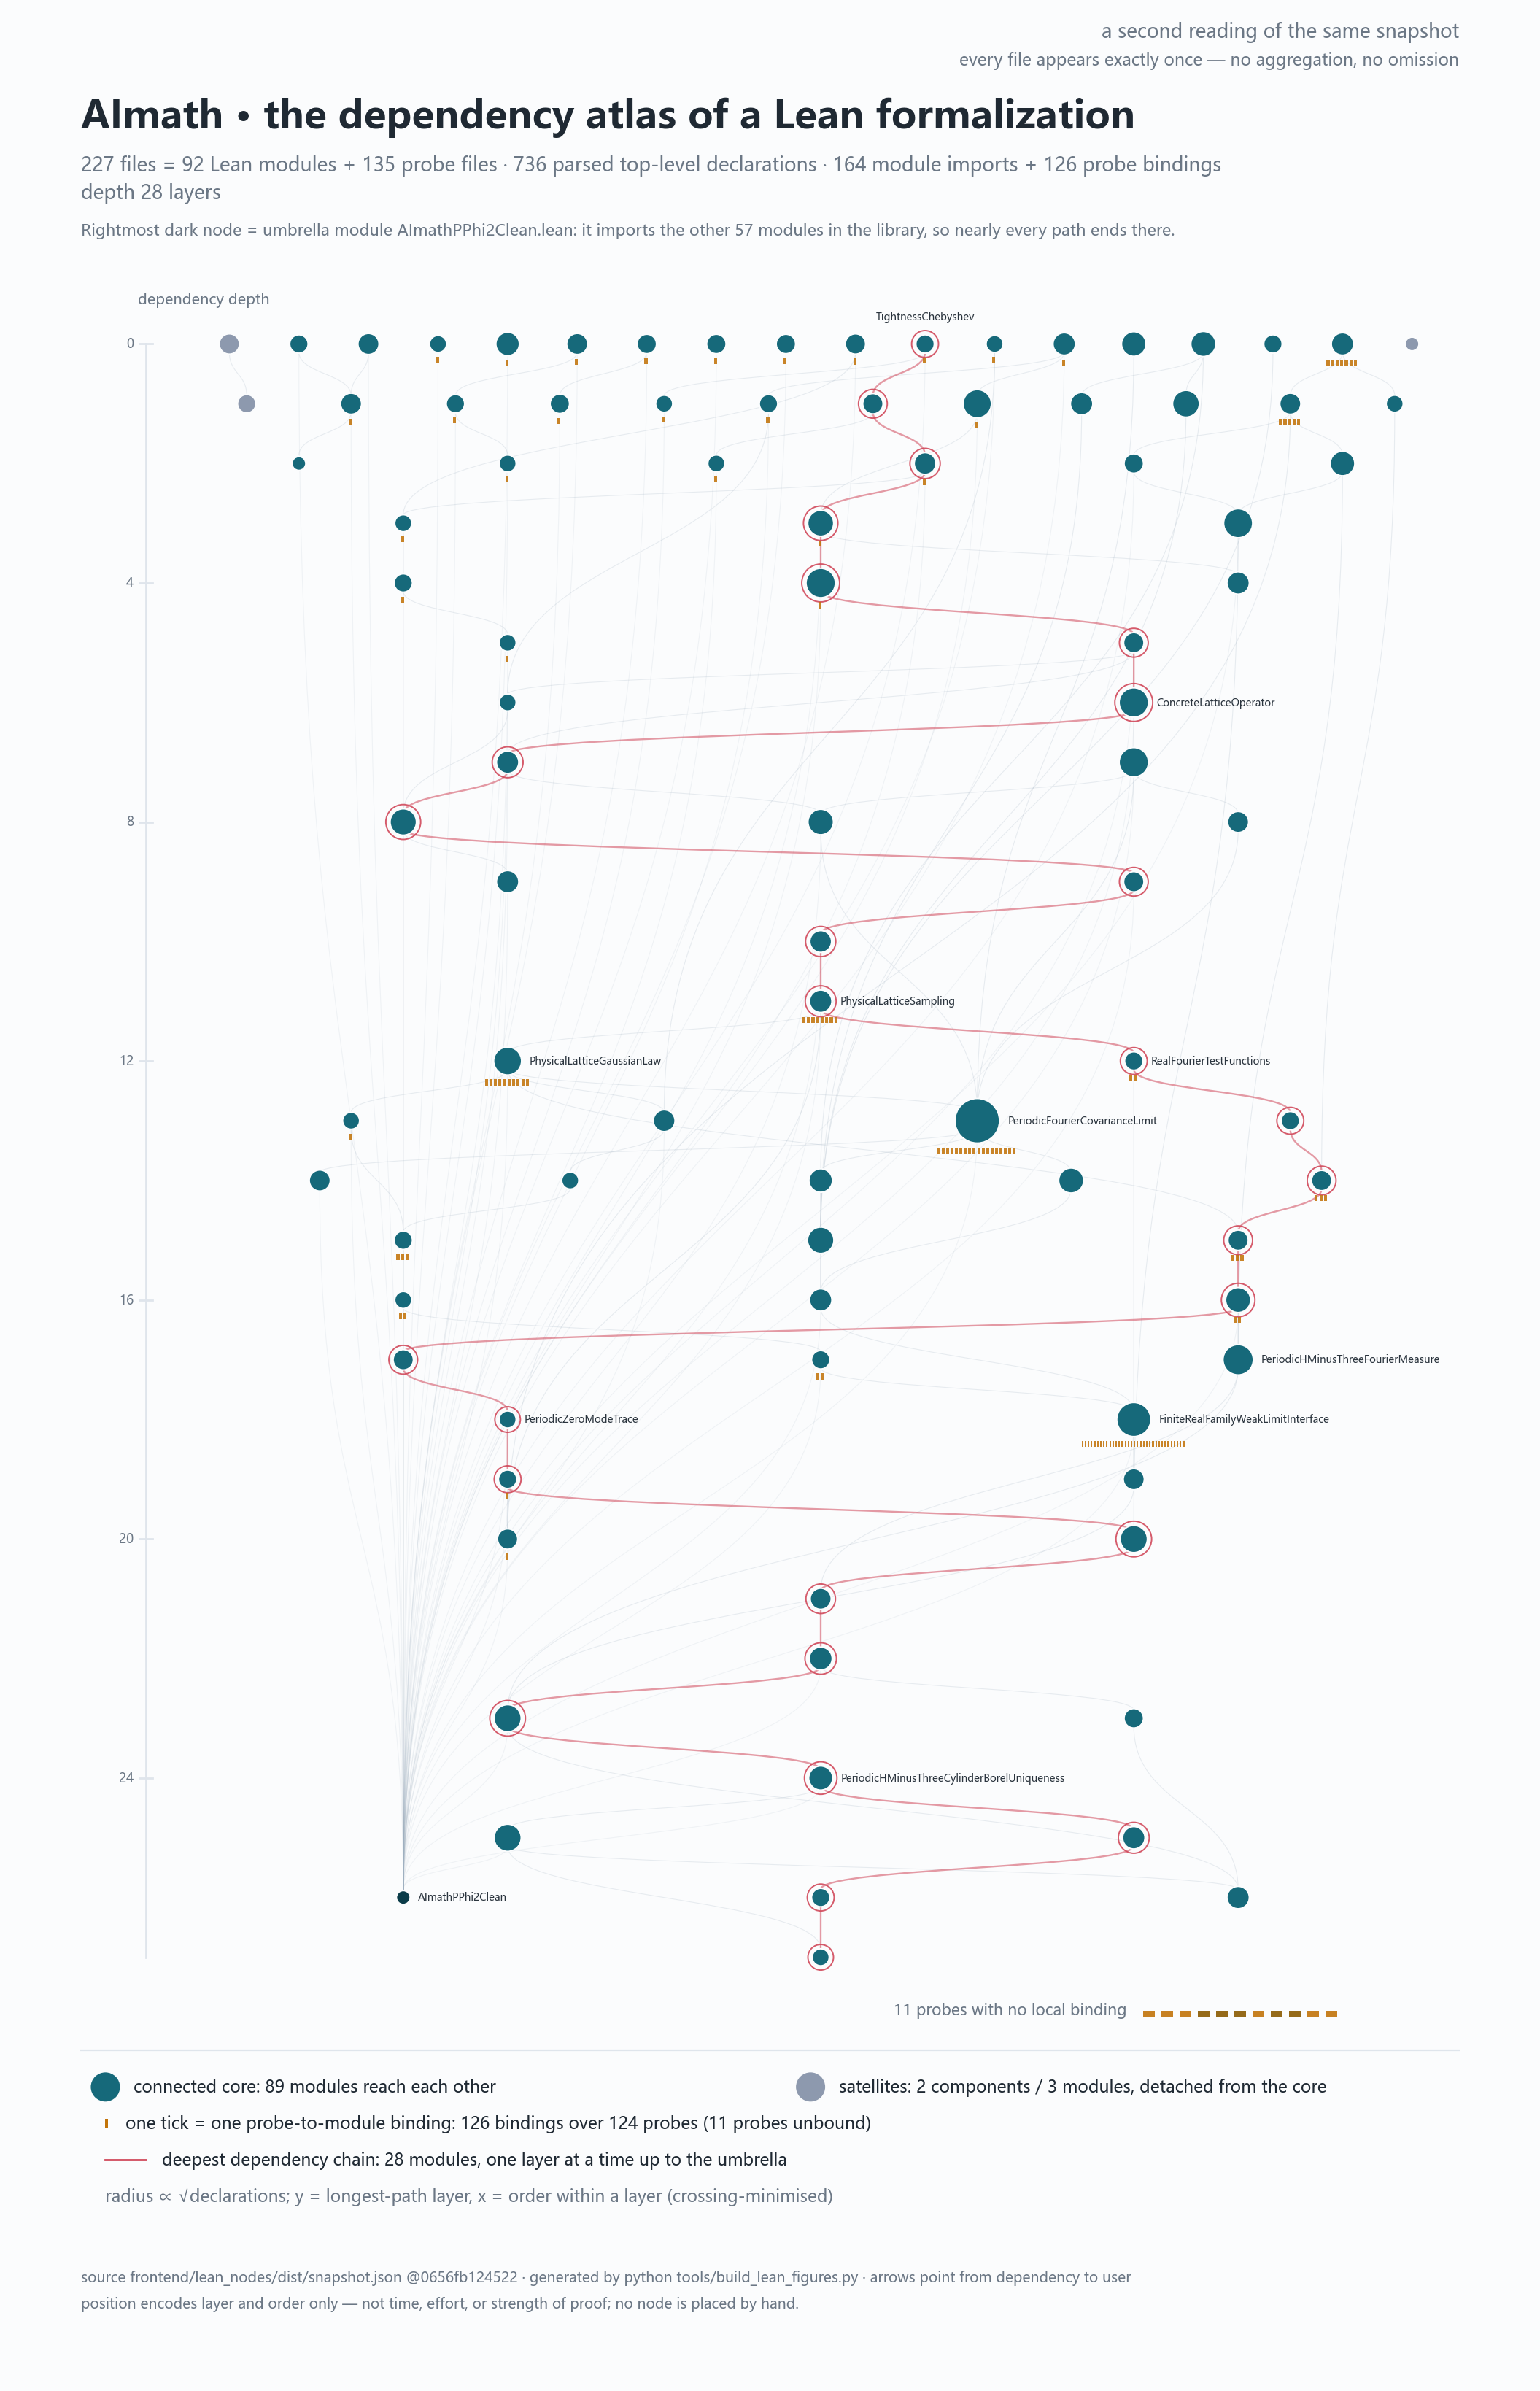
\includegraphics[width=0.62\linewidth]{figures/lean_atlas_en_portrait.png}
\caption{Dependency atlas of the Lean development. Each node is a module and each edge a declaration dependency. The atlas is a snapshot of a slightly wider tree than the package of \cref{sec:lean-overview}: it reports $92$ modules and $135$ probe files against the package's \NumCleanModules{} and \NumAuditProbes, and the figure's own legend identifies the three extra modules as satellites detached from the core rather than as part of it. The dense core the atlas names is the package. The surrounding directory of \cref{sec:lean-overview} is much larger than either count --- it holds \NumRootFiles{} further modules --- and none of it is drawn here. The figure is therefore best read as a picture of where the reported chain sits inside the tree that was measured, not as evidence about anything outside that chain.}
\label{fig:atlas}
\end{figure}
.
%
%  Each exclusion is stated with the reason it is a boundary of the statement
%  rather than a missing step: GAP R3 is item 1, GAP R4 item 3, GAP R7 item 4,
%  and the dimension restriction is item 5.
%
%  No priority claim is made, and no work is promised.  The citations are for
%  position only; the four structural points at the end are checkable in the
%  text and are not comparative.
%
%  Appendices are named in words rather than with \cref: their labels live in
%  main.tex, which the paper gate does not scan (same convention as W10).
% ==========================================================================
\section{Scope, boundaries, and the wider programme}\label{sec:scope}

Let $L>0$ and $m>0$.  \Cref{thm:main} proves that the finite-source Fourier
pushforwards $\mu_N$ of the fixed-volume lattice Gaussian laws converge weakly, as
a whole sequence, to the single Borel probability measure on the carrier
$\mathcal C=\HL{3}$ that their finite Fourier marginals determine. Its hypotheses
are proved in the same chain and not assumed: the tightness of the family
(\cref{thm:tightness}), with the uniform $\HL{2}$ moment behind it, and the limits
of the finite-marginal laws (\cref{thm:finite-family}), whose target is the paired
cosine and sine Gaussian law of the periodic resolvent.  Separately,
\cref{thm:covariance-limit} proves the analytic limit: the covariance integrals of
the physical lattice laws $\mu^{\mathrm{GJ}}_N$ converge to the pairing with the
resolvent of \cref{lem:resolvent}.  This section does the
opposite job.  It records what neither statement asserts, places what they do
assert among the branches of the programme, and points to the machine-checked
layer.

\subsection{What the paper does not assert}

Five boundary statements belong in the body rather than in a footnote: a reader who
supplies one of them from context would read the paper as claiming more than it
proves.  Each carries the reason it is a boundary of the statement, not a gap in
its proof.

\begin{enumerate}
\item \emph{What converges is the law of the Fourier coefficients.}  The
  sequence in \cref{thm:main} is $\mu_N=(L_N)_*\,\mu^{\mathrm{GJ}}_N$ of
  \cref{def:finite-source-lift}, and \cref{lem:lift-representative} identifies
  this as the law of a Borel carrier-valued map of the lattice Gaussian field.
  So the theorem does concern the lattice field laws; what it does not touch is
  any total lift specified independently of $L_N$ --- in particular the
  series-defined lift of the development, which carries its own measurability
  input (\cref{rem:lift-development}) --- and it says nothing about the field as
  a distribution on $\Torus$.  ``The lattice field laws converge'' is therefore
  asserted in the sense of the law of the coefficient sequence, which is the
  sense in which $\mu_N$ is a measure on $\mathcal C$ at all.
\item \emph{No identification with a distribution-defined Sobolev space, and no
  Laplacian domain theorem.}  The carrier is the explicit weighted $\ell^2$
  space of \cref{def:carrier-hminus3}, and \cref{prop:completion} is a statement
  about it: isometrically $\ell^2$, with $\HL{2}$ sitting inside continuously.
  The paper does not assert that $\mathcal C$ agrees with a Sobolev space of
  distributions defined independently of it, and it proves no strong domain
  theorem for an unbounded Laplacian.  Every estimate here is a weighted sum over
  modes, and no step is taken over from such an identification.
\item \emph{No covariance operator on the carrier, and no operator-level
  Gaussianity.}  The resolvent $R$ of \cref{lem:resolvent} is constructed on the
  $L^2$ space of the torus, not on $\mathcal C$, and no covariance operator is
  constructed on $\mathcal C$ here.  What is proved is the marginal statement of
  \cref{thm:main}(ii): for each finite tuple $F$ of modes, $(\Pi_F)_*\mu_{\mathrm{free}}$
  is the paired cosine and sine Gaussian law of \cref{thm:finite-family}.  Read
  as an operator statement, the proposition that $\mu_{\mathrm{free}}$ is the
  Gaussian measure whose covariance operator is $(m^2-\Delta)^{-1}$ is therefore
  not asserted.  A reader who wants it must either construct the operator on the
  carrier or use cylinder determination, since the cylinders generate the Borel
  sigma algebra (\cref{thm:cylinder-borel}) and the marginals determine the
  measure (\cref{thm:cylinder-uniqueness}).  It is listed here because it is a
  step this paper does not take.
\item \emph{No rate, no exponential tail, no modulus of continuity.}  Tightness
  (\cref{thm:tightness}) is Markov's inequality applied to the single first
  moment of \cref{thm:uniform-moment}, plus compactness of $\HL{2}$ sublevel
  sets in the weaker topology (\cref{thm:compact-tail}).  No exponential moment
  and no layer-cake argument enters, so no rate in $N$, no exponential bound on
  tail probabilities and no modulus of continuity for $\mu_{\mathrm{free}}$ is
  asserted.  A second moment of the norm is what \cref{ext:prokhorov} consumes through tightness, and nothing
  more.
\item \emph{The measure limit is two-dimensional.}  The mode lattice $\Z^2$, the
  weights $w_2,w_3$, the cylinder maps, the carrier and the law sequence are all
  two-dimensional, so \cref{thm:main} is a theorem about the two-dimensional
  carrier, and no dimensional generalisation of that carrier is claimed
  (\cref{rem:dimension}).  The covariance limit is the one statement whose
  source and machine-checked versions are registered for a general dimension
  $d$; Part~I writes the two-dimensional case that \cref{sec:setting} fixes.
  Nothing here says what becomes of the weights, the trace constant or the
  compact tail at $d\neq2$.
\end{enumerate}

\subsection{Where the result sits in the programme}

This paper is one step of one branch of a programme, and three other branches of
the same project are outside it.  Each is named so that a reader knows what this
paper is not about; none is evaluated, and nothing is promised.

\begin{itemize}
\item \emph{The free scalar theory in four dimensions} is the free massive
  Euclidean field on $\R^4$: the Gaussian measure on a space of distributions,
  its covariance, the Osterwalder--Schrader axioms for it, and the physics
  reconstructed from them.  This paper does not touch it; nothing here is stated
  on $\R^4$ or at infinite volume.
\item \emph{The interacting two-dimensional theory} is the $P(\varphi)_2$ model
  \cite{gjs1974}: interacting finite-volume laws, their ultraviolet limit at
  fixed volume, the axiom verification, and the mass gap.  This paper does not
  touch it; the laws whose covariance limit is \cref{thm:covariance-limit} are
  Gaussian at every mesh size.
\item \emph{The QED programme} is the non-perturbative construction of
  four-dimensional quantum electrodynamics, with its reconstruction and its
  physical content.  This paper does not touch it; no gauge-theoretic object
  occurs in the argument.
\end{itemize}

\begin{figure}[t]
\centering
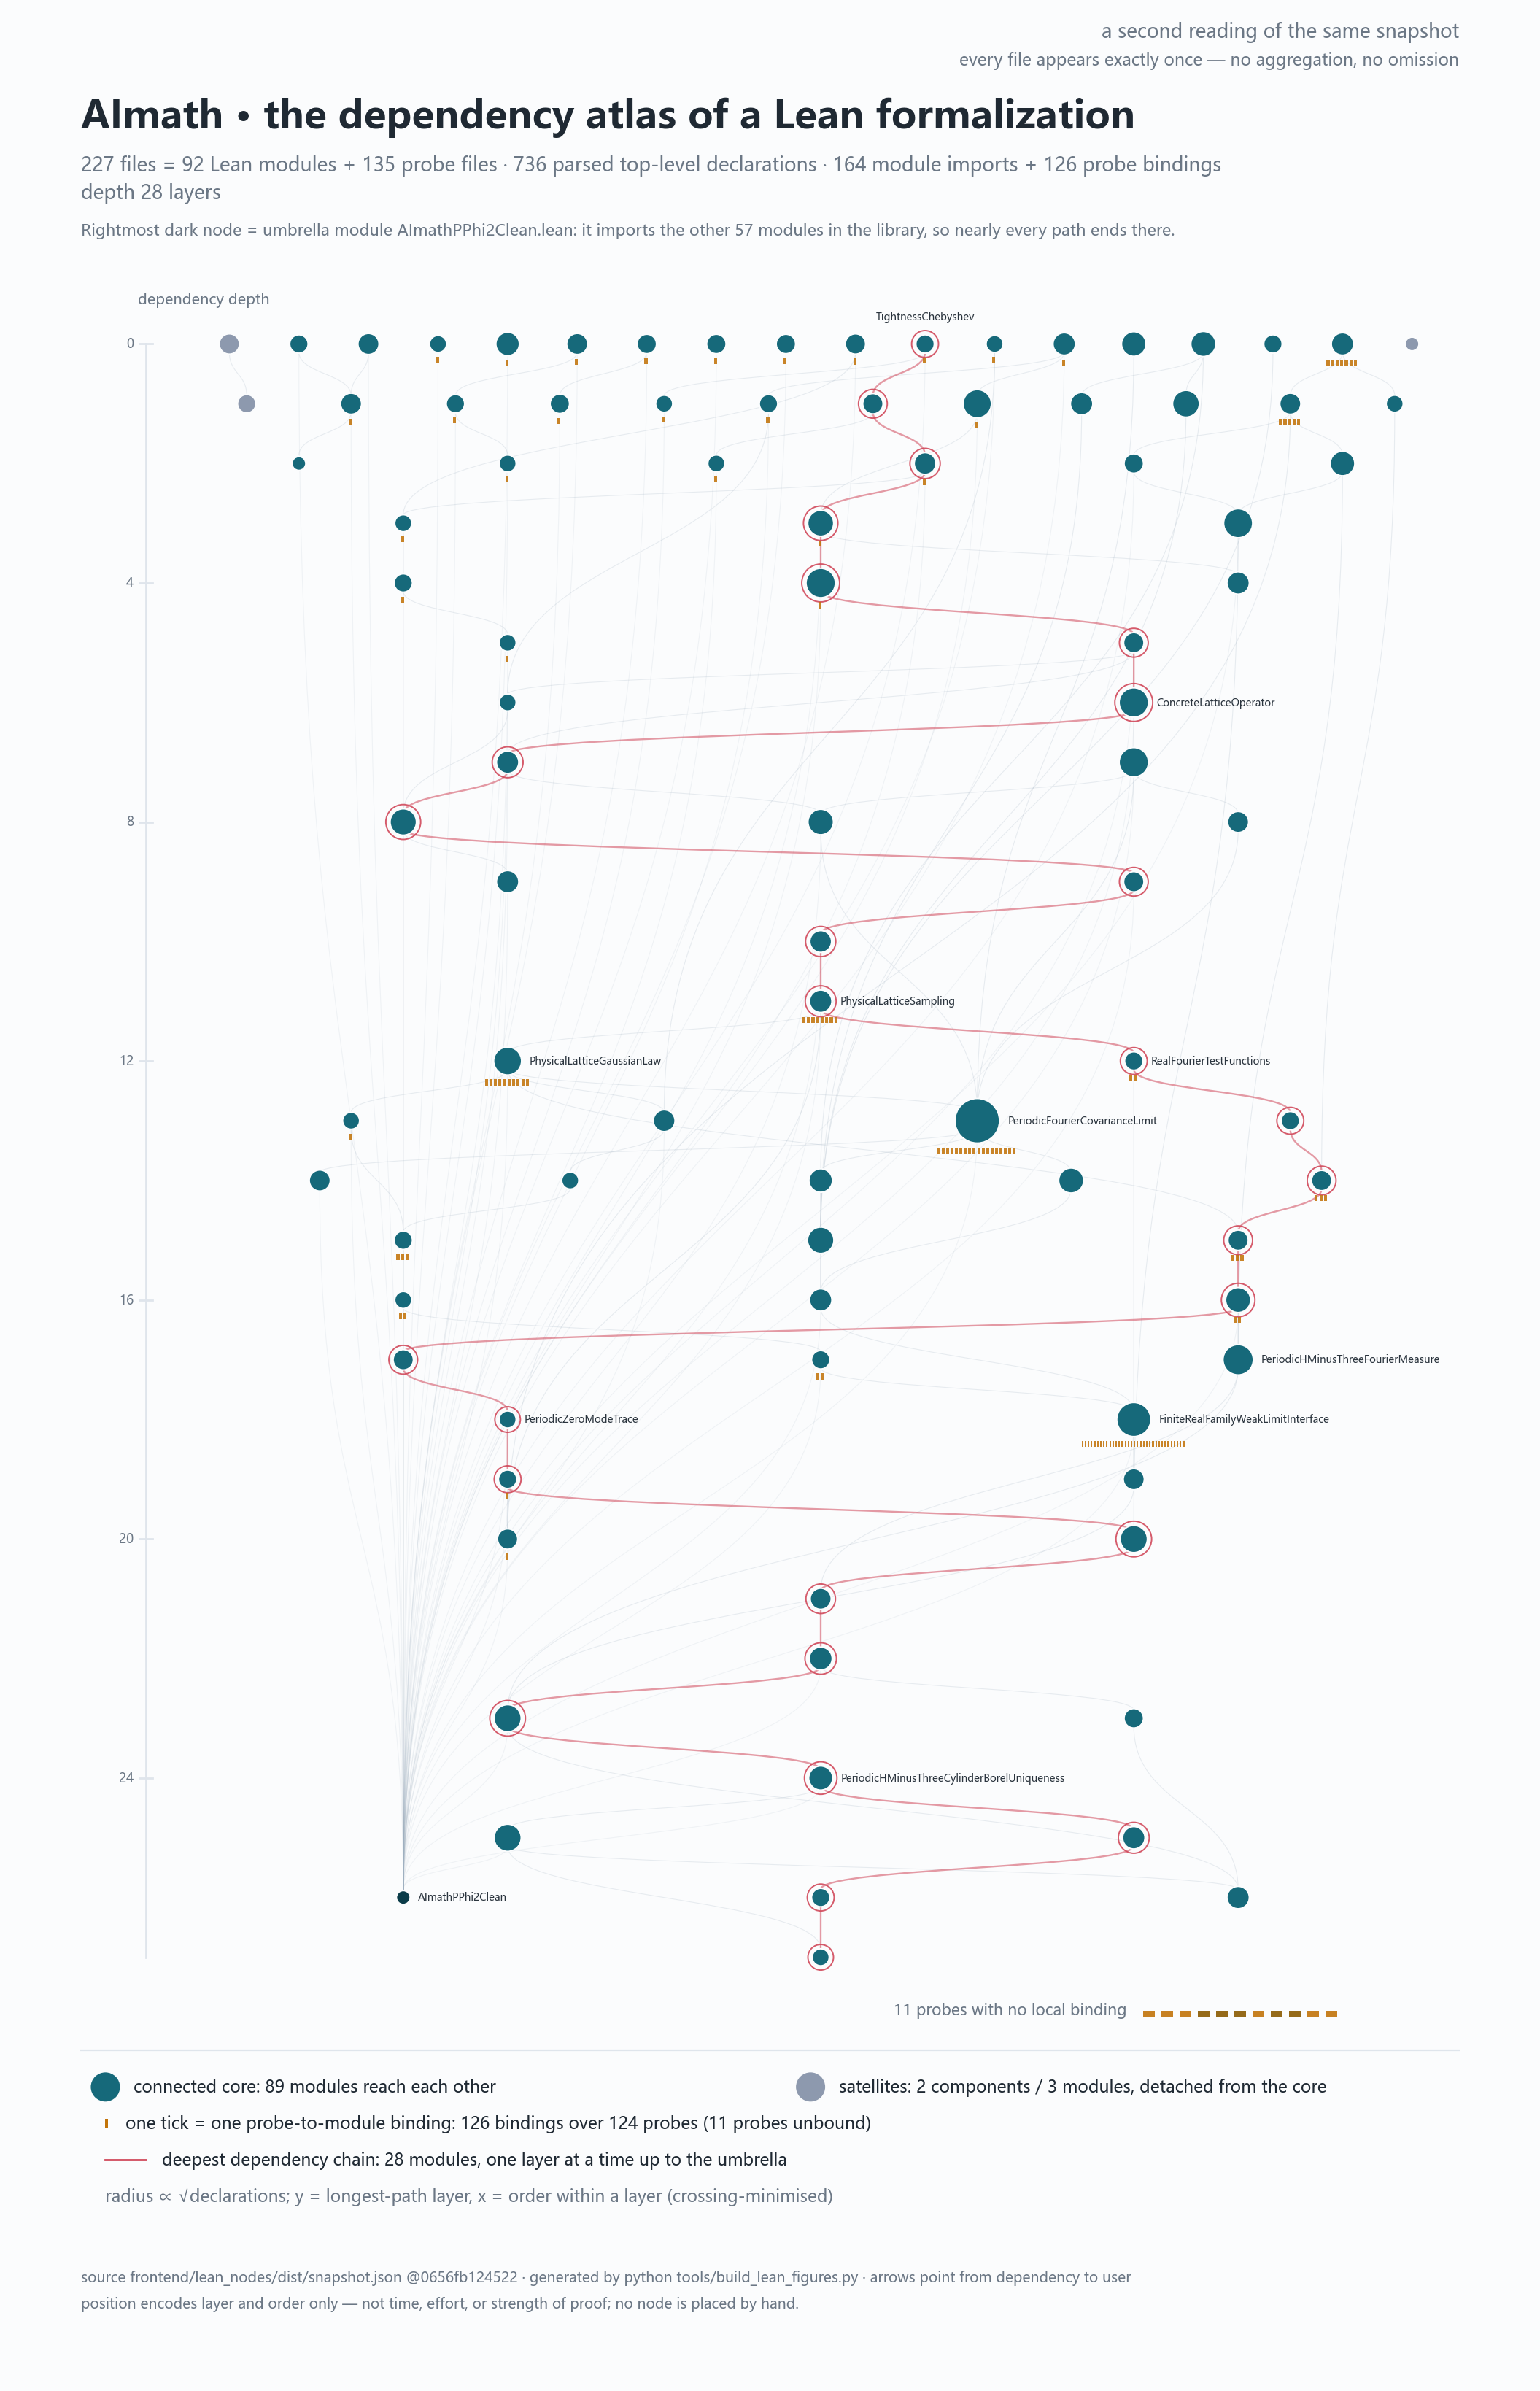
\includegraphics[width=0.62\linewidth]{figures/lean_atlas_en_portrait.png}
\caption{Dependency atlas of the Lean development. Each node is a module and each edge a declaration dependency. The atlas is a snapshot of a slightly wider tree than the package of \cref{sec:lean-overview}: it reports $92$ modules and $135$ probe files against the package's \NumCleanModules{} and \NumAuditProbes, and the figure's own legend identifies the three extra modules as satellites detached from the core rather than as part of it. The dense core the atlas names is the package. The surrounding directory of \cref{sec:lean-overview} is much larger than either count --- it holds \NumRootFiles{} further modules --- and none of it is drawn here. The figure is therefore best read as a picture of where the reported chain sits inside the tree that was measured, not as evidence about anything outside that chain.}
\label{fig:atlas}
\end{figure}


The atlas of \cref{fig:atlas} is a module-level dependency graph of the wider
Lean development of the project: its nodes are modules of that development as a
whole, not of the package this paper reports, and its edges are declaration
dependencies.  The package that Part~II reports is one cluster inside the atlas,
and the layers tabulated in \cref{sec:lean-overview} are the interior of that
cluster.

\subsection{Relation to the literature}

\NumCitedWorks{} works are cited in this paper, in two capacities that must not be
confused.  Four support a standard fact where it is used -- the Riesz
representation behind \cref{lem:resolvent}, the Prokhorov extraction of
\cref{ext:prokhorov}, the convergence of Gaussian laws with convergent
covariance matrices in \cref{thm:finite-family}, and the definition of weak
convergence on a metric space in \cref{rem:topology} -- and each is cited at that
point rather than here.  The remaining eight support nothing: they are cited
for position, and each of the following relations is a position, not a
dependency.  Seven of them are named below; the eighth, \cite{gjs1974}, is
named among the exclusions above.

\begin{itemize}
\item \cite{ossier1973,ossier1975} state the axioms: the properties
  (analyticity, reflection positivity, Euclidean invariance, clustering and
  regularity) that a Euclidean measure must satisfy before reconstruction can
  produce a Wightman theory.  They fix the target of the programme, and none of
  those properties is verified here.
\item \cite{gj1987} is the standard account of the programme as a whole, and so
  the reference point against which its order of steps is usually read; no step
  here is taken from it.
\item \cite{simon1974} and \cite{grs1975} are the monograph and the paper-length
  accounts of the two-dimensional model, and so the reference point for what a
  completed construction of that model contains; neither is used here.
\item \cite{nelson1973} is the reference point for the lattice Gaussian layer,
  the free Euclidean field and its Markov property, which is the layer the laws
  of \cref{def:gj-measure} belong to.
\item \cite{minlos1959} is the nuclearity and Minlos route from a
  positive-definite functional to a measure on the dual of a nuclear test space,
  which is the route this paper does not take: \cref{sec:carrier} builds the
  carrier as an explicit weighted sequence space, and \cref{ext:prokhorov} is
  the only extraction principle used.
\end{itemize}

Nothing above is a statement about priority.  The claim this paper makes about
its own result is structural, and each of its four parts is checked against the
text rather than against a comparison: the carrier is explicit
(\cref{def:carrier-hminus3}); the tightness is a single second moment of the norm
(\cref{thm:uniform-moment}); the limit is of the whole sequence and not of a
subsequence (\cref{thm:main}(i)); and the statements are formalised
(\cref{sec:lean-overview}).  Whether a comparable statement exists elsewhere,
and how it would compare if it did, is not established by anything here.

Part~II reports the machine-checked layer of the paper: \NumChainTheorems{}
declarations, from the covariance limit through the whole-sequence limit, with
\cref{sec:lean-overview} mapping each onto its module.  They are not uniformly
the same statements as Part~I, and where they differ the difference is in the
direction of weaker hypotheses or weaker conclusions, never stronger: the
finite-family declaration consumes as
a hypothesis the entrywise covariance identification that \cref{lem:hC-identification}
proves here, so what Lean closes is the passage from that identification to weak
convergence, not the identification itself.  How far coverage reaches is a
separate question with a separate answer, and \cref{sec:lean-boundary} is where
it is answered.


\part{The Machine Verification}\label{part:lean}

% ==========================================================================
%  Section 11 -- The Lean development: organisation and module map.  Owner: W09.
%  Frozen label: sec:lean-overview.  This is the first section of Part II.
%
%  Counts come from generated/metrics.tex only (CONTRACT section 6); no
%  structural count is typed here.  Every machine-checked name below is a
%  declaration of notes/lean_ledger.md section 2 (D12-D14, D30, D32, D42, D48,
%  D57, D58, D60, D61, D63); module names are set in \texttt, because a module
%  is not a declaration and must not be dressed as one.
%
%  Traps observed.  The root aggregator is not claimed to build every module
%  (CONTRACT section 11, final paragraph); the appendices are named in words
%  because their labels live in main.tex, which the paper gate does not scan.
% ==========================================================================
\section{The Lean development: organisation and module map}
\label{sec:lean-overview}

The formalisation is a separate Lake package, \lmod{AImathPPhi2Clean}, whose
sources live under \lmod{formal/lean/s6/pphi2_clean/}, built against Mathlib on
Lean \LeanToolchain{}. \lmod{lake-manifest.json} pins the Mathlib commit
\texttt{85e3a25e}, which is the revision of the tag \lmod{lakefile.lean} names. It has
\NumCleanModules{} modules and
\NumCleanLines{} lines of Lean, together with \NumAuditProbes{} audit probe
files; a comment-stripped count, computed at build time by the paper's own
script and never typed here, finds \NumCleanSorry{} \texttt{sorry} and
\NumCleanProjectAxioms{} project axioms in those modules. The library target
builds: \lmod{lake build AImathPPhi2Clean} elaborates all \NumCleanModules{}
modules with no error on the pinned revision, including the
\NumUnreachableModules{} that the root file does not reach
(\cref{sec:lean-boundary}).  The package sits
inside a larger development: the surrounding directory
\lmod{formal/lean/s6/} holds \NumRootFiles{} further modules with
\NumRootLines{} lines, which this paper does not take as its subject, does not count, and does
not claim to cover.  Every declaration quoted below lives in the namespace
\lmod{Pphi2Clean.Continuum}.

The modules are organised in layers, and the layers follow the order of the
conclusions rather than the order of the proofs: each
one exposes an interface that the next one consumes, so the map below is also a
reading order.  The entry module in the right-hand column is the module to open
first for that layer.

\begin{center}
\scriptsize
\begin{tabular}{@{}p{0.225\linewidth}p{0.325\linewidth}p{0.40\linewidth}@{}}
\toprule
Layer & What it does & Entry module(s) \\
\midrule
(a) periodic torus $L^2$/$H^1$ and the discrete operator &
  Periodic $H^1$ as a closed value-gradient graph completion; the finite
  periodic lattice, its discrete Laplacian with spacing $a$, and an eigenbasis
  of $Q=-\Delta_a+m^2$ &
  \lmod{PeriodicTorusH1}, \lmod{ConcreteLatticeOperator},
  \lmod{PeriodicFourierLaplacian} \\
(b) the massive resolvent and its energy solver &
  The weak massive resolvent from an energy form and a Riesz adjoint; sampled
  and continuum Fourier coefficients; the cutoff tail uniform in the mesh; the
  three covariance limits restated with the resolvent as target &
  \lmod{PeriodicFourierCovarianceLimit},
  \lmod{PeriodicTorusResolventLimit} \\
(c) physical lattice sampling and the Gaussian law &
  Sampling of a test at physical sites with the cell volume as weight; the
  normalised finite covariance; zero mean, characteristic function,
  mixed-moment identity, and the covariance-to-weak-convergence transfer &
  \lmod{PhysicalLatticeGaussianLaw},
  \lmod{PhysicalLatticeSampling} \\
(d) negative-Sobolev carriers, topology and Borel structure &
  The $\HL{2}$ and $\HL{3}$ weights, the completion as $\ell^2$ with its weight
  and deweight maps, the compact-tail comparison, the coordinate embeddings,
  second countability, separability, and the cylinder sigma algebra equal to
  the Borel one &
  \lmod{PeriodicHMinusThreeCompletion},
  \lmod{PeriodicHMinusThreeTopologyBorel} \\
(e) uniform $\HL{2}$ moment and $\HL{3}$ tightness &
  The trace of the squared $\HL{2}$ norm under the finite Gaussian source and
  its mesh-uniform bound; the extended energy, its compact sublevels, the Markov
  tail, and tightness of the law sequence &
  \lmod{PeriodicHMinusTwoUniformTightness},
  \lmod{PeriodicHMinusThreeFixedVolumeTightness} \\
(f) finite real families, characteristic functions and covariance convergence &
  The resolvent covariance matrix, its positive semidefiniteness and Gram
  factor, the canonical target Gaussian, and unconditional weak convergence for
  every finite family of tests &
  \lmod{FiniteRealFamilyWeakLimitInterface},
  \lmod{FiniteFourierCoordinateConvergence} \\
(g) cylinder convergence &
  All the lift maps, the finite-source measure, the paired cosine and sine
  cylinder family, and convergence of every finite Fourier marginal &
  \lmod{PeriodicHMinusThreeCylinderConvergence},
  \lmod{PeriodicHMinusThreeFourierMeasure} \\
(h) Prokhorov subsequence &
  Tightness in the form Prokhorov consumes, and a strictly monotone subsequence
  converging to a Borel probability measure on the carrier &
  \lmod{PeriodicHMinusThreeProkhorovSubsequence} \\
(i) cylinder-to-Borel uniqueness &
  Finite-coordinate cylinders as a $\pi$-system, the Borel-generation step
  discharged from separability, and equality of two Borel probability measures
  with equal indexed cylinder marginals &
  \lmod{PeriodicHMinusThreeCylinderBorelUniqueness} \\
(j) final assembly &
  Inheritance of the target marginals by any subsequential limit, existence and
  uniqueness of the whole-sequence limit, and the packaged
  existence-with-cylinders statement &
  \lmod{PeriodicHMinusThreeWeakLimitMarginal} \\
\bottomrule
\end{tabular}
\end{center}

Layers (a) and (b) are analysis on the torus, layers (c) to (e) are the lattice
laws together with the carrier and the single moment, layers (f) to (i) are the
convergence and identification steps, and layer (j) applies them in order.

The correspondence with Part~I is by result, not by proof step.  Every name in
the right-hand column lives in the namespace \lmod{Pphi2Clean.Continuum} and
the namespace is omitted there.  \Cref{app:ledger} lists the
\NumChainTheorems{} declarations frozen in the two statement contracts, with the
module that declares each of them; the remaining names of the table below are
declarations of the same package whose role is described here rather than
frozen, and their existence is checked against the Lean sources by the paper's
own gate rather than against the registry.

\begin{center}
\footnotesize
\begin{tabular}{@{}p{0.16\linewidth}p{0.82\linewidth}@{}}
\toprule
Result in Part~I & Declaration(s) in \lmod{Pphi2Clean.Continuum} \\
\midrule
\cref{thm:covariance-limit} &
  \lean{fixedVolumeCovarianceInner_tendsto_torusFourierGreenPairing}\newline
  \lean{physicalGJMeasure_fixedVolume_mixedMoment_tendsto_torusFourierGreenPairing}\newline
  \lean{physicalGJMeasure_fixedVolume_covariance_tendsto_torusFourierGreenPairing} \\
\cref{thm:separable} & \lean{periodicHMinusThreeCompletion_separable} \\
\cref{thm:cylinder-borel} &
  \lean{periodicHMinusThree_cylinder_sigma_eq_borel_of_polish} \\
\cref{thm:tightness} &
  \lean{periodicHMinusThree_fixedVolume_freeField_tight} \\
\cref{thm:finite-family} &
  \lean{physicalFamilyEvalProbabilityMeasure_fixedVolume_weak_tendsto_of_periodic_fourier_canonical} \\
\cref{thm:cylinder-uniqueness} &
  \lean{periodicHMinusThree_probabilityMeasure_ext_of_indexed_cylinder_marginals} \\
\cref{lem:subsequence-marginals} &
  \lean{periodicHMinusThree_weak_limit_has_expected_cylinder_marginal}\newline
  \lean{periodicHMinusThree_fixedVolume_subsequential_limit_has_expected_cylinder} \\
\cref{cor:uniqueness} &
  \lean{periodicHMinusThree_fixedVolume_weak_limit_unique} \\
\cref{thm:main} &
  \lean{periodicHMinusThree_fixedVolume_weak_limit_exists_with_expected_cylinders}\newline
  \lean{periodicHMinusThree_fixedVolume_weak_limit_exists}\newline
  \lean{periodicHMinusThree_fixedVolume_weak_limit_has_expected_cylinder} \\
\bottomrule
\end{tabular}
\end{center}

For the \NumChainTheorems{} declarations of the chain the correspondence is
statement by statement: each of the nine results in the left-hand column has at
least one declaration on its right whose conclusion is that statement, and the
three limits inside \cref{thm:covariance-limit} are the three declarations of the
first row, one per line of that theorem.  Two rows carry a qualification, and
they are the two the reader is most likely to overread.
The finite-family declaration consumes the entrywise covariance identification as
a hypothesis --- that is, the very statement \cref{lem:hC-identification} derives
from the covariance limit --- so what the machine closes there is the passage from
that identification to weak convergence of the finite families, with the target
supplied by the Fourier-constructed factor.  The covariance input is exactly
what \cref{thm:finite-family} does not assume, because Part~I spends
\cref{sec:covariance} proving it.
The cylinder-Borel declaration is stated under a Polishness input rather than
unconditionally, and the same module derives that input from separability of the
carrier (\lmod{periodicHMinusThreeCompletion_separable}), which is how the chain
that consumes it discharges it; Part~I's version is unconditional because
\cref{sec:carrier} proves separability before stating it.  Neither qualification
makes a row claim more than Part~I does.
That is the precise
sense in which Part~II mirrors
Part~I, and it is what the table lets a reader check without reading Lean: the
paper's statement on the left, the declaration that carries it in the middle
column, and the module that declares it in Appendix~A.  The row for
\cref{cor:uniqueness} is the weakest entry in the table and must be read as
such: the declaration it names says that two limits of one filter coincide,
which is Hausdorff uniqueness of a filter limit, and not that the limit is
characterised.  The characterisation is the cylinder rows of the table, as it is
in Part~I.  What the table does not
say is anything about the three parts of \cref{thm:main} separately: existence
and the marginal statement are carried by the three declarations of the last row,
while part~(iii), the uniqueness of the limit, is carried by the
cylinder-uniqueness row above it --- that row's declaration is the formal
counterpart of Part~I's part~(iii), though Part~I states no Lean name.

Two qualifications belong here rather than in a footnote, because a reader who
misses either will overread the table.  First, the formal development is a
separate unit from this paper's prose: it has its own module structure, its own
definitions and its own conventions for normalisation, so the package is not the
paper transcribed, and the paper does not claim that the Lean code follows the
proof of Part~I line by line.  Statement identity is what is on offer here, and
it is all that is on offer.  Second, coverage is not uniform across the layers,
and \cref{sec:lean-boundary} collects the five places where the development
diverges from a maximally favourable reading of it: which modules the package
root reaches, a final-theorem-shaped wrapper that assumes its own conclusion,
the total-lift measurability input that is not proved, the two-dimensional
restriction of the measure chain while the covariance theorems are stated for
general dimension, and what a complete build does and does not establish.

Part~II's two appendices are ordered accordingly.  Appendix~A
(\cref{app:ledger}) is the declaration ledger and Appendix~B
(\cref{app:axioms}) the axiom-footprint transcript, and both are generated on
every build from the statement registry and from the recorded transcript rather
than typed, because a hand-maintained list of declaration names is exactly the
kind of object that goes stale without anyone noticing.

% ==========================================================================
%  Section 12 -- Statement contracts and the axiom firewall.  Owner: W10.
%  Frozen label: sec:lean-contracts.
%
%  Sources read for this section: formal/lean/challenges/_registry.yaml (the
%  two entries PPHI2_FIXED_VOLUME_COVARIANCE_LIMIT and
%  PPHI2_FIXED_VOLUME_FREE_FIELD_MEASURE_LIMIT, and permitted_axioms),
%  the per-node <NODE>.hashes.json digest files, tools/lean_challenge.py
%  (the runner), and ext/axiom_transcript.txt.
%
%  Traps observed here.  (a) CONTRACT section 11: a SKIP is not a pass, so
%  the remote_only paragraph says so in its first sentence and again at its
%  end.  (b) A footprint is a statement about dependence, never about the
%  intended statement; the last subsection keeps the two roles apart.
%  (c) The appendix labels are declared in main.tex, which the paper gate
%  does not scan for labels, so the appendices are named in words rather
%  than cross-referenced with \cref.
% ==========================================================================
\section{Statement contracts and the axiom firewall}\label{sec:lean-contracts}

Two devices carry the discipline of the formal side, and neither of them is a
proof: a \emph{statement contract}, which fixes what is to be proved, and an
\emph{axiom firewall}, which bounds what the proof of it may assume. This
section describes both, and separates what each establishes from what it leaves
open; the divergences that remain are the subject of \cref{sec:lean-boundary}.

A statement contract is an entry of the statement registry of the development,
\lmod{formal/lean/challenges/_registry.yaml}. For one node of the development
it freezes three things: the modules of the delivered package that declare the
results, the theorem names in fully qualified form, and a digest of each
statement, held beside the entry in a per-node file. The registry carries
\NumContracts{} contracts. The two this paper reports are
\lmod{PPHI2_FIXED_VOLUME_COVARIANCE_LIMIT} and
\lmod{PPHI2_FIXED_VOLUME_FREE_FIELD_MEASURE_LIMIT}. The first freezes
the covariance declarations, among them
\lean{fixedVolumeCovarianceInner_tendsto_torusFourierGreenPairing}; the second
freezes the measure-limit declarations, among them
\lean{periodicHMinusThree_fixedVolume_weak_limit_exists}. ``Fully qualified''
means that the namespace is part of the frozen string: each of the
\NumChainTheorems{} names this paper reports lives in
\lmod{Pphi2Clean.Continuum}, and the ledger of Appendix~A omits that prefix
only because the omission is itself performed mechanically.

\subsection{What freezing buys}

The digest is taken of what Lean prints for \texttt{\#check @} of a name, that
is, of the elaborated type with all implicit and instance binders, not of the
source text as typed. A later strengthening, weakening or reparametrisation of a
statement therefore produces a different digest. The runner reports the mismatch
and refuses the statement; it does not overwrite the recorded value, so the
contract stays red across runs, and the only way past it is to record the new
statement together with a written reason. That is what freezing buys: a
statement cannot change quietly, and a change accepted once cannot become
invisible afterwards.

\subsection{Both contracts are remote-only}

Both entries are marked remote-only and name the separate Lake project that hosts
the recorded digests, \lmod{/home/zhengyj/AImath-lean/AImathPPhi2Clean}. The
runner reads that field before it does anything else, and reports \lmod{SKIP} with
the declared project as the reason. \textbf{A \lmod{SKIP} is not a pass.} It
records that the digest was neither confirmed nor refuted locally, because the
recorded values live beside that project; a reader who takes the absence of a
failure for a success reads the output backwards. The flag is about \emph{where
the digest runner points}, not about whether the package can be elaborated: the
package is in this repository and, as \cref{sec:lean-overview} and the
reproduction section record, it builds in place. The evidence standing behind
these two contracts is therefore two-part: the digests and the registry entry on
the project side, and, on this side, the transcript of Appendix~B, produced by
building the modules that declare the \NumChainTheorems{} theorems and elaborating one audit file
against them.


\subsection{The axiom firewall}

The permitted set of the development is \NumPermittedAxioms{} names, the axioms
of the Lean kernel and of \lmod{Mathlib}:
\[
  \lmod{propext},\qquad \lmod{Classical.choice},\qquad \lmod{Quot.sound}.
\]
Every declaration this paper reports has
been checked with \texttt{\#print axioms}; each contract's check file issues that
command once per frozen name, next to the \texttt{\#check} that produces the
digest, so one file exercises both devices. This paper reports
\NumChainTheorems{} declarations, and the footprint of every one of them is equal
to the permitted set: no axiom introduced by the project appears, and no
placeholder standing for an omitted proof appears. Two thresholds are in force
and they are not the same one. The contract runner refuses a footprint that
contains any name outside the permitted set. The generator of Appendix~B applies
two further rules of its own: it refuses a transcript that is empty, that is not
tab-separated, whose rows are not all equal to one another, or any of whose rows
leaves the permitted set. The equality with the permitted set \emph{as a set} is
enforced one step later, by the paper's own gate, which is why a footprint that
merely stayed inside the permitted set would not reach this paper.

\subsection{The negative control}

A test that has never failed has not been shown to be able to fail. The package
therefore ships a probe, \lmod{audit/negative_axiom.lean},
\NumNegativeControlLines{} lines long: it injects
\texttt{axiom injectedAxiom : False}, derives
\texttt{theorem polluted : False := injectedAxiom}, and prints the footprint of
the derived theorem, and one line of its run output records a footprint carrying
the injected axiom and none of the permitted three. What that
establishes is that the footprint test has a case in which it must fail, so a
green run of it is not an artefact of a check that can only say yes. What it does
not establish is anything about any particular declaration: the probe is a
separate file, it is not a perturbation of the frozen names, its recorded output
is a bare measured line rather than a transcribed session with commands and a
date, and it exercises the footprint test only, not the digest. The control is
therefore attested textually -- the file is in the tree and its output line is
committed beside it -- and not by a transcript of the standard of Appendix~B.

\subsection{Two roles: dependence and intent}

A footprint is a statement about dependence, and dependence is not content.
Equality with the permitted set says that the proof term of the declaration uses
no axiom outside that set; it says nothing about whether the statement is the
intended one, because the footprint is read off the proof term and the shape of
the statement is not part of what it records. A declaration that proves a weaker
proposition, or a different one, has the same footprint as a declaration that
proves the intended proposition. What addresses intent is the other two devices.
The digest of the contract detects a change in a statement over time, and the
ledger of Appendix~A fixes, for every reported declaration, its module and its
role in the argument. The division of labour is therefore: the firewall reports
what was assumed, the digest reports what was frozen, the ledger reports where
the declaration sits. All three are necessary, none is sufficient, and what the
three together still leave unchecked is stated in \cref{sec:lean-reproduction}.

% ==========================================================================
%  Section 13 -- What is machine-checked and what is not.  Owner: W10.
%  Frozen label: sec:lean-boundary.
%
%  Architecture: a numbered list of divergences, each a fact about the sources,
%  with no qualifier that softens it.  Every item is backed by notes/lean_ledger.md
%  sections 4 and 5; the counts that exist as macros are macros, the reachability
%  count is the word "eight" (CONTRACT section 11, final paragraph), and the direct
%  import count is deliberately not stated (it would be a typed structural count).
%
%  Traps observed here.  (1) The root aggregator does not build every module, and
%  the footprints of six registered theorems rest on the transcript, not a build.
%  (2) The final-theorem wrapper proves nothing; it may be named, and must be
%  called vacuous in the same breath.  (3) The total-lift zero convention is not a
%  null-set assertion; the chain avoids it.  (4) The measure chain is 2-dimensional
%  while the covariance theorems are general-d.
% ==========================================================================
\section{What is machine-checked and what is not}\label{sec:lean-boundary}

The formal side of this paper is easier to overstate than to state, so the
divergences between the sources and a maximally favourable reading are collected
here as numbered facts. Each is a property of the sources, not a hedge on a
result: the declarations asserted below are the declarations that exist, and the
sentences below say how far the evidence for them extends. The influence of each
item on the mathematics is none; the influence on what a reader may conclude is
total.

\begin{enumerate}

\item \emph{Reachability.} \NumCleanModules{} modules exist in the package, and
  the package root aggregator imports a subset of them directly.
  \NumUnreachableModules{} modules are not reachable from the root file even
  transitively. Two of them are load-bearing:
  \lmod{PeriodicHMinusThreeWeakLimitMarginal}, which declares
  \NumUnreachableChainTheorems{} of the \NumMeasureContractTheorems{} registered
  measure-limit theorems, and
  \lmod{PeriodicHMinusThreeProkhorovSubsequence}, which declares the Prokhorov
  extraction step of the argument. Consequently a build of the \emph{root file}
  does not evidence the axiom footprints of those declarations: nothing reachable
  from it contains them, so a claim that the root covers the development is a
  claim about a subset of the package. What does evidence them is a build of the
  library target, which elaborates every module including the unreachable ones,
  and that is the build Appendix~B records. The distinction matters to a reader
  who builds the aggregator and stops: the result is green and says nothing about
  \NumUnreachableModules{} modules, \NumUnreachableChainTheorems{} of whose
  declarations are on this paper's chain.

\item \emph{A vacuous wrapper.} The development contains a
  final-theorem-shaped interface,
  \lmod{latticeFreeFieldMeasure_tendsto_periodicFreeGaussian}, whose proof is
  \texttt{exact hfinal}: it assumes its own conclusion. This paper does not use
  it, and no result on these pages depends on it. It exists as a contract-shaped
  interface, listing the data that a completed assembly would have to supply --
  tightness, the finite marginals, the cylinder-to-Borel input and the
  subsequential identification -- and a reader who found it by its name and its
  shape would take it for the paper's theorem. It is not, and citing it as such
  would be filing an empty citation.

\item \emph{The formalisation's lift is not the paper's}. The development's
  carrier-valued lift is a total function, defined coordinatewise with the
  series appearing only in the $\ell^2$ side condition, together with the
  convention that it is $0$ off the convergence set; its measurability is one
  conjunct of an input of the formal development, the other conjunct asserting
  almost-everywhere agreement with the raw weighted lift. That convention is
  \emph{weaker} than a range statement and must not be read as one: the function
  is total at the price of the convention, not of a theorem about it. Nothing in
  the mathematics turns on it. The paper's carrier-valued representative is $L_N$
  of \cref{def:finite-source-lift}, whose total range, Borel measurability and
  entry formula are proved outright (\cref{lem:lift-representative}), and the
  chain of \cref{sec:main} runs through $L_N$, not through the development's
  lift; on the finite-source route the development moreover proves the two
  pushforwards equal without using the input. So a
  reader comparing the two sources should read the development's input as a fact
  about one implementation choice, not as a gap in \cref{thm:main}. What is
  genuinely absent on both sides is stated in \cref{sec:scope}.

\item \emph{Dimension.} The measure chain is hard-wired to two dimensions: the
  carrier, the Fourier index set, the cylinder maps and the law sequence are all
  built over the two-dimensional index set, and no parameter for the dimension
  occurs in them. The registered covariance theorems are stated for a general
  dimension $d$. The two statements are therefore not the same statement
  generalised differently: the covariance statements are \emph{registered} for
  general $d$ (that is how the Lean declarations quantify), this paper writes
  them in $d=2$, and the measure limit, as formalized, is available in $d=2$
  only. No dimension other than two is claimed anywhere in Part~I
  (\cref{rem:dimension}).

\item \emph{What a green build proves.} A complete build proves the Lean
  declarations that the sources state, under the hypotheses that the sources
  attach to them, on the toolchain recorded in the transcript; a complete build
  of this package exists and is recorded in \cref{sec:lean-reproduction}. It
  proves nothing
  about the mathematics of a hypothesis: a hypothesis is an input, and a build
  that consumes it is not evidence for it. It proves nothing about statements
  outside the library target of Item~1. And the count of \NumCleanSorry{}
  occurrences of \texttt{sorry} is a statement about the text of the sources,
  obtained by a scan that strips comments, rather than a statement about the
  mathematics: a source file free of placeholders can still formalize a
  proposition weaker than the one a reader has in mind, which is why Item~3 and
  Item~4 are stated here rather than absorbed into the count. The mathematical
  boundary of this paper -- the coverage comparison between these ten
  declarations and the rest of the development, and the absence of a rate -- is a
  different boundary, and \cref{sec:scope} draws it.

\end{enumerate}

% ==========================================================================
%  Section 14 -- Reproduction.  Owner: W10.
%  Frozen label: sec:lean-reproduction.
%
%  Sources read for this section: build_all.py (steps 1-7), audit/count_lean.py,
%  audit/make_ledger.py, audit/make_bib.py, audit/verify_paper.py (the four checks
%  N/E/L and their negative controls, the docstring "known limits"), main.tex
%  (the two documented build commands) and ext/axiom_transcript.txt lines 8-18
%  (the two recorded commands).
%
%  Traps observed here.  (a) No build-job count and no wall-clock time is stated:
%  both are environment-dependent and would rot.  (b) The reproducibility claim is
%  limited to declaration names and frozen digests; the correspondence of a paper
%  sentence with a Lean statement is not machine-checked and is said so.
% ==========================================================================
\section{Reproduction}\label{sec:lean-reproduction}

Two entry points are supported and they are not equivalent. The paper's own gate
is \texttt{python build\_all.py}, run from the paper directory. In order it
regenerates the structural counts and both appendices -- the declaration ledger
from the sources, the axiom transcript from the recorded engine output -- runs the
negative controls of the paper checks and then the checks themselves, compiles
with Tectonic \TectonicVersion{}, refuses a PDF older than any source, and stamps
the digest of every source and of the output into \lmod{build/LAST_BUILD.txt}.
The four checks are: that every Lean name quoted in the body is a name the
generated ledger lists, or else a declaration of the package found in the Lean
sources; that the large structural counts in the body are macros rather than
typed values; that labels, cross-references, citations and bibliography
keys close and every section carries a label; and that the axiom story is
self-consistent, in the sense of \cref{sec:lean-contracts}. Stated precisely: the
count check rejects a typed literal only when the macro it should have used has
at least three digits or a value of at least forty, so a hand-typed
\texttt{two} would pass it, and the discipline for small numbers is editorial
rather than mechanical; the check also fails when a macro that the build computes
is quoted nowhere, which is the failure mode a typed count leaves behind. The
reference check covers every reference command the document uses, \verb|\eqref|
included. The compile step is followed by a scan of the log: a build that reports
success while leaving an overfull box or an undefined reference is a failed build
here, because the engine treats both as warnings and the reader sees both as
defects. The project around the paper carries \NumProofDocs{} proof documents,
\NumProbes{} verification probes and \NumFailureCards{} failure cards; none is
shipped with this paper and none is an input to any claim above. The second entry
point is the bare compile, \texttt{tectonic -C main.tex}, which builds the PDF
from whatever the generated files currently contain. It is what a reader who
wants only the document runs, and it proves nothing about the sources: a stale
generated file compiles as happily as a fresh one.

The footprints are reproduced in the separate project, in two steps, using the
recorded commands. First the declaring module is built, which populates the
object files that the second step reads. Then a short file is written whose
imports are the modules under audit and whose body is one
\texttt{\#print axioms <name>} line per declaration, and that file is elaborated
with \texttt{lake env lean}. The toolchain is Lean \LeanToolchain{}, the same one
the transcript header records. This is exactly the command whose output
\lmod{ext/axiom_transcript.txt} transcribes. The transcript was regenerated on
2026-11-03 by \lmod{audit/make_transcript.py}, on the sources in this repository,
and it is the artefact to compare against.  The digests of the statement contracts are in a different position and must not
be confused with the transcripts: they are recorded values in the per-node files
held beside the registry entries described in \cref{sec:lean-contracts}, and
because both contracts are marked remote-only the runner reports \lmod{SKIP}
before it computes a digest at all.  That flag governs the digest runner, which
points at the project holding the recorded values; it does not say that the
package cannot be elaborated here, and \cref{sec:lean-overview} and the paragraph
below record that it can.  Nothing shipped with this paper exercises the digest,
but a reader can run the build.

A reproducer should expect the following, and should treat any deviation as a
finding. The package builds on the revision it pins --- Lean \LeanToolchain{}
with Mathlib \texttt{85e3a25e}, the commit \lmod{lake-manifest.json} pins for the
tag \lmod{lakefile.lean} names --- and the toolchain it reports is the one
the transcript header records: the footprints are valid on that toolchain, and
comparing them across toolchains is not a comparison. Each
\texttt{\#print axioms} line prints the permitted set --- all
\NumChainTheorems{} of them do, in Appendix~B; a line carrying a name outside it,
or an empty footprint in place of a set, would be a finding, and the appendix
contains none. The paper's gate exits zero. And the compiled document carries no
unresolved reference or citation: two independent mechanisms enforce that, since
the third check refuses a document whose cross-references, citation keys or
section labels do not close, and the log scan refuses an output on which the
engine reported one.

One thing is deliberately not automated, and it is the limit of the audit. The
correspondence between a sentence of this paper and a Lean statement is checked
at the level of declaration names and of the frozen digests, never at the level
of the statement's meaning: the name check confirms that a quoted name exists in
the delivered development, and the digest confirms that the statement behind a
frozen name has not changed since it was accepted, but no script compares the
prose of a theorem environment with the type of a declaration, so a sentence
that misdescribes the statement it cites would pass every check we run. That
residual gap is why \cref{sec:lean-boundary} exists as a list of facts rather
than as a claim of completeness.

One episode belongs in this section because it bears on how much a reproducer should
trust the apparatus. An audit of this paper, carried out after it was first
assembled, found that one module of the package was missing the header of a
declaration --- the body survived, the signature did not --- so the sources as
delivered could not have been elaborated, and every claim resting on a build would
have been unreproducible. The header is restored, and the sources have since been
migrated to the Mathlib revision the toolchain pins; the whole package now
elaborates, on that revision, with no error. The transcript in Appendix~B was
\emph{regenerated} afterwards, by \lmod{audit/make_transcript.py}, from the Lean
run on these sources: it therefore records a command that was executed on the
delivered tree, not a transcription of an earlier session. The script also writes
the digest of each declaring module into the transcript header, so a change to any
of them invalidates the record visibly rather than silently.

What that does not buy is stated in the same breath. A footprint is evidence about
the proof term of one declaration; it is not evidence that the declaration says
what the corresponding theorem of Part~I says, and it is not evidence about the
mathematics of any hypothesis in the statement. Those two gaps are the subject of
\cref{sec:lean-boundary} and of the paragraph above, and neither is closed by a
green build.


\appendix

\section{Declaration ledger}\label{app:ledger}
% ===== generated/ledger.tex -- DERIVED, DO NOT EDIT =====================
% Built by audit/make_ledger.py from formal/lean/challenges/_registry.yaml
% and the role table in that script.  Every name here is a name the
% audit transcript reports a footprint for.

Every declaration frozen in the two statement contracts is listed
below with its fully
qualified Lean~4 name, the module of the delivered package that declares
it, and its role in the argument.  The names are reproduced mechanically
from the statement registry of the development, so that the reader can
locate each claim in the sources without transcribing an underscore.
Declarations that the body quotes but that are not frozen in a contract
are named in the correspondence table of the Lean overview section,
which is where their role is described; this appendix does not claim to
list them, and the paper's gate checks them against the Lean sources.

\medskip\noindent\textbf{PPHI2\_FIXED\_VOLUME\_COVARIANCE\_LIMIT}\par\smallskip

\begin{center}
\footnotesize
\begin{tabular}{@{}p{0.47\linewidth}p{0.49\linewidth}@{}}
\toprule
Declaration & Module, and its role in the argument \\
\midrule
\texttt{\detokenize{fixedVolumeCovarianceInner}\_\allowbreak{}\detokenize{tendsto}\_\allowbreak{}\detokenize{torusFourierGreenPairing}} & \texttt{PeriodicFourierCovarianceLimit}\newline fixed-volume convergence of the lattice covariance pairing to the torus Green pairing \\
\texttt{\detokenize{physicalGJMeasure}\_\allowbreak{}\detokenize{fixedVolume}\_\allowbreak{}\detokenize{mixedMoment}\_\allowbreak{}\detokenize{tendsto}\_\allowbreak{}\detokenize{torusFourierGreenPairing}} & \texttt{PeriodicFourierCovarianceLimit}\newline the same limit for the mixed second moment of the physical lattice law \\
\texttt{\detokenize{physicalGJMeasure}\_\allowbreak{}\detokenize{fixedVolume}\_\allowbreak{}\detokenize{covariance}\_\allowbreak{}\detokenize{tendsto}\_\allowbreak{}\detokenize{torusFourierGreenPairing}} & \texttt{PeriodicFourierCovarianceLimit}\newline the same limit for the centred covariance; this is the input the weak-limit theorem consumes \\
\bottomrule
\end{tabular}
\end{center}

\medskip\noindent\textbf{PPHI2\_FIXED\_VOLUME\_FREE\_FIELD\_MEASURE\_LIMIT}\par\smallskip

\begin{center}
\footnotesize
\begin{tabular}{@{}p{0.47\linewidth}p{0.49\linewidth}@{}}
\toprule
Declaration & Module, and its role in the argument \\
\midrule
\texttt{\detokenize{periodicHMinusThreeCompletion}\_\allowbreak{}\detokenize{separable}} & \texttt{PeriodicHMinusThreeTopologyBorel}\newline the carrier is separable, and complete by the completion; separable and complete gives Polish, which is what carries the Prokhorov machinery \\
\texttt{\detokenize{periodicHMinusThree}\_\allowbreak{}\detokenize{probabilityMeasure}\_\allowbreak{}\detokenize{ext}\_\allowbreak{}\detokenize{of}\_\allowbreak{}\detokenize{indexed}\_\allowbreak{}\detokenize{cylinder}\_\allowbreak{}\detokenize{marginals}} & \texttt{PeriodicHMinusThreeWeakLimitMarginal}\newline two Borel probability measures agreeing on every indexed cylinder agree \\
\texttt{\detokenize{periodicHMinusThree}\_\allowbreak{}\detokenize{fixedVolume}\_\allowbreak{}\detokenize{subsequential}\_\allowbreak{}\detokenize{limit}\_\allowbreak{}\detokenize{has}\_\allowbreak{}\detokenize{expected}\_\allowbreak{}\detokenize{cylinder}} & \texttt{PeriodicHMinusThreeWeakLimitMarginal}\newline the finite-mode limits pass to any subsequential limit extracted by Prokhorov \\
\texttt{\detokenize{periodicHMinusThree}\_\allowbreak{}\detokenize{fixedVolume}\_\allowbreak{}\detokenize{weak}\_\allowbreak{}\detokenize{limit}\_\allowbreak{}\detokenize{exists}} & \texttt{PeriodicHMinusThreeWeakLimitMarginal}\newline existence of a weak limit point of the whole sequence \\
\texttt{\detokenize{periodicHMinusThree}\_\allowbreak{}\detokenize{fixedVolume}\_\allowbreak{}\detokenize{weak}\_\allowbreak{}\detokenize{limit}\_\allowbreak{}\detokenize{has}\_\allowbreak{}\detokenize{expected}\_\allowbreak{}\detokenize{cylinder}} & \texttt{PeriodicHMinusThreeWeakLimitMarginal}\newline that limit point has the prescribed finite Fourier marginals \\
\texttt{\detokenize{periodicHMinusThree}\_\allowbreak{}\detokenize{fixedVolume}\_\allowbreak{}\detokenize{weak}\_\allowbreak{}\detokenize{limit}\_\allowbreak{}\detokenize{unique}} & \texttt{PeriodicHMinusThreeWeakLimitMarginal}\newline any two limit points coincide, so the limit is independent of the subsequence \\
\texttt{\detokenize{periodicHMinusThree}\_\allowbreak{}\detokenize{fixedVolume}\_\allowbreak{}\detokenize{weak}\_\allowbreak{}\detokenize{limit}\_\allowbreak{}\detokenize{exists}\_\allowbreak{}\detokenize{with}\_\allowbreak{}\detokenize{expected}\_\allowbreak{}\detokenize{cylinders}} & \texttt{PeriodicHMinusThreeWeakLimitMarginal}\newline the main theorem: whole-sequence weak convergence to the uniquely determined law \\
\bottomrule
\end{tabular}
\end{center}

The prefix \texttt{Pphi2Clean.Continuum} is common to all ten names
and is omitted in the table.


\section{Axiom-footprint transcript}\label{app:axioms}
% ===== generated/axioms.tex -- DERIVED, DO NOT EDIT =====================
% Built by audit/make_ledger.py from ext/axiom_transcript.txt.

The transcript below was produced by \texttt{\#print axioms} inside the
delivered Lake project, after the library target was built: the command
\texttt{lake build AImathPPhi2Clean} elaborates every module of the
package, including the ones the root aggregator does not reach.  The
commands and the engine output are in
\texttt{ext/axiom\_transcript.txt} of the source tree; nothing here is
paraphrased.

\begin{center}
\footnotesize
\begin{tabular}{@{}p{0.60\linewidth}p{0.34\linewidth}@{}}
\toprule
Declaration (prefix \texttt{Pphi2Clean.Continuum} omitted) & Axiom footprint \\
\midrule
\texttt{\detokenize{fixedVolumeCovarianceInner}\_\allowbreak{}\detokenize{tendsto}\_\allowbreak{}\detokenize{torusFourierGreenPairing}} & \texttt{propext,\allowbreak{} Classical.choice,\allowbreak{} Quot.sound} \\
\texttt{\detokenize{physicalGJMeasure}\_\allowbreak{}\detokenize{fixedVolume}\_\allowbreak{}\detokenize{mixedMoment}\_\allowbreak{}\detokenize{tendsto}\_\allowbreak{}\detokenize{torusFourierGreenPairing}} & \texttt{propext,\allowbreak{} Classical.choice,\allowbreak{} Quot.sound} \\
\texttt{\detokenize{physicalGJMeasure}\_\allowbreak{}\detokenize{fixedVolume}\_\allowbreak{}\detokenize{covariance}\_\allowbreak{}\detokenize{tendsto}\_\allowbreak{}\detokenize{torusFourierGreenPairing}} & \texttt{propext,\allowbreak{} Classical.choice,\allowbreak{} Quot.sound} \\
\texttt{\detokenize{periodicHMinusThreeCompletion}\_\allowbreak{}\detokenize{separable}} & \texttt{propext,\allowbreak{} Classical.choice,\allowbreak{} Quot.sound} \\
\texttt{\detokenize{periodicHMinusThree}\_\allowbreak{}\detokenize{probabilityMeasure}\_\allowbreak{}\detokenize{ext}\_\allowbreak{}\detokenize{of}\_\allowbreak{}\detokenize{indexed}\_\allowbreak{}\detokenize{cylinder}\_\allowbreak{}\detokenize{marginals}} & \texttt{propext,\allowbreak{} Classical.choice,\allowbreak{} Quot.sound} \\
\texttt{\detokenize{periodicHMinusThree}\_\allowbreak{}\detokenize{fixedVolume}\_\allowbreak{}\detokenize{subsequential}\_\allowbreak{}\detokenize{limit}\_\allowbreak{}\detokenize{has}\_\allowbreak{}\detokenize{expected}\_\allowbreak{}\detokenize{cylinder}} & \texttt{propext,\allowbreak{} Classical.choice,\allowbreak{} Quot.sound} \\
\texttt{\detokenize{periodicHMinusThree}\_\allowbreak{}\detokenize{fixedVolume}\_\allowbreak{}\detokenize{weak}\_\allowbreak{}\detokenize{limit}\_\allowbreak{}\detokenize{exists}} & \texttt{propext,\allowbreak{} Classical.choice,\allowbreak{} Quot.sound} \\
\texttt{\detokenize{periodicHMinusThree}\_\allowbreak{}\detokenize{fixedVolume}\_\allowbreak{}\detokenize{weak}\_\allowbreak{}\detokenize{limit}\_\allowbreak{}\detokenize{has}\_\allowbreak{}\detokenize{expected}\_\allowbreak{}\detokenize{cylinder}} & \texttt{propext,\allowbreak{} Classical.choice,\allowbreak{} Quot.sound} \\
\texttt{\detokenize{periodicHMinusThree}\_\allowbreak{}\detokenize{fixedVolume}\_\allowbreak{}\detokenize{weak}\_\allowbreak{}\detokenize{limit}\_\allowbreak{}\detokenize{unique}} & \texttt{propext,\allowbreak{} Classical.choice,\allowbreak{} Quot.sound} \\
\texttt{\detokenize{periodicHMinusThree}\_\allowbreak{}\detokenize{fixedVolume}\_\allowbreak{}\detokenize{weak}\_\allowbreak{}\detokenize{limit}\_\allowbreak{}\detokenize{exists}\_\allowbreak{}\detokenize{with}\_\allowbreak{}\detokenize{expected}\_\allowbreak{}\detokenize{cylinders}} & \texttt{propext,\allowbreak{} Classical.choice,\allowbreak{} Quot.sound} \\
\bottomrule
\end{tabular}
\end{center}

The permitted set of the development is \texttt{Classical.choice}, \texttt{Quot.sound}, \texttt{propext}, i.e.\ exactly the three
axioms of the Lean kernel and \texttt{Mathlib}.  In particular no
declaration above depends on an axiom introduced by the project, and none
depends on \texttt{sorryAx}.


% The bibliography is rendered from refs.bib by audit/make_bib.py into an
% explicit thebibliography environment.  Reason: the offline Tectonic cache
% contains no .bst files, and BibTeX' failure is swallowed by the driver, which
% would leave every citation as [?] in a green build.  refs.bib stays the single
% source of truth and audit/verify_paper.py checks the two cannot drift.
% ===== generated/bibliography.tex -- DERIVED, DO NOT EDIT =====
% Rendered by audit/make_bib.py from refs.bib.
% A thebibliography environment is used because the offline Tectonic
% bundle contains no .bst files; BibTeX would fail silently.

\begin{thebibliography}{13}

\bibitem{billingsley1999}
P. Billingsley, \emph{Convergence of Probability Measures}, 2nd ed., Wiley, 1999.

\bibitem{bogachev1998}
V. I. Bogachev, \emph{Gaussian Measures}, Mathematical Surveys and Monographs 62, American Mathematical Society, 1998.

\bibitem{cipriani2020}
A. Cipriani and B. van Ginkel, \emph{The discrete {G}aussian free field on a compact manifold}, \emph{Stochastic Processes and their Applications} \textbf{130} (2020), 3943--3966.

\bibitem{gj1987}
J. Glimm and A. Jaffe, \emph{Quantum Physics: A Functional Integral Point of View}, 2nd ed., Springer-Verlag, 1987.

\bibitem{gjs1974}
J. Glimm, A. Jaffe and T. Spencer, \emph{The {W}ightman axioms and particle structure in the ${P}(\varphi)_{2}$ quantum field model}, \emph{Annals of Mathematics} \textbf{100} (1974), 585--632.

\bibitem{grs1975}
F. Guerra, L. Rosen and B. Simon, \emph{The ${P}(\varphi)_{2}$ {E}uclidean quantum field theory as classical statistical mechanics}, \emph{Annals of Mathematics} \textbf{101} (1975), 111--259.

\bibitem{minlos1959}
R. A. Minlos, \emph{Generalized random processes and their extension to a measure}, \emph{Trudy Moskovskogo Matematicheskogo Obshchestva} \textbf{8} (1959), 497--518.

\bibitem{nelson1973}
E. Nelson, \emph{The free {M}arkoff field}, \emph{Journal of Functional Analysis} \textbf{12} (1973), 211--227.

\bibitem{ossier1973}
K. Osterwalder and R. Schrader, \emph{Axioms for {E}uclidean {G}reen's functions}, \emph{Communications in Mathematical Physics} \textbf{31} (1973), 83--112.

\bibitem{ossier1975}
K. Osterwalder and R. Schrader, \emph{Axioms for {E}uclidean {G}reen's functions ({II})}, \emph{Communications in Mathematical Physics} \textbf{42} (1975), 281--305.

\bibitem{prokhorov1956}
Y. V. Prokhorov, \emph{Convergence of random processes and limit theorems in probability theory}, \emph{Theory of Probability and its Applications} \textbf{1} (1956), 157--214.

\bibitem{simon1974}
B. Simon, \emph{The ${P}(\varphi)_{2}$ {E}uclidean (Quantum) Field Theory}, Princeton University Press, 1974.

\bibitem{yosida1980}
K. Yosida, \emph{Functional Analysis}, 6th ed., Springer-Verlag, 1980.

\end{thebibliography}


\end{document}
